\documentclass[12pt,a4paper, onecolumn]{article}
%\documentclass[a4paper,14pt,oneside,openany]{memoir}

\usepackage{russ}
\usepackage{cmap}
\usepackage{cite}

\usepackage[T2A]{fontenc}
\usepackage[cp1251]{inputenc}

%\usepackage[utf8]{inputenc}

\usepackage[english,german,russian]{babel}
\usepackage{calc}

%graphicx
\usepackage[pdftex]{graphicx}
\usepackage{epstopdf}
\usepackage{subfigure}
\graphicspath{{pictures/}}

\usepackage{latexsym,amsfonts,amssymb,amsmath,eucal}
\usepackage{exscale}
\usepackage{xspace}
\usepackage{indentfirst}
\usepackage{verbatim}
\usepackage{layout}
\usepackage{miller}
\usepackage[numbers,square,comma,sort&compress]{natbib}
\usepackage{url}

%tables
\usepackage{multicol}
\usepackage{multirow}
\usepackage{hhline}% http://ctan.org/pkg/hhline

%hyperref
\usepackage{hyperref}
\usepackage{xcolor}
\hypersetup{
    colorlinks, linkcolor={black!50!black},
    citecolor={blue!50!black},
    urlcolor={blue!80!black}
}

\usepackage{rotating}
\usepackage{lscape}

\usepackage{amssymb}

%geometry
\usepackage[a4paper, mag=1000, includehead,left=3cm, right=2.5cm, top=2cm, bottom=2cm, headsep=0.75cm, footskip=1cm, marginparwidth=1.75cm, showframe=false]{geometry}
\pagenumbering{arabic}
\renewcommand{\baselinestretch}{1.25}
\long\def\comment{}

%������� ����
%\usepackage{hyphenat}
%\hyphenation{Inst-ru-men-tat-ion.}



\begin{document}

% ��������� ���� (���� � 7.0.11-2001, 5.1)
\thispagestyle{empty}
\begin{center}
����������� ��������� ������� �����������	
\vspace{0pt plus6fill} %����� ����� fill = ��������� ������������ ���������� ���������� fill, ������� �������� ��������� ������ �����
	
\MakeUppercase{����������� ��������������� ��������� ���������� �����
�������� ������� ������ ��. �.�. ������� ����������
��������� ���������� �������� ����
}

\vspace{0pt plus6fill} %����� ����� fill = ��������� ������������ ���������� ���������� fill, ������� �������� ��������� ������ �����

��ר�

� ������-����������������� ������

�� VI ������� �������� � �����������

\end{center}%
%

%

\vspace{0pt plus1fill} %����� ����� fill = ��������� ������������ ���������� ���������� fill, ������� �������� ��������� ������ �����
\begin{center}%
\textbf {\large ��������� ������������� ������� ���� ������ � ������ ������ ������� ��������� ��������� }

\vspace{0pt plus2fill} %����� ����� fill = ��������� ������������ ���������� ���������� fill, ������� �������� ��������� ������ �����

\begin{flushleft}%
\underline{�������������:} 01.04.01 ������� � ������ ����������������� ������

\underline{���� ������� ������������ � �����������:} ��������� ������������� ������� ���� ������ � ������ ������ ������� ��������� ���������
\end{flushleft}%

\end{center}%
%

%\vspace{0pt plus6fill} %����� ����� fill = ��������� ������������ ���������� ���������� fill, ������� �������� ��������� ������ �����
%\begin{center}%
%	{\large \thesisAuthor}
%\end{center}%
%%
\vspace{0pt plus3fill} %����� ����� fill = ��������� ������������ ���������� ���������� fill, ������� �������� ��������� ������ �����
\begin{flushright}%
������ \rule{0.2\linewidth}{.2pt} \hphantom{aAAAAA}
\end{flushright}%
\vspace{0pt plus2fill} %����� ����� fill = ��������� ������������ ���������� ���������� fill, ������� �������� ��������� ������ �����

\begin{flushleft}%
������� ������������\hfill  \rule{0.15\linewidth}{.2pt} �.�. ����������
\vspace{0pt plus3fill} %����� ����� fill = ��������� ������������ ���������� ���������� fill, ������� �������� ��������� ������ �����

��������\hfill  \rule{0.15\linewidth}{.2pt} �.�. ���������
\end{flushleft}%
%
\vspace{0pt plus4fill} %����� ����� fill = ��������� ������������ ���������� ���������� fill, ������� �������� ��������� ������ �����
\begin{center}%
{�����������~--- 2017}
\end{center}%
\newpage 
\section*{\centerline{�������} }
%\addcontentsline{toc}{section}{�������}

����� 16 ���., 10 ������, 1 ���., 26 ����������, 2 ����������.

\vspace{20pt}
������ �������� ����: �������� � �������������������� � ����������� ����� � ���������, ������������� ������ ���� ������, ��������� ������ �������
\vspace{20pt}


�������������� ���������� ���������� ���� ������ � ������ Ar � Xe ����� ������ �������� � ������������ ������������� �� ������� ������ ������ ������ ������� � ����������� ������������ ��������� �������� �� �����. ����� ���������� ������ �������������� ����� ��������� ������������� ������� � ���������������� �������������� ���� ������ ��� ������� ��������� ��������� �� �����. � �� ����� ��� ��� ������� Xe ���������� ��������� ����������������� ������ �� ������������� �������, ���� ��� �������� �� ������������� ������� � ������ Ar.

������ ���������� �� ������������� ������� ���� ������ � ������ Ar ���� �������� � ������� ��������� ���� ���: ��� ����� ������ �������� 6,7 ��� � 17-57 ���, � ��� ����� ������� �������� - ��� 80 � 233 ���. � ������ ������ ���������� �������� ������������� ������� � ������ Ar � ������� ������ ��������� ���� ������ (�� ��������� � ���������� �������), � ������, ����������� ����������� ��������� ��������� (���) � ��������������������� (��) �������. ��������� ������ ������ ��������� ���������� ��������� �, ����� �������, �������� ��������� ��� ������� ������������� �� ������ ������ ������� � ��� ��������� ���������� ���������.  
%\section{��������}

\tableofcontents
\newpage

\section*{\centerline{��������} }
\addcontentsline{toc}{section}{��������}

������ ����� ������ ������ ������� (WIMP � Weakly Interacting Massive Particle) ������������ � ���������� ���� ������ �� ���������� �������� ��������� WIMP �� ������� ����� �������� ���������. ����� ������� ������� ���� ������, ������������ � ���������� ������ ��������������, ��������������� ���������������� � ��������� �� ���� �� ���������� �������� ���.
� ��������� ����� �������� � ����������� �������� �� ������ ������ ������� �������� �������� ����������. ���, ��������� ������������� c ������������� �������� ���������, ����� ��� DAMA / LIBRA (�� ������ NaI), CoGeNT (Ge), CREST (CaWO4) � CDMS [7], �������� � ������������� ����������� �� ��������� ����������� ������ WIMP, � ������ ������� 10 ���, ������ ��� �������� ������ �������� ���� ������ � ����� 10 ���. � ������ �������, ������������ �� ������ ������ ����������� �����, ����� ��� XENON10, XENON100 � ZEPLIN3, �� ��������� �������� �� WIMP � ���� �� ��������� ������� ���� ������. ����������, ��� ����������� ������������������� �������� (� �������� ����� 20 ���), � � ��������� �������� ������������ ��������� �������� �� �����, ����� ��������� ����������� ���� ������ � ����� ������ �������� � ����� 1 ���. � ������������� ����� ������� Ar ��� ������������� ��������� ������ ���������� ���������� ��������� ��������� � ����� 10.
��������� ������ �������, ��� ����� �� ������ ����������� ������ ��������� ������������� �� ������ ������ ������� �������� �������� ����������� ���������� �������������� ����� ��� ���� ������. � ���� ����� �������� ���������� �������� ������ ���������� ���������� ������ ������� � ������������������� ��������, �������� � ������� ������ ������� ���� ������ � ����� 10 ���. ������ ����� ���������� �������������� � ������� ������� ��������� ���������, ��� ��� ������� ��������� ��������� �� ����� �������� � ����������� ���� ������, �������� �������� ������ �� WIMP ��� ���������� ����������� ��������.
� ������ ������ � �������� ��������������������� ��������� ���� ������ ������������ ���������� ���������� �������� ��������� (���, ��� CRAD), ������������� � ���.
� ���������� �������� ������� ���������� �������� ���������� ���������������� ������ ������������������ ���������, ���� ��������� ������������ ���������� ������� (�������� ������������� ���������� � ����������), � �������, ��������� � ���������� �� �������� ����, ���������� � ������� ����� ����������.
� ������������ �������� ����������� ������� ���� ������ � ������������ ������� ������������ �������������� �������, ��������� � ��������� ��������� ��������� ��������� � ����������. �������������� ����������� ����� ���������� ��� ���������� ���� ���������. ����� ����, ��� ����� ����� ��������� �������� ���������� ������ �� ����� ���� ������� �� ������ ��������� ���������, ��� �������� � ��������� ������� �������. ��� ������� ������������ ����������� ������� ���� ������, ������� ����� ���� ������������ ��� ���������� ��� �������� ������� ��������� ��������. ����������� ���������� ����� ���� ��������� ��� ����� ���������, ����������� 20�, ��� ������������� ������� ���� ������ ���� 10 ��� ��� ��������� ��������� � �������� 2.45 ���. ��� ���������� �������������� ����������� ���������� ����� ����� ������� ������ ��������� ���������� ���������, ��� �������� � ������������� ���������� �������� ����� � ����������� ������ ������� �������. � ������ ������ ��������������� ����� ����������� ���������� ��������� � ������� ������ �� ��� (����� �������� ���������). ����� ������ ��������� ��������� ������� �������� �����, ������ �������� � ������������� ����� ������� ���������������� ���������� ��� ���������� ������������� �������, ��� ����� �������������� �������� SiPM 11 x 11 ���������.

\section{�������� ���������}
��������� ������ ������� ������� ��������� �������������� ���� ���������������� ����. ������ ��� ����������� ������, ���������� ����� ������� � ������������� �����, ������ ����� ��� �� ������� ��-�� ������ ����� �������. ������������� �������� ������� ����� ������������ ������� � ��������� ���������� ����������, ��� � ������������ ���� �� ���� �������������������� ������������� ����� �������.
��� ���������� ������� ���� � ���� ���������� ���������� �� ������ ����� �������, �� � ����� ����������. ��� ������ ������������ ������� ���������� ������� ������� ����������� �����������(THGEM) � ������������ �������� ���������� (SiPM). THGEM �������� ��� ���� ������� 40 �� / �� � ������������ ������������ ���������� ����� ���������� � �������, � ������� SiPM ������������ ����.
����� ��������� ��������� �� ���.\ref{image:install_scheme}.

\begin{figure}[h]
\center{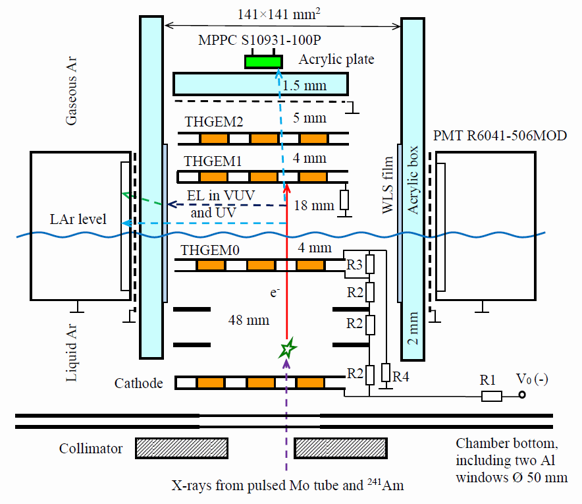
\includegraphics[width=0.8\textwidth]{install_scheme}}
\caption{����� ����������� ��������� ���������.}
\label{image:install_scheme}
\end{figure}

\section{����������� �������������� ������ ���� ������ �� ���� �������}
���� �� ������� ������� ����������� �������������� ������ ���� ������ ����������� � ��������� ���� ������������� ������� �������.
������ ����� ����� ��������� �����������. ���� �� ����������� ������� ���, ��� ���������� ����� ���� ��������� ������������� ����� ������ ��� ������������ ������� ���� ������.
��� ������������� ���� ������ ���������� � �������� 2.45 ��� ������������ ���������� ������������ ������� ���� ������ ���������� 233 ���.

������������� ����� ����������� ��� ��������� ����� ����������, ���������� ������������ � �������������� ������:
\begin{eqnarray}\label{eq:ionization_yield_defenition}
Q_{y} = n_{e} / E_{0}
\end{eqnarray}

���� ����������, ���������� ������������, ����������� ��������� ������� ����������� �� ����:
\begin{eqnarray}\label{eq:ne_Ni_field}
n_{e} / N_{i} = 1 / (1 + k(E) / \varepsilon)
\end{eqnarray}

� ����� ������ ����������� �� ������� ������� ��� ������ ����� ��� ���������:
\begin{eqnarray}\label{eq:ne_Ni_energy}
n_{e} / N_{i} = a(\varepsilon) / (1 + b(\varepsilon) / E)
\end{eqnarray}

������ � �������� $n_{e} / N_{i}$ ��� ����� 59.5 ��� ���, ������� �� ������� ��� �������� �������������.
������� ��� ��������� ������� ���������� �������� $n_{e} / N_{i}$, ��������� ����������� �������� ���� � ��������� (\ref{eq:ne_Ni_field}).
����� ������� ������ $n_{e} / N_{i}$ �� ������� � �������������� ��� ���������� (\ref{eq:ne_Ni_energy}), ����� ��������� $a$ � $b$.
��������� � ��������� (\ref{eq:ne_Ni_energy}) ������� 59.5 ���, �������� $n_{e} / N_{i}$ ��� ��������� ${}^{241}Am$.
����� �������� ������� ���������� �������� ������������ ��� ������� 59.5 ���:
\begin{eqnarray}\label{eq:ne_using_W}
n_{e} = \frac{n_{e}}{N_{i}} \cdot \frac{E}{W}
\end{eqnarray}
����� $W = 23.6$ ��� - �������, ����������� �� ������������ ����� �������� - ������ ����.
�� �����������, $W = E / N_{i}$.
��������� ��� ����������� � �������� ����� ��*� � ����� ���������� $n_{e}$ �� ��������� �������:
\begin{eqnarray}\label{eq:calibration_nVs_to_ne}
n_{e} = \frac{S[nVs]}{S^{Am}[nVs]} \cdot n_{e}^{Am}
\end{eqnarray}

���������� ������ ������ ������� � ����� ���������� $n_{e}$, ������ ���������� ������� ��� ��������� ��������������.
��-������, ���������� �� �������, ����������� ��� ������ ����������� ����������, ������� ������� �������, ���������� ��� ������-���� �������� ���������.
� �������� ����������� �������� ��������� ����������� ��� ����������� ��������� ������� ����.
��� ������� �������� ������� ������������ ����� �������� �� ����������� ������.
���� ������������� ����������� ���������� ������������ ������, �� ���� ��� ������� ���������� ������� ����� ������� �������� � �������� � ���������� ����.
����� ������� ��������� ��� ���� ����������� �� ������������� ������ ���� ������� - ������������� �������� �� ��������� � ������ �����-�������� ������ ���� �� ����� ������ ��� ���� ������������� �� ����������� ������. �������� �����-�������� ���� ���� � ������.

����� ��������� ���� ������, ���������� ��� ������ ����������� ����������, ��� ��� �������� ����� ������ ������.
��� ������ ���������� ��������� ���������� �����-������.
�� ������� ����� ������ �� ��������� ������������ ������������� ������� ���� �����.
������ �� ����� ��������, ���������� ��������� ������ ����� ���������� ����������� � ����������.
����� � ���������� ������������� ������� ���������� ���������� �����-������ � �������� 1294 ���.
������������ ��������� �������������� �����-������ ��� � �������, ��� � � ������� ����������� ����������� ����� ������������� ���������.
� ������� ������� ������� ���� ������ ������������� ������ ������ �� ����� � �������� �������.
��� ����� �������, ���� ���������������� ������ ��� ������� �������, ��� ���� �������.
��, ��� ���� ������� ����, ����� ����� ������ ����������� ������������� ��� ����������� ��������� ��� ��� ����������� ���������� ��������.
����� ��������� �����-�������� ���� ������� ��������� ������������� �������� �������� ����� �������.
����� �������, ����������� �������� $n_{e}$, ������� � ��������� ��������� (\ref{eq:ionization_yield_defenition}).

� ����������� ��������� (\ref{eq:ionization_yield_defenition}) ����� ���������� ������������ ������� ���� ������.
������������� ������ ����� ������ ������ ����, ��������������� ������������ ���������� �������.
������ �������� ����� �������� �������������� ����������, ������� ������ ���� �����������.
��� �������� ����� ������� ������������� �������������� ���������� ����������:
\begin{eqnarray}\label{eq:ER_resolution}
ER(E) = \frac{ER^{Am}}{E^{Am}} \cdot E
\end{eqnarray}
��� ����� ������� ����������� ����������� ��������������� ���������� �� ������� ���������� ������������ ������� � ������� ���������, ������ �� ������ ������ ���� ������� �� ��� ����������.
������������� ����� ������� �������� ��������, �� ������ ��������� ���� ������� � �������������� ��������.

���� �������� ����� ���������� $n_{e}$, ���������� �� ������������ �� ���� �������, �� ��������� ���� ������� � �������������� ��������, ��������� �� �������������, �� �� ������� ������������� ����� ��� ������� 233 ���. � ������� 2016 ���� ���� �������� �������� 5.9 � 7.4 e-/��� ��� 0.56 and 0.62 ��/�� ��������������.



\section{������� ��������� ���������}
�� ������ ������ ��������� �������� ��������� ���������� ��-�� ����, ��� ���������� ������ 25 ������� ������� SiPM, ��� ������������ ��� ����������� ���������� ���� ���������� ��������.
������ ����� ������ 25 ������� ������� ��� �����, � ��������� ������������� ������� ������.
� ��������� ����� ����� ������������ ��������� ��� ������������� ����������� ������ �� ���� ��������.

��� ������ ����������� ����������� ���������������� ���������� ��������� ���� ������������� � ��������� GEANT4.
��� �������� ���������� ������ ��������� ��������� ������������ ���������� ���������� ����� 2 ��.
����� ������������� ���������� ��� ������������� ��������������� ������, ����������� ��� ������������� ������ ������ �������.

\section{S1/S2 �������� ���������� ��������� � �����-�������}
�� ������ ������ ������ ������������ (DarkSide, ��������) ���������� ��� ���������� �����-���� S1 ������� � S1 ��������� ����������.
���� ����������� � ���, ��� �������� � �����-������ ����� ������ ��������� ���������.
��� ����� � ��� �� ������� ������� ��������� ��������� ����� ���� ��� ��������.
��� �������� � ����, ��� � ��������� ������ ����� ������� ����� ��������-������ ���, ������ ��� ���������, � ������ ����� ��������� ��� ������������.
������ ����� ������ �������� ��� ������� ��������� ����� (� ������������ DarkSide-50 ���� 200 �/��) � �� ����� ����� ��������.
��� ������ �������� (���� 5 ���) ������� � ��������� ��������� ���������� � ��������� ���������� �����, �, ����� ����, ����� ������� ���������� ���� ��� ����������� �������.
��� ��������� ������������� ������������� ������������� �������� ������� � ������� �������� ����������.
� ������������� �� ������ ������� ����� ���������� ���������� �� ���� ������� �������� S1 � S2 �������� ��� ��������� � �����-�������.
� ����� ������������ �� ����� �������� ����������� �������� ����������, ������ � ������ ������.
����� � ������ ������ ����� �������� ���������� �� �������������.

�� ������ ������ �������� ������� offline � ���������� �� ���������� ��������� � �����-�������� �� Na � �� ����������� ��������� ������ ��������, ��� ��������� S1 ���������� �� ��� ��������� �� ������ ������-���� ��������������. ����� ����� ���������� ������������������ �������������� ������������ �� ������ ��� ���������� ��������� �� �����-�������, �� � ��� ����������� �������������� ���������� ����� �������������� ����. ��� ��������� ���������� S1 ���������� ���� ������� ������� SiPM �������� 12$\times$12 ��������� ��� ��������� �� ��� ���������� ������, � ����� ��������� �������� ��������� � THGEM. 
\section{THGEM ���������� ������������}
������������ ����� S1 ���������� �������� ��� ����������� ����� THGEM0 � �������������� ������������� 27\% (��� ���������� ������� �����). ��� ��������� ���������� THGEM0 ����� ������� �� ����������� THGEM � ������� ��������� ���������. �� ������ ������ ����������� THGEM � ������������� 48\% ��� 75\% � ��������� 0.5 ��� 1 �� (����� ������ ��������� ����, �� ��� ����� ������� ����).
THGEM � ������� ������������� ����� ������� ������������ ���������. ������������� ����� ��������� �� ����������� THGEM ����������� ��������� ��� ������ ������������. 

\section{������������ ������� SiPM 12$\times$12}
��� ���������� ������� ��������� �� ��� ���������� ������ ����� �������� ������� SiPM 12$\times$12. �������� ������ �� 144 ������� ���������� � ����� � ��������������� �������� �������� � ����������� ������������ ����� ����������. ��� ������� ������ �������� ���� ���������� ���������� � ���� ����� ������ 9 SiPM, �������� 3 SiPM ���������������, � ����� ������ �� 3 ���������������� SiPM ��������� �����������. ��� ��� ���������� �����������-���������������� ���������� (NsNp).

������������ ���� ���������� ��������� � ���������� ������� ��������� ������� � ���������� (�� ����������� ���������� �������) ������������� ����� SiPM.  
���� ��������� ����� ������ ��� ���������������� (Ns) � ������������ (Np) ����������� SiPM.
��� � ���������, ��� ���������������� ����������� $N_s$ SiPM ��������� � �����(������� �������) ����������� � ~$N_{serial}$ ���, � ������ ���������� ������� ������ ��-�� ������� ���������� ��������.
��� ������������ ����������� $N_p$ SiPM ��������� ������������� �����������, ������������ ������� �������������, �� ����� ����� �������� �������.

������������� ������ �����������-����������������� ���������� ����� ������ � �� ������ ������ �� ��������.
��� �������� ������� �����������-���������������� ���������� ���������������� ���� �������������� �� ������ SiPM �������� �� ���, ��� ����� ����������� � ��������.
��-�� ������������ ������� ������� ���� �������� ����������, ��� ��� ���������� 3s3p ����� ������ �������� � 3 ����.
��� ����� ����������� ����������� ���������� �� ������� ������ SiPM.


%After-pulsing and cross-talk comparison for KETEK PM1125NS-SB0, Hamamatsu S10362-11-100C and Hamamatsu S13360-3050CS.

\section{Abstract}
Silicon photomultipliers (SiPMs) have become extensive used recently.
They exceed photomultiplier tubes on quantum efficiency, size and resistance to the magnetic field.
However, due to the features of the structure they have a greater value of dark noise rate, as well as they have additional sources of noise: cross-talk and after-pulsing.
In addition, these parameters may have a temperature dependence.

In this article we present results of a evaluation dark noise rate, probabilities of cross-talk and after-pulses at different voltages and temperatures for two modern SiPM: Hamamatsu S13360-3050CS and KETEK PM1125NS-SB0 and Hamamatsu S10362-11-100C SiPM from the previous generation.
An offline signal processing was performed by a pulse approximation with reconstruction of amplitudes and start times to find these parameters.
As a result, we found that at achieved measurement accuracy the dark noise rate has a temperature and a voltage dependence, but cross-talk and after-pulses probabilities have only the latter.

The measured cross-talk probabilities for KETEK PM1125NS-SB0 and Hamamatsu S13360-3050CS at their optimal operating voltage is about 6\%,
it is two times smaller than that for Hamamatsu S10362-11-100C.
The fast component of after-pulses probability for KETEK PM1125NS-SB0 and Hamamatsu S13360-3050CS is about 12\%, which is also almost 2 times smaller than sum of fast and slow components of after-pulses probability for Hamamatsu S10362-11-100C.
The dark noise rate for Hamamatsu S13360-3050CS at $ 20 \; ^{\circ}C $ is only $ 30 \; kHz / mm ^ 2 $ in comparison with $ 80 \; kHz / mm ^ 2 $ for KETEK PM1125NS-SB0.

\section{Introduction}
For many years BINP has been developing the X-ray inspection systems \cite{SiPM based photon counting detector for scanning digital radiography}.
These installations can be used in various fields: inspection at airports, subways or at workplaces.
Multistrip ionization chamber filled with pure Xe at 15 bar have been used as X-ray detector until now.
However, this detector has a disadvantage - it works in charge integrating mode, so at low input flow of particles electronic noise seriously degrades quality of images.
Another drawback is the insufficiently high detection efficiency of high-energy photons.
In this regard, it was decided to choose a new detector based on a SiPM and a scintillator which may has higher detection efficiency and will operate in the direct photon counting mode.

The main purpose of this work was to measure after-pulses and cross-talk probabilities for two SiPMs: KETEK PM1125NS-SB0 and Hamamatsu S13360-3050CS and compare them with the characteristics of Hamamatsu S10362-11-100C - the device from the previous generation.
\section{Measurement of breakdown voltage}
One of the important characteristics of any SiPM is a breakdown voltage.

In many works it was shown that SiPM gain is a linear function of both a temperature and a voltage.
Thus, the expression for gain $ G (V, T) $ is written as follows: \cite{Silicon Photomultiplier's Gain Stabilization, Temperature and Bias Voltage Dependence, Characterization of SiPM: temperature dependencies, Characterisation of a silicon photomultiplier device}:
\begin{eqnarray}\label{eq:G(V, T)}
G(V, T) = a \cdot V + b \cdot T + c
\end{eqnarray}

It is easy to find a breakdown voltage equating the gain from Eq.(\ref{eq:G(V, T)}) to zero :
\begin{eqnarray}\label{eq:V_bd(T)}
V_{BD}(T) = \frac{-(b \cdot T + c)}{a} = \frac{dV}{dT} \cdot T + const
\end{eqnarray}

In measurements an voltage error $\Delta V$ was estimated at 0.01 V, and a temperature error $\Delta T$ was estimated as the minimum temperature step 1 K divided by $\sqrt{12}$.

\section{�ross-talk and after-pulses probabilities finding algorithm}
\subsection{Background}
There are several algorithms for finding cross-talk probabilities.
One of them is to measure a dark noise rate at different thresholds \cite{Characterisation Studies of Silicon Photomultipliers}.
A cross-talk probability can be defined as the ratio of the rates with 1.5 photoelectrons(phe) and 0.5 photoelectrons threshold:
\begin{eqnarray}\label{eq:X_talk}
P_{X-talk} = \nu_{1.5 phe} / \nu_{0.5 phe}
\end{eqnarray}
However, this method has the significant disadvantage: after-pulses are indistinguishable from cross-talk if the former above a threshold.
Furthermore, this algorithm does not use information about a signal shape. It makes a dependence on the threshold more blurred and
makes a finding of the $ \nu_{1.5 pe}$ value more complicated.

An advanced algorithm should use an information about a waveform.
There are two approaches for a signal processing: deconvolution \cite{Modeling crosstalk in silicon photomultipliers} and an approximation with known waveform \cite{Characterization and Simulation of the Response, After-pulsingandcross-talkinmulti-pixelphotoncounters, Using MPPCs for T2K Fine Grain Detector}.
In our work we decided to use the method of signal approximation.

In the process of approximation we obtain amplitudes and time stamps of event.
Using this information we recover the time constants and probabilities for after-pulses.

After-pulsing is retriggering of a cell originating from a capture of electrons into traps during an avalanche and their subsequent release in a time interval from a few nanoseconds to several microseconds \cite{Characterisation Studies of Silicon Photomultipliers}.
After initial triggering a voltage in a cell decreases to a breakdown voltage and then will recover to its original value exponentially.

There are several processes, which may cause of a cell retriggering.
The first is after-pulsing.
Because of different physical reasons, there are two types of after-pulses:
fast and slow \cite{After-pulsingandcross-talkinmulti-pixelphotoncounters, Using MPPCs for T2K Fine Grain Detector, Characterization and Simulation of the Response}.
The second is a cell retriggering could be induced by thermal generated electrons.
Each of the processes have exponential distribution in time with its time constant $\tau$:
\begin{eqnarray}\label{eq:f(dt)_afterpulsing}
f(\Delta t) = \frac{1}{\tau} \cdot \exp(-\Delta t / \tau),
\end{eqnarray}
Measuring distribution distances between the pulses it is possible to characterize the time constants and the probabilities of processes leading to the triggering.

If we consider only one exponential process, probability $P(t)$ that in the interval from $0$ to $t$ the pulse does not exist and
in the interval from $t$ to $t + \delta t$ one pulse occurs is given by $P_{exp}(t) =  \nu \cdot e^{- t \cdot \nu} \cdot \delta t$, where $\nu$ - frequency of events for given process.
For more complicated case when dark pulses or one type of after-pulses are taken into account the required probability $P(t)$ can be written as follows:
\begin{eqnarray}\label{eq:probability_dt_simple}
P(t) = P\{ \text{there are not after-pulses from $0$ to $t + \delta t$} \} \cdot \\ \nonumber
P\{ \text{there is dark pulse from $t$ to $t + \delta t$} \} +  \\ \nonumber
P\{ \text{there is after-pulse from $t$ to $t + \delta t$} \} \cdot  \\ \nonumber
P\{\text{there are not dark pulses from $0$ to $t + \delta t$} \}
\end{eqnarray}

The contribution of each process is as follows:
\begin{eqnarray}\label{eq:probability_dt_simple_parts}
P\{ \text{there are not after-pulses from $0$ to $t + \delta t$} \} = (1 - p) + p \cdot e^{- \nu \cdot t} \\ \nonumber
P\{ \text{there is dark pulse from $t$ to $t + \delta t$} \} = (\nu_{dc} \cdot e^{- \nu_{dc} \cdot t}) \cdot \delta t \\ \nonumber
P\{ \text{there is after-pulse from $t$ to $t + \delta t$} \} = p \cdot ( \nu \cdot e^{- \nu \cdot t} ) \cdot \delta t  \\ \nonumber
P\{\text{there are not dark pulses from $0$ to $t + \delta t$} \} = e^{- \nu_{dc} \cdot t} \\ \nonumber
\end{eqnarray}

Thus, substituting probabilities in Eq.(\ref{eq:probability_dt_simple}) from Eq.(\ref{eq:probability_dt_simple_parts}) and reducing the resulting expression on $\delta t$ we obtain the probability density of pulse intervals:
\begin{eqnarray}\label{eq:probability_dt_fast}
f(t) = p \cdot (\nu + \nu_{dc}) \cdot e^{-(\nu + \nu_{dc}) \cdot t} + (1 - p) \cdot \nu_{dc} \cdot e^{-\nu_{dc} \cdot t},
\end{eqnarray}
where $p$ - probability of after-pulses.
It is worth noting that a similar formula is given in \cite{Using MPPCs for T2K Fine Grain Detector}, but with a typo in the sign between the terms.

As a result, taking into account the fast and slow components of after-pulses and dark noise events the probability density distribution of pulse intervals can be written as follows:
\begin{eqnarray}\label{eq:dt_probability_fast_slow}
f(t) = p_{s} \cdot p_{f} \cdot (\nu_{s} + \nu_{f} + \nu_{dc} ) \cdot e^{- (\nu_{s} + \nu_{f} + \nu_{dc}) \cdot t} + \\ \nonumber
p_{s} \cdot (1 - p_{f}) \cdot (\nu_{s} + \nu_{dc}) \cdot e^{- (\nu_{s} + \nu_{dc}) \cdot t} + \\ \nonumber
p_{f} \cdot (1 - p_{s}) \cdot (\nu_{f} + \nu_{dc}) \cdot e^{- (\nu_{f} + \nu_{dc}) \cdot t} + \\ \nonumber
(1 - p_{s}) \cdot (1 - p_{f}) \cdot \nu_{dc} \cdot e^{- \nu_{dc} \cdot t}
\end{eqnarray}

Eq.(\ref{eq:dt_probability_fast_slow}) is valid if one measure the distance between the signals caused by the triggering of a single cell.
Signals caused by the simultaneous triggering of two or more cells (because of cross-talk) shall be excluded from contribution.

In the article \cite{After-pulsingandcross-talkinmulti-pixelphotoncounters} it's shown another result for the probability density of pulse intervals which differ from presented here.
This is due to the consideration of one more process - delayed cross-talk.
However, in practice the probability of delayed cross-talk is much lower than the probability of direct cross-talk, and in our experiments we did not observe it.
The information about other processes that are responsible for a cell triggering can be found in \cite{Modeling crosstalk and afterpulsing in siliconphoto multipliers}.

\subsection{Signal finder}

Schematic overview of the experimental setup for recording SiPM signals is shown in Fig.\ref{image:install_V_bd_22}.

\begin{figure}[h]
\center{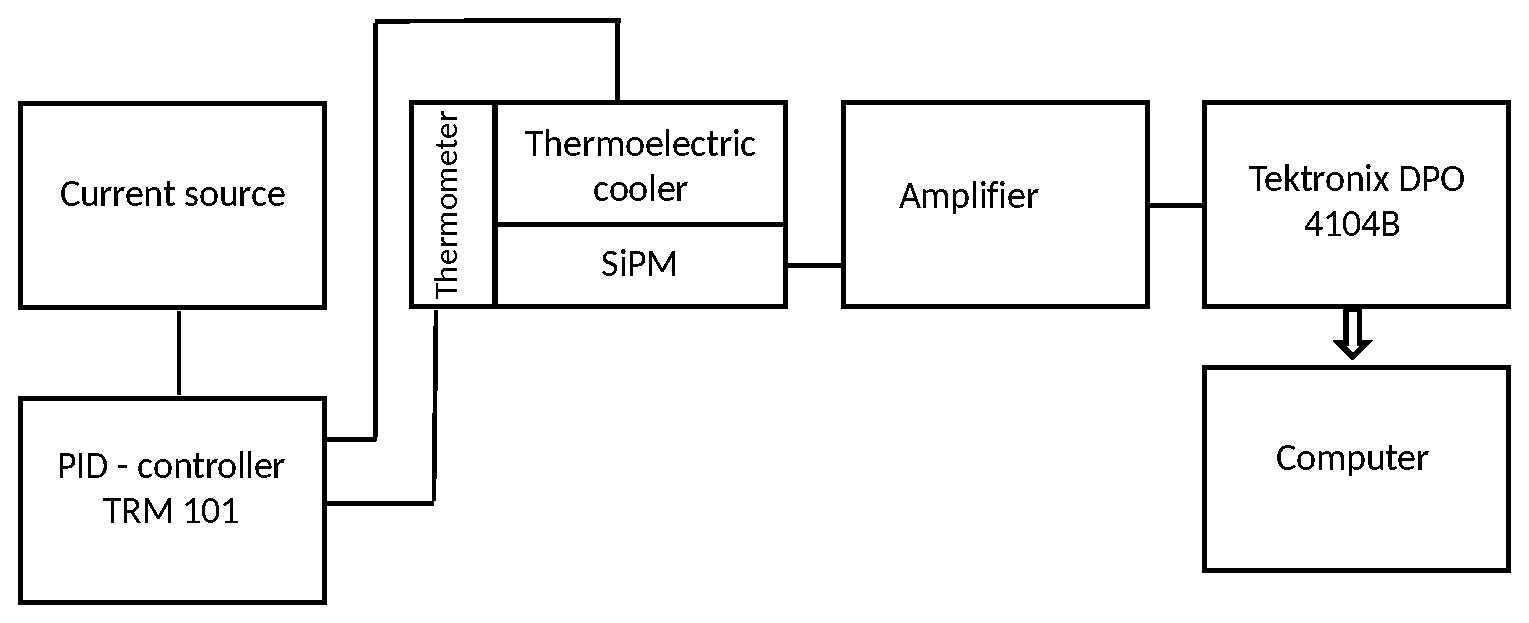
\includegraphics[width=8cm]{install_V_bd_22}}
\caption{Schematic overview of the experimental setup for recording SiPM signals.}
\label{image:install_V_bd_22}
\end{figure}

Raw data were recorded with Tektronix oscilloscope DPO 4104B with sample rate 5GHz and length 5M sample.
For each voltage and temperature combination 1000 files were recorded (total length is one second).

The signal can be presented as a sum of single-electron pulses $Signal_{1e}(t)$ with amplitude $A_{i}$ and start time $t_{i}$:
\begin{eqnarray}\label{eq:parsing}
V(t) = \sum \limits_{i = 0}^{N} A_{i} \cdot Signal_{1e}(t - t_{i}) + V_{0},
\end{eqnarray}
where $V_{0}$ is baseline level.

The waveform of the single-electron pulse was found from analysis of the recorded signal and was approximated by an analytical function.
The signal was processed by an algorithm that recover single-electron pulses without after-pulses impurities and averaged them.
The waveform samples of the single-electron pulses for different SiPMs are shown in Fig.\ref{image:signal_form_comparison}.
The waveforms were measured at different overvoltages and temperatures (from -8 to 27 $^{\circ}C$), but one remained practically unchanged.

\begin{figure}[h]
\center{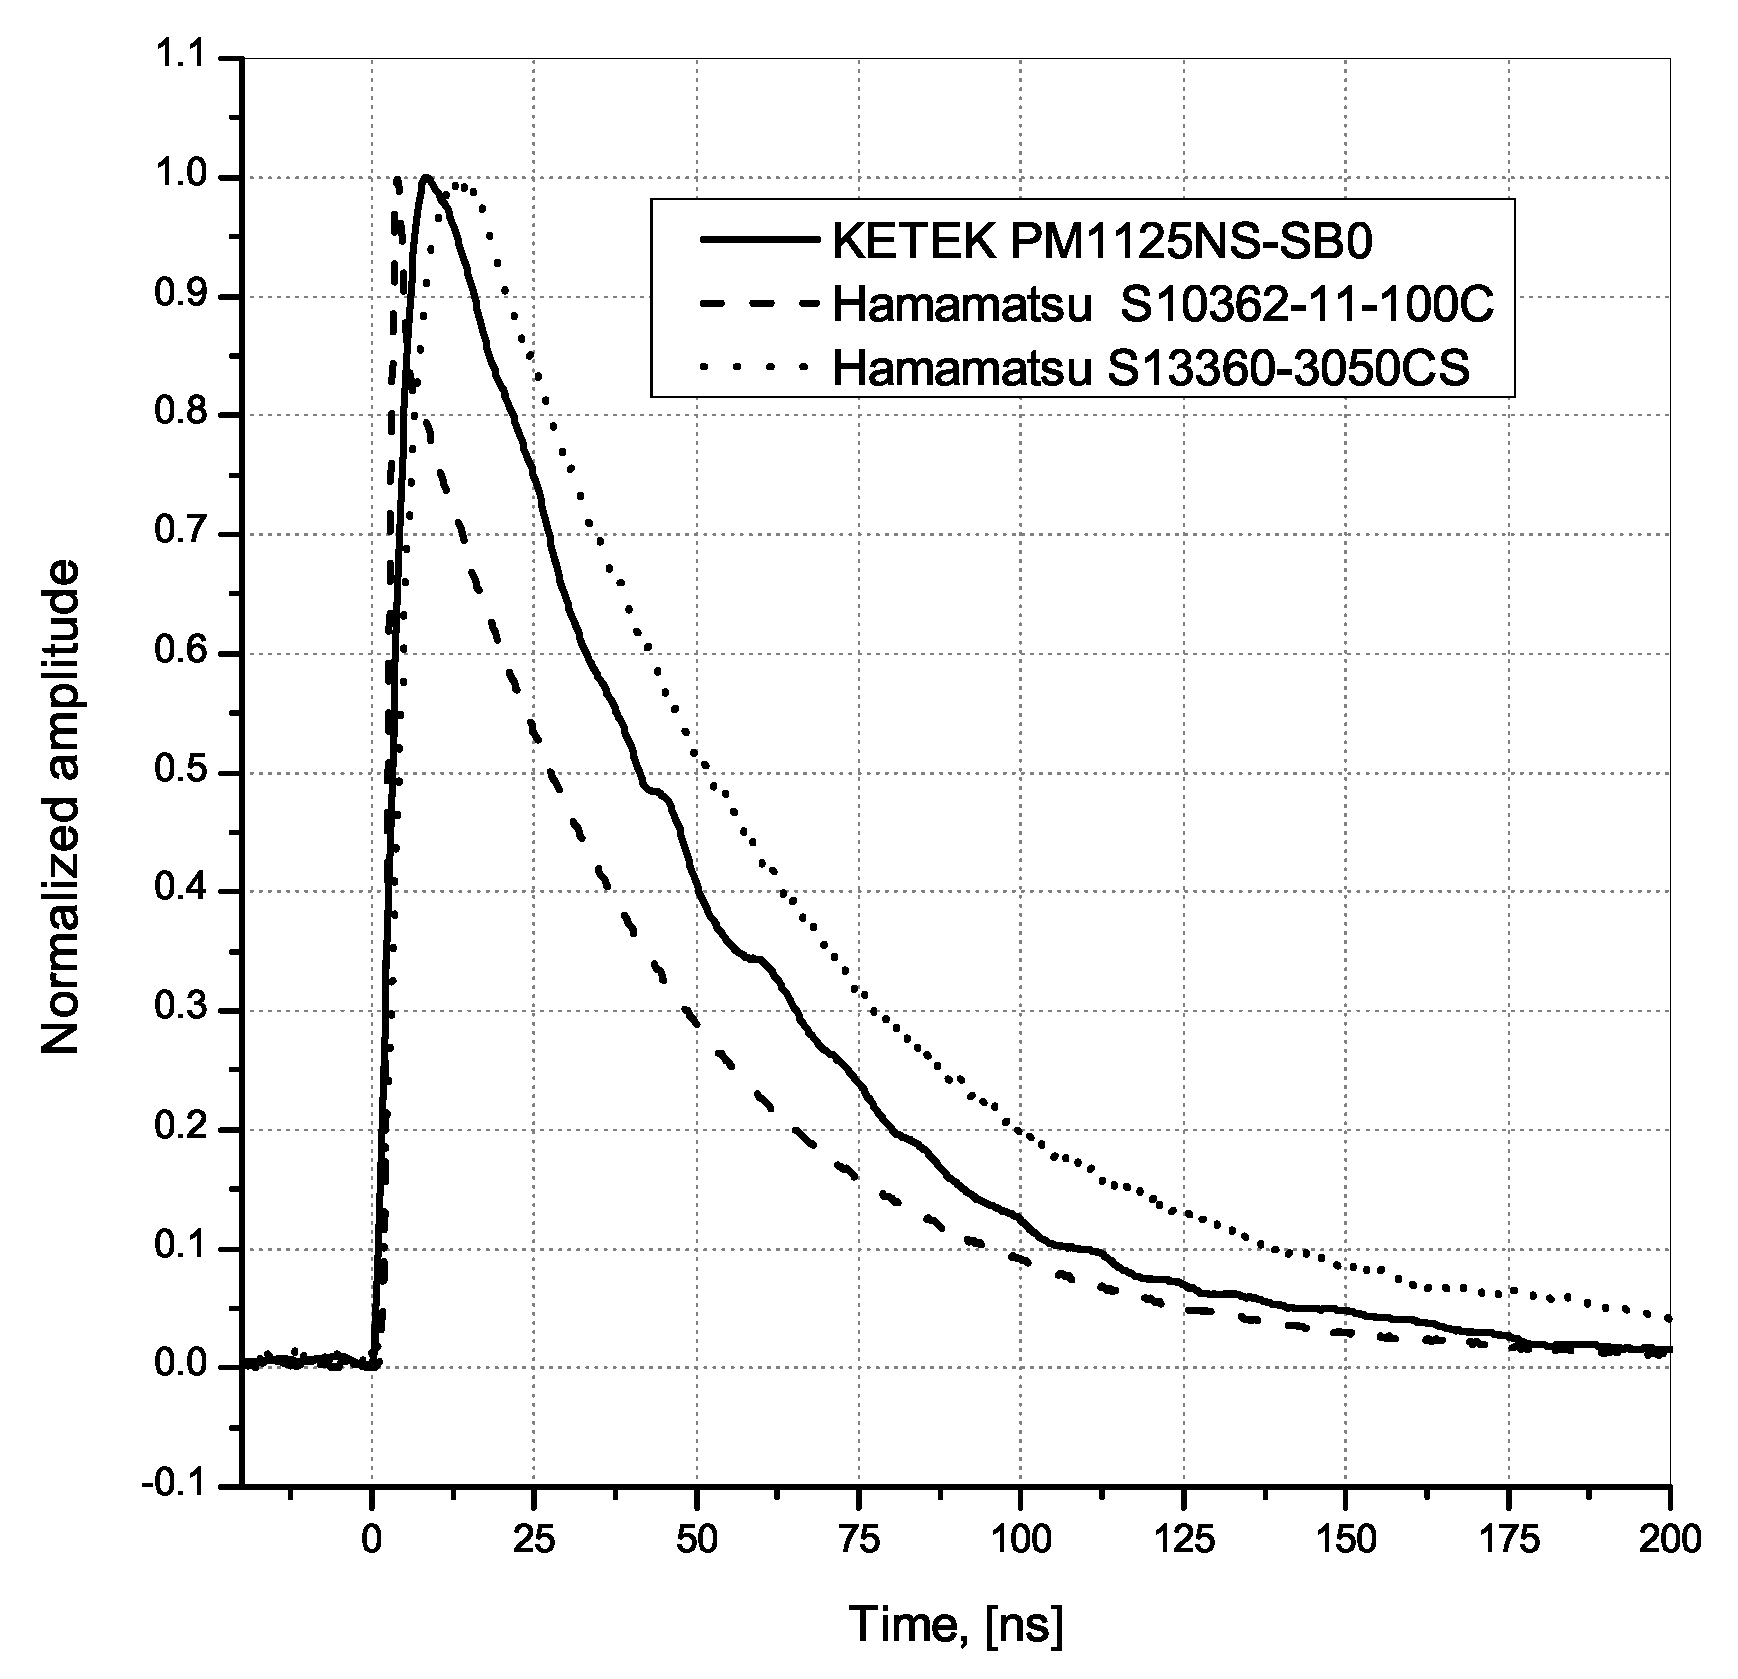
\includegraphics[width=8cm]{signal_form_comparison}}
\caption{The waveform of the single-electron pulse from different SiPMs.}
\label{image:signal_form_comparison}
\end{figure}

Further, single-electron pulses were approximated by a function obtained from the convolution of Eq.(\ref{eq:V(t)_base}) with the Gauss distribution describing a contribution of a limited operating speed of electronics.
The final expression is shown in Eq.(\ref{eq:V(t)_conv}).
\begin{eqnarray}\label{eq:V(t)_base}
V(t) = A \cdot \exp \left[- \frac{t - t_0}{\tau_{rec}} \right] \cdot \left( 1 - \exp \left[ -\frac{t - t_0}{\tau_{rise}} \right] \right) \cdot \theta(t - t_0) + V_0,
\end{eqnarray}

\begin{eqnarray}\label{eq:V(t)_conv}
V_{conv}(t) = V_0 + \frac{A}{2} \cdot \Bigg( \left\{ F(\sigma, \tau_{rec}) - F(\sigma, \tau_{total}) \right\} \Bigg), \text{ where} \\ \nonumber
F(\sigma, \tau) = \exp\left[ \frac{\sigma^2 - 2 t \cdot \tau}{2 \tau^2 } \right] \cdot \left( 1 + Erf \left[ \frac{t - \sigma^2 / \tau}{ \sigma \sqrt{2} } \right] \right), \\ \nonumber
\tau_{total} = \frac{\tau_{rec} \cdot \tau_{rise}}{\tau_{rec} + \tau_{rise}}
\end{eqnarray}
where $A$ - a pulse amplitude, $t_0$ - a time delay, $\tau_{rec}$ - a recovery time of a cell,
$\tau_{rise}$ - a rise time of a rising edge, $V_0$ - an offset, $\theta(t - t_0)$ - the Heaviside step function,
$\sigma$ - the standard deviation of the Gauss distribution.

The main task was to find $A_{i}$, $t_{i}$ parameters of individual pulses.
We can approximate a continuous waveform with 5MSamples length with Eq.(\ref{eq:parsing}) and $N \sim 30 \div 300$, but this task requires a huge amount of computing power. 
A continuous waveform were divided to practically independent fragments with $N = 1$ or $N = 2$ for the most parts.

The main problem with a processing a noise.
There are a lot of digital filters that can smooth a signal, but their use will lead to a loss of the information about after-pulses.
After-pulses are exponentially distributed in time and with a high probability they occur at short times, when a cell has not yet recovered.

An accuracy of signals location can be improved if we transmit into the peak finder algorithm initial parameters close to true ones.
For this purpose a signal derivative was calculated with the simultaneous smoothing (Savitsky-Golay third-order filter with the number of points equal to 51 (10.2 ns) )
Thus, the information about the derivative was also involved in the processing.

To split a recorded file into multiple independent fragments, we used the following algorithm: \\
1) The first derivative was calculated using the Savitsky-Golay filter. \\
2) If a derivative and an amplitude were higher of the threshold values $th_{der}$ and $th_{amp}^{start}$ then the time 20 ns before this event with $t_{trig}$ time was taken as start time $t_{start}$ of a signal.
This condition was necessary for the proper calculation of a baseline of the signal.\\
3) If after $t_{trig}$ time more than $\tau_{amp}^{dead} = 5 ns$ passed and the signal level was below the threshold amplitude $th_{amp}^{stop}$ and
ahead on 20 ns the derivative was below the threshold $th_{der}$, then this time was the end time of the signal.
The amplitude threshold $th_{amp}^{stop}$ was chosen as the intersection of the signal with the baseline.

To determine $th_{amp}^{start}$ a dependence of events number versus the threshold voltage at different values of the dead time $\tau_{amp}^{dead}$ was measured. 
The examples of dependencies are shown in Fig.~\ref{image:Hamamatsu_S10362-11-100C_295K_1OV_amp_th} for Hamamatsu S10362-11-100C at $T = 295K$ and $\Delta V = 1 V$.
The thresholds were practically independent of the selected dead time $\tau_{amp}^{dead}$.
The threshold for a triggering by amplitude $th_{amp}^{start}$ was chosen at 1/2 amplitude of the single-electron signal (approximately $20V$).


A similar graph can be drawn for the derivative (Fig.~\ref{image:Hamamatsu_S10362-11-100C_295K_1OV_der_th}).
We selected only those signals that exceed the amplitude threshold $th_{amp}^{stop} = 2mV$, because without this condition the distribution would be significantly distorted.
Above the threshold value $4 \cdot 10^{-4} V / s$  the contribution of noise is significantly suppressed.
This value was selected as $th_{der}$.
Thresholds $th_{der}$ and $th_{amp}^{start}$ should be recalculated for other overvoltages.

\begin{figure}[h]
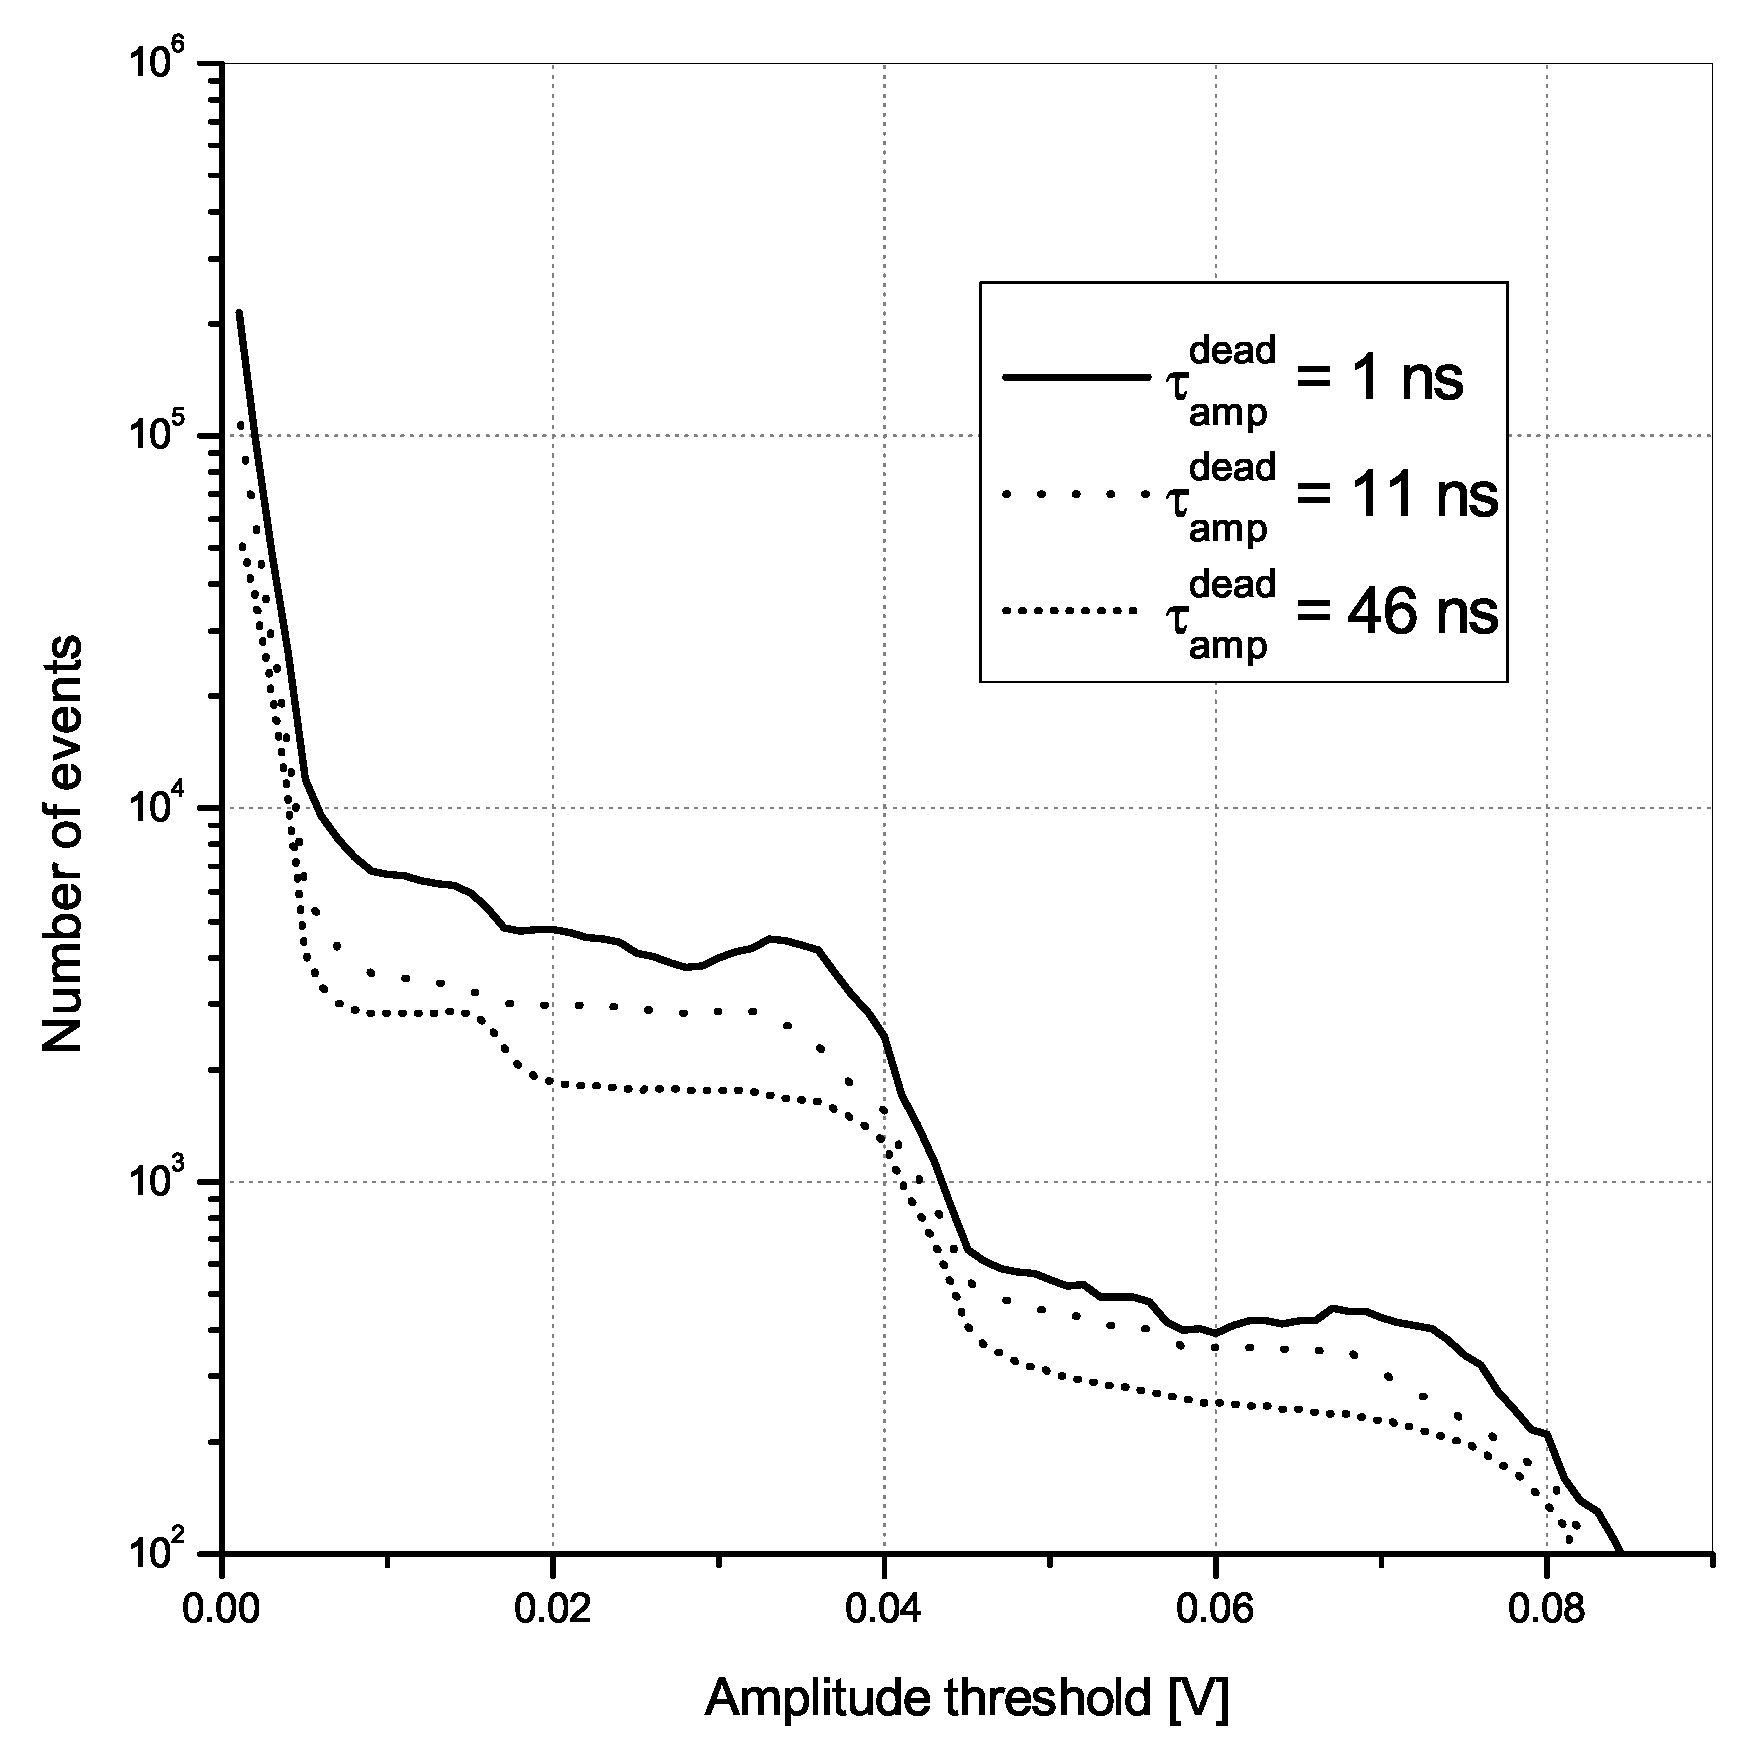
\includegraphics[width=0.47\textwidth]{Hamamatsu_S10362-11-100C_295K_1OV_amp_th_eng}
\hfill
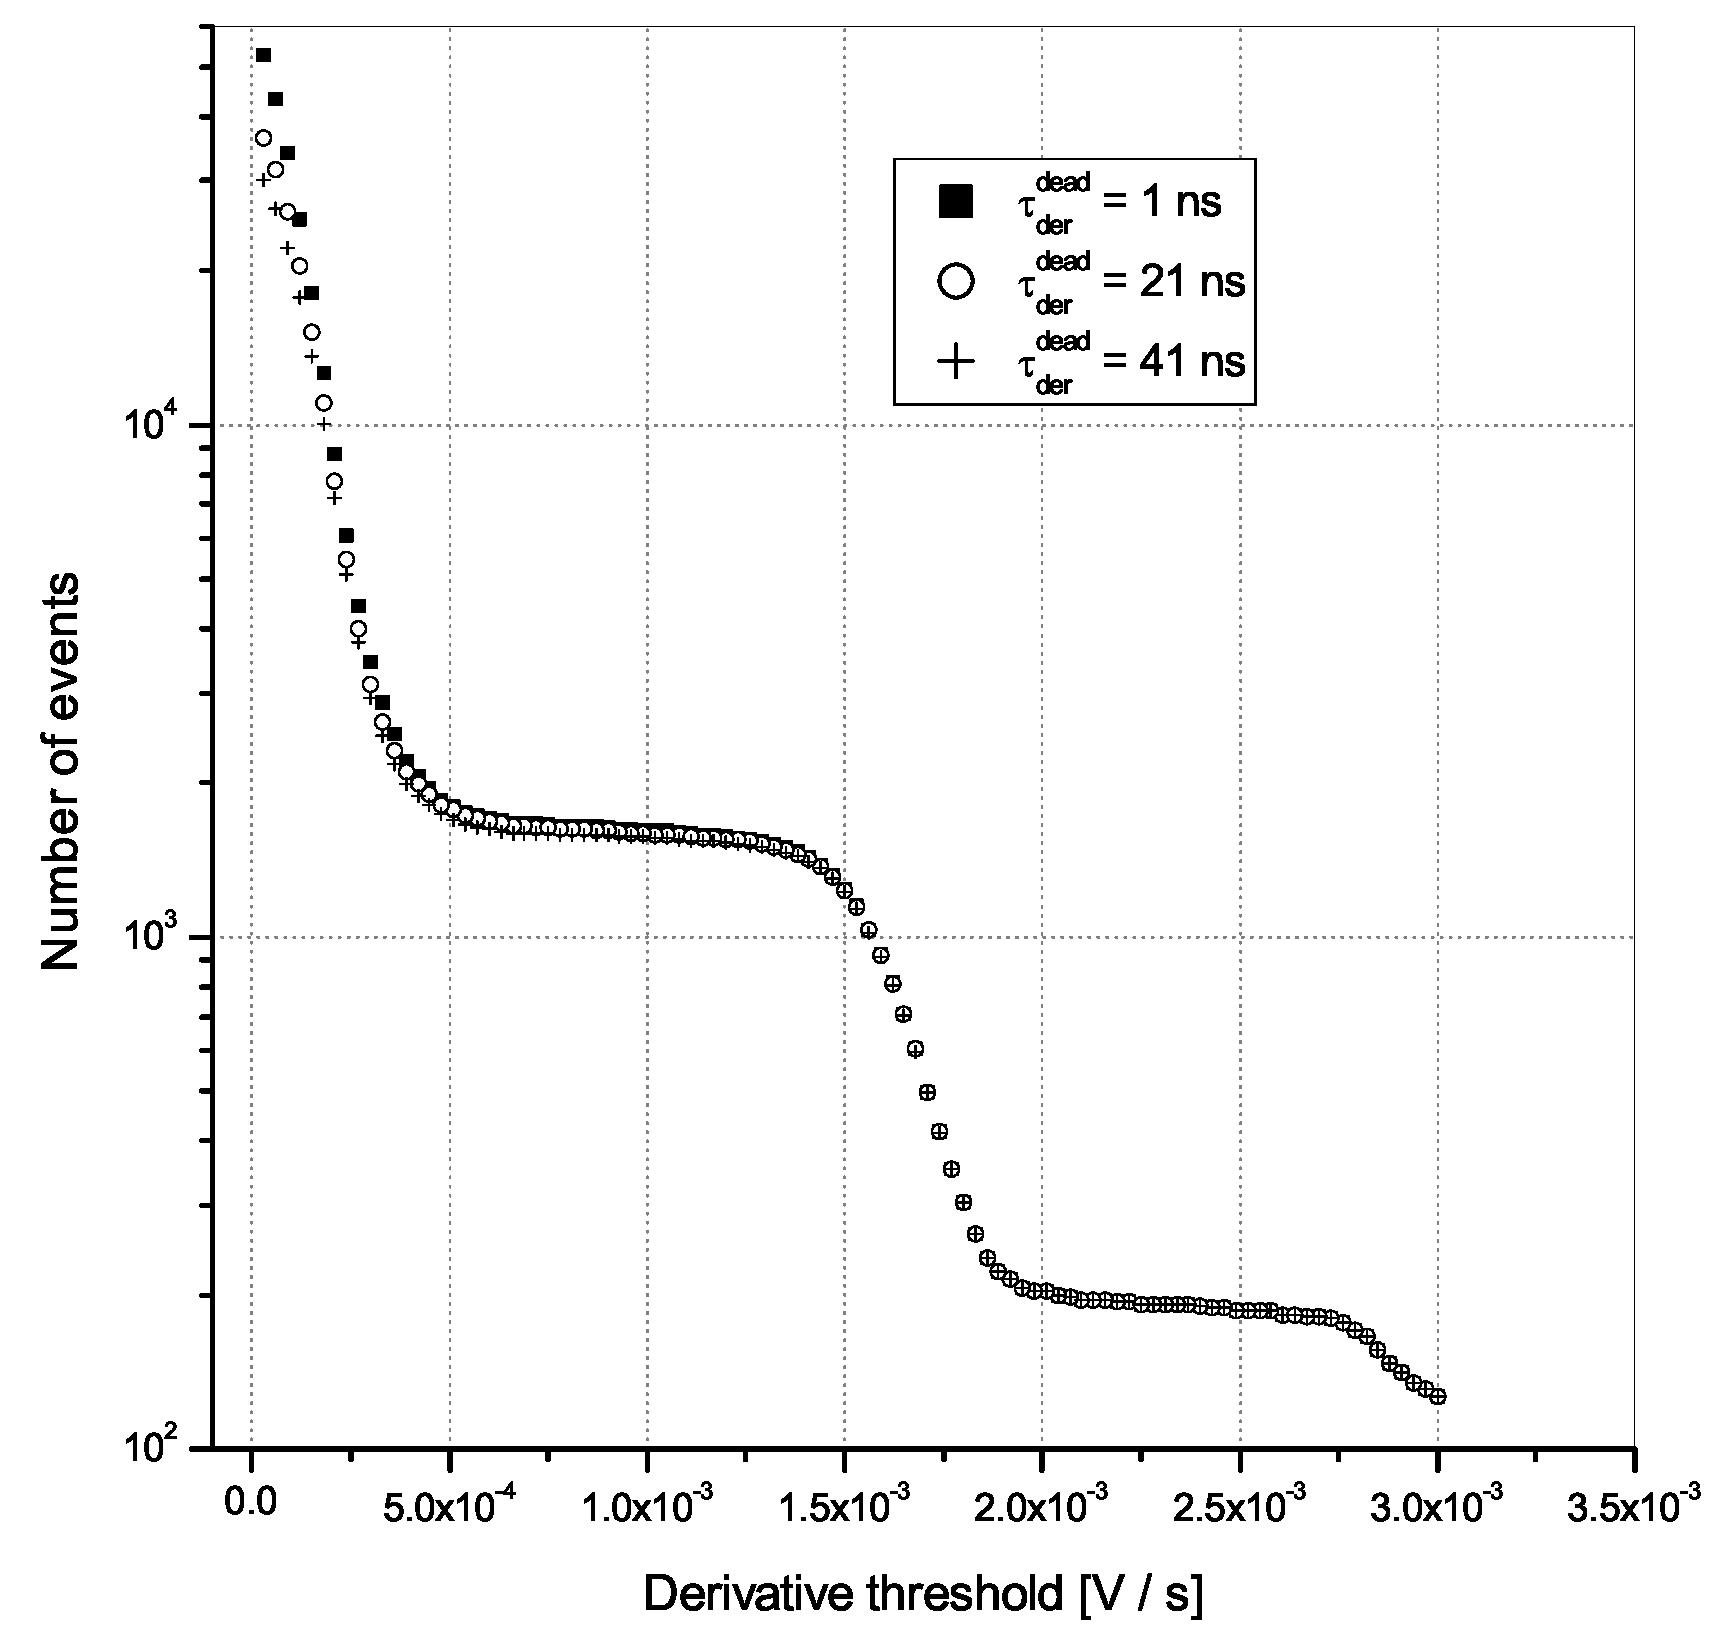
\includegraphics[width=0.47\textwidth]{Hamamatsu_S10362-11-100C_295K_1OV_der_th_eng}
\\
\parbox[t]{0.47\textwidth}{\caption{The dependence of the number of found signals from the amplitude threshold and the dead time $\tau_{amp}^{dead}$ for
Hamamatsu S10362-11-100C at 1V overvoltage and 295K temperature.}
\label{image:Hamamatsu_S10362-11-100C_295K_1OV_amp_th}}
\hfill
\parbox[t]{0.47\textwidth}{\caption{The dependence of the number of found signals from the derivative threshold and the dead time $\tau_{der}^{dead}$ for
Hamamatsu S10362-11-100C at 1V overvoltage and 295K temperature. Only signals exceeding the threshold $th_{amp}^{stop} = 0.002 V /s$ were selected.}
\label{image:Hamamatsu_S10362-11-100C_295K_1OV_der_th}}
\end{figure}

After this data processing the data files were divided into multiple independent fragments.
At each part had to either one pulse or superposition of pulses.
\subsection{Correlation analysis}

To find parameters $A_{i}$ and $t_{i}$ each part have to be approximated by Eq.(\ref{eq:parsing}).
This function internally nonlinear on the $t_{i}$ parameter therefore it is necessary to set the initial parameter of the start time of a signal.
To do this, we used the following algorithm:\\
1) If the first derivative was above the threshold, then we were looking for a derivative maximum from a current time to a current time plus 5 ns.
The time at which the first derivative reached the maximum used as the initial value of the $t_{i}$ parameter.\\
2) If the first derivative was below the threshold value and passed more than 5 ns then was allowed to search for the next threshold exceeding.\\

Further, an each independent part was approximated by Eq.(\ref{eq:parsing}) at $N = 1$.
Consider the correlation between the amplitude and $\chi^2 / Dof$ (Fig.~\ref{image:Hamamatsu_S10362-11-100C_295K_1V_Chi2_amp 1}).
One can notice a few outlying clusters: $A_{1}$, $B_{1}$, $C_{1}$ etc.
The cluster $A_{1}$ corresponds to single-electron signals.
Clusters $B_{1}$, $C_{1}$ etc. corresponds to events when simultaneously triggered two, three or more cells (cross-talk), and these signals was located away from other signals.
Because of this they have the low $\chi^2 / Dof$ value at the approximation of a single-component function.
Other events with the $\chi^2 / Dof > 4$ value (we denote them as $Z_{1}$ cluster ) correspond to several signals, located at a relatively short distance distance from other.

In the next step the events from the $Z_{1}$ cluster were approximated by Eq.(\ref{eq:parsing}) at $N = 2$.
In that case, each event is characterized by four parameters: $\chi^2 / Dof $, $amp_{1}$ and $amp_{2}$ - amplitudes of the first and the second signals, $\Delta t$ - a distance between the signals.
Draw a correlation between the total amplitude $amp_{1} + amp_{2}$ and a $\chi^2 / Dof $ value (Fig.~\ref{image:Hamamatsu_S10362-11-100C_295K_1_OV_Chi2_amp1_amp2}).

\begin{figure}[h]
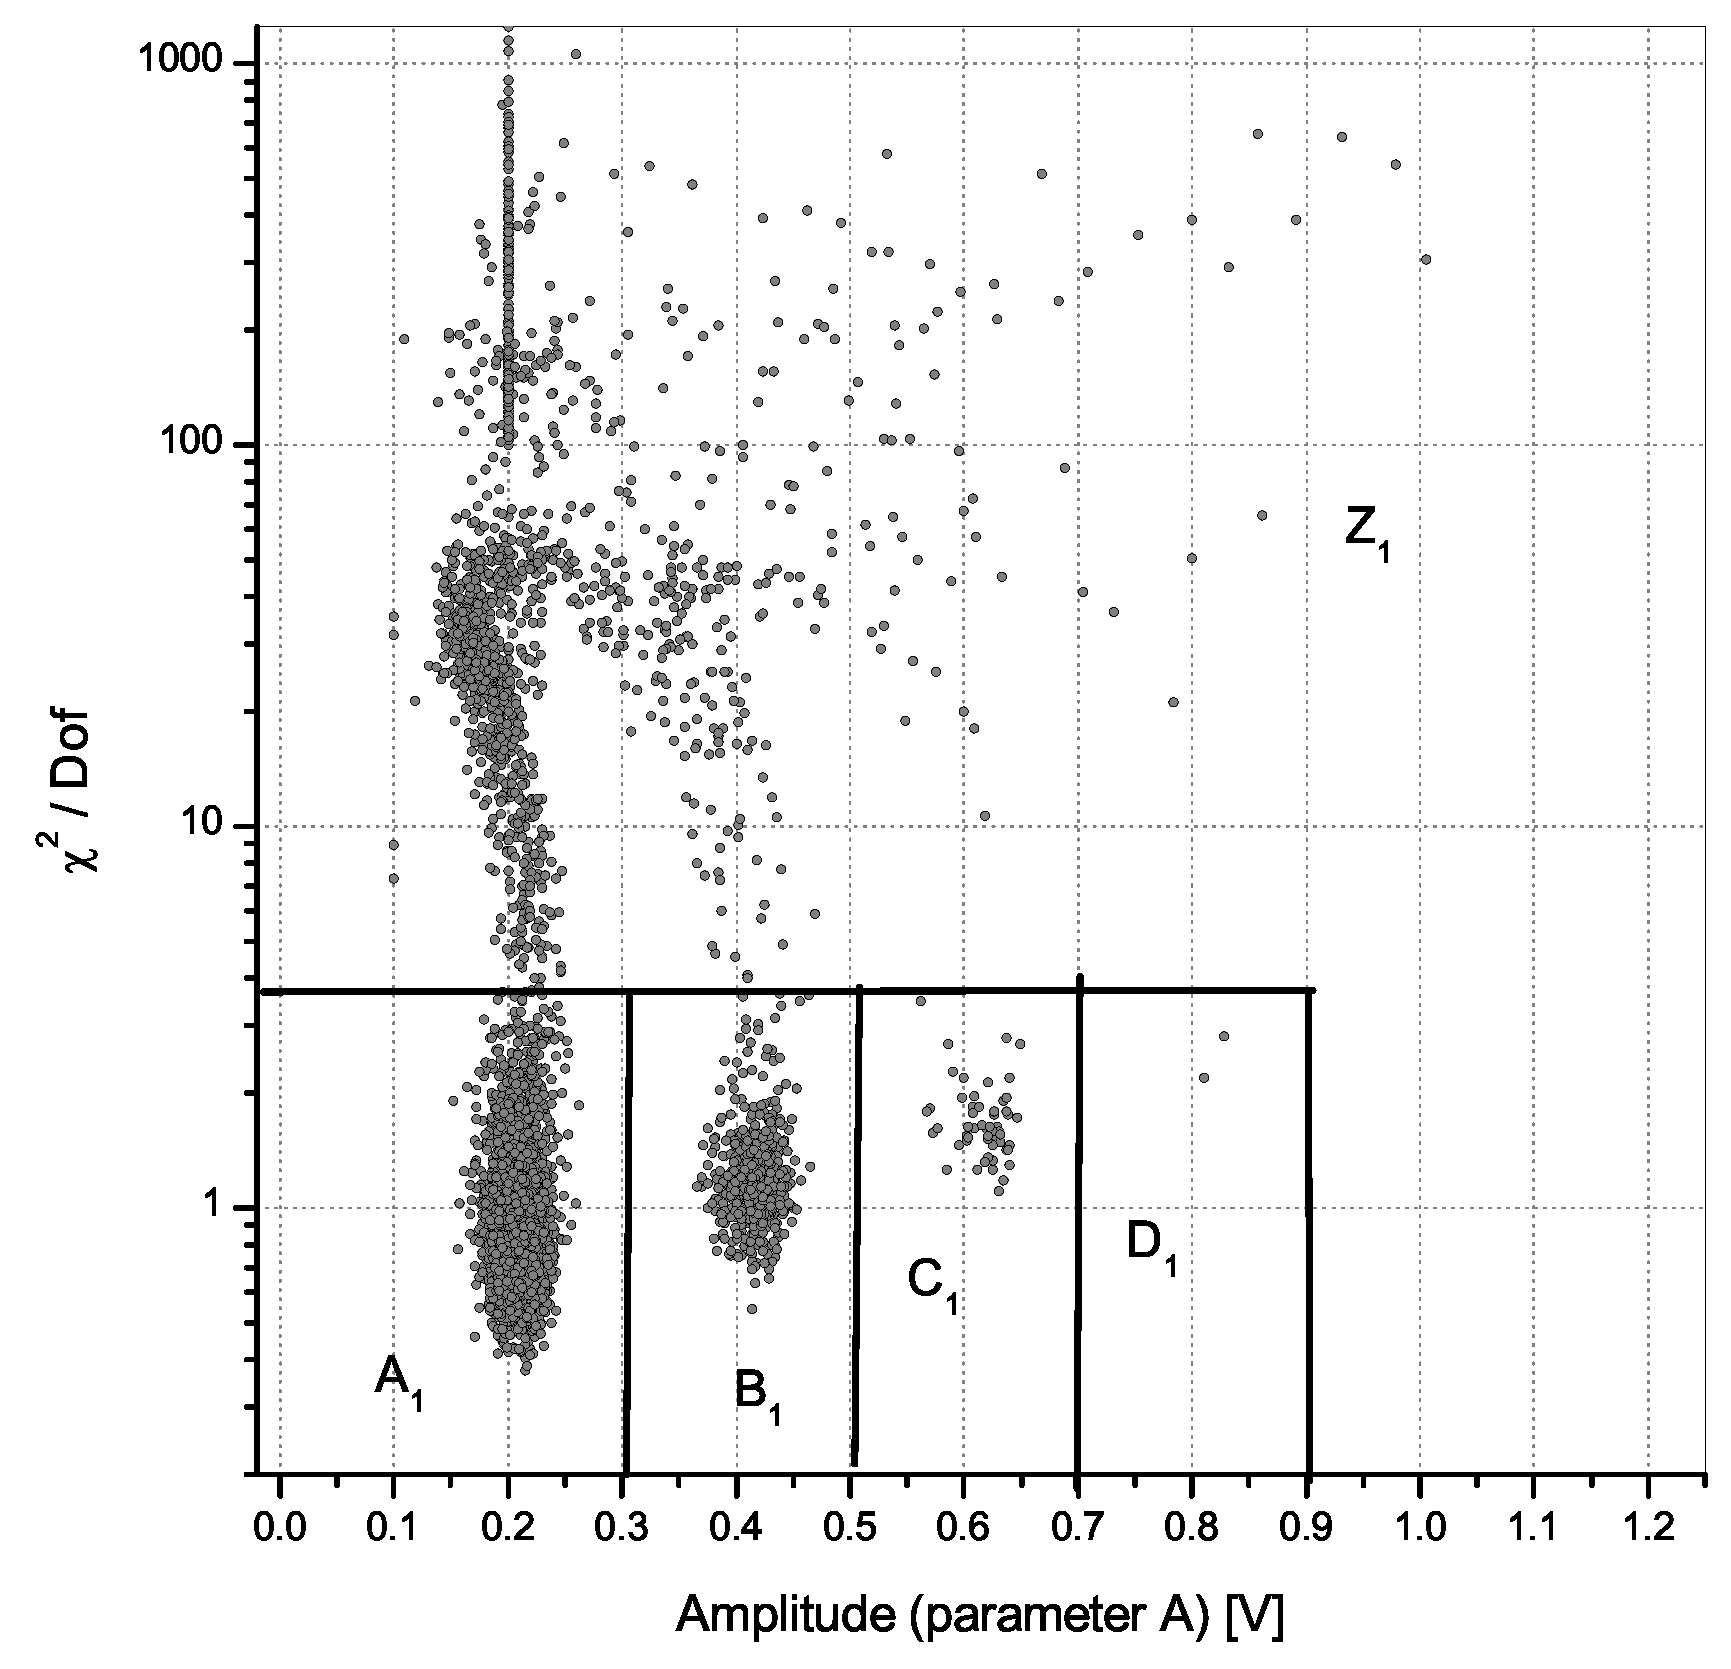
\includegraphics[width=0.47\textwidth]{Hamamatsu_S10362-11-100C_295K_1V_Chi2_amp_1}
\hfill
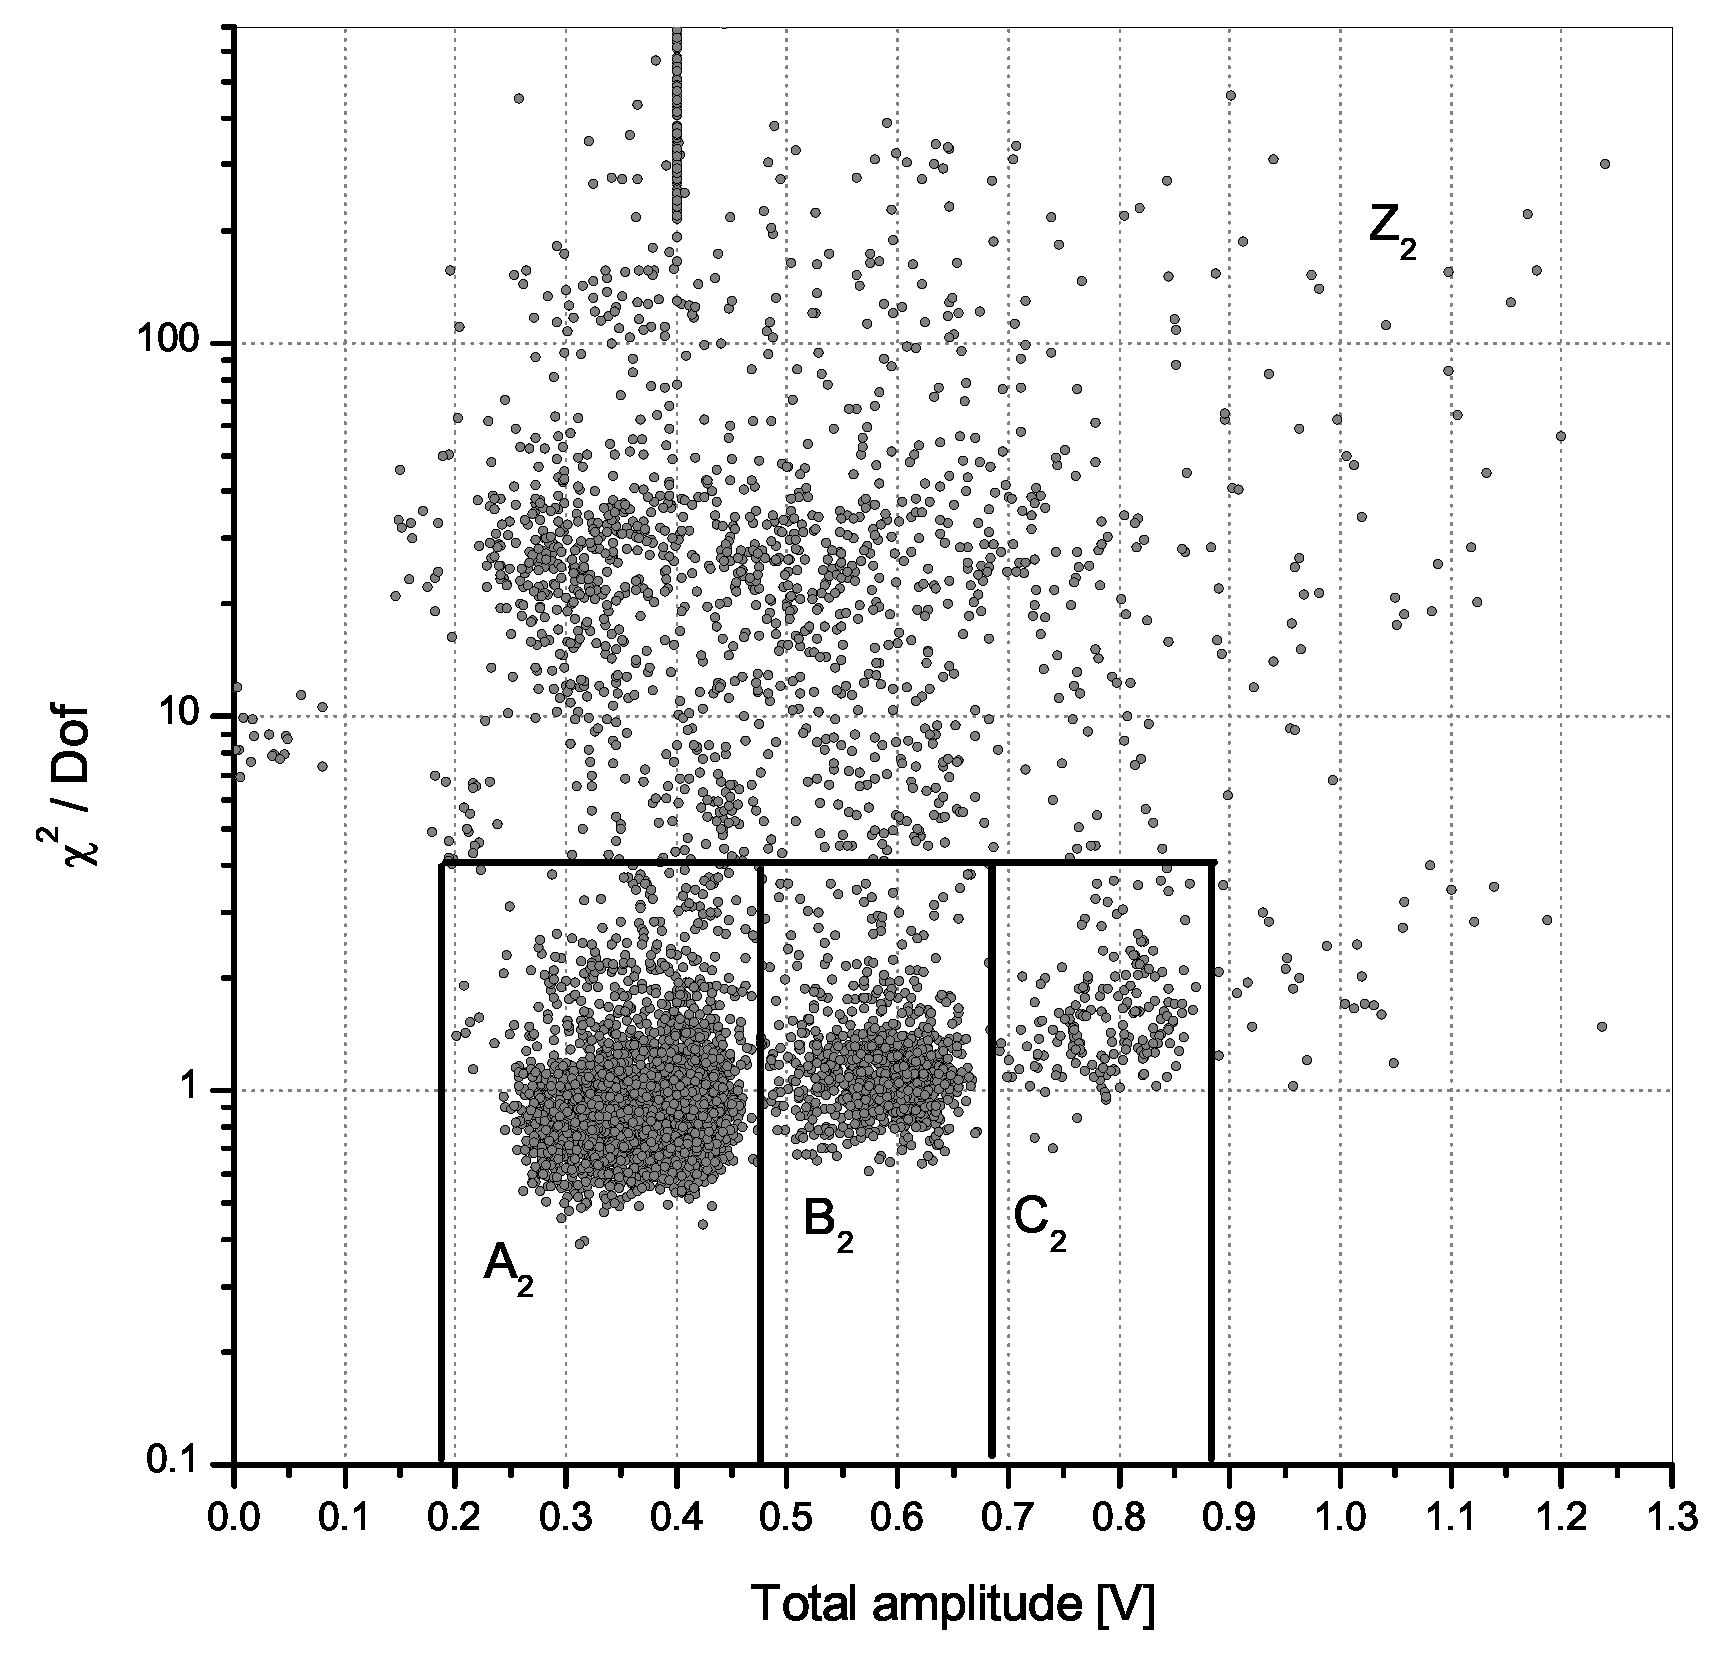
\includegraphics[width=0.47\textwidth]{Hamamatsu_S10362-11-100C_295K_1_OV_Chi2_amp1_amp2_eng}
\\
\parbox[t]{0.47\textwidth}{\caption{The correlation between the total amplitude $amp_{1} + amp_{2}$ and $\chi^2 / Dof$ when approximating all pulses by one-component function.
The signal was obtained from Hamamatsu S10362-11-100C at 1V overvoltage and 295K temperature.}
\label{image:Hamamatsu_S10362-11-100C_295K_1V_Chi2_amp 1}}
\hfill
\parbox[t]{0.47\textwidth}{\caption{The correlation between the total amplitude $amp_{1} + amp_{2}$ and $\chi^2 / Dof$ when approximating the $Z_{1}$ cluster (see Fig.~\ref{image:Hamamatsu_S10362-11-100C_295K_1V_Chi2_amp 1}) by two-component function.
The signal was obtained from Hamamatsu S10362-11-100C at 1V overvoltage and 295K temperature.}
\label{image:Hamamatsu_S10362-11-100C_295K_1_OV_Chi2_amp1_amp2}}
\end{figure}

In this case also there are several typical clusters: $A_{2}$, $B_{2}$, $C_{2}$ etc.
A more clear idea about the signals forming these clusters can be obtained from the correlation of $amp_{1} + amp_{2}$ and $\Delta t$ constructed for a particular cluster (Fig.~\ref{image:Hamamatsu_S10362-11-100C_295K_1_OV_amp1_amp2_dt_A2} and Fig.~\ref{image:Hamamatsu_S10362-11-100C_295K_1_OV_amp1_amp2_dt_B2}).

\begin{figure}[h]
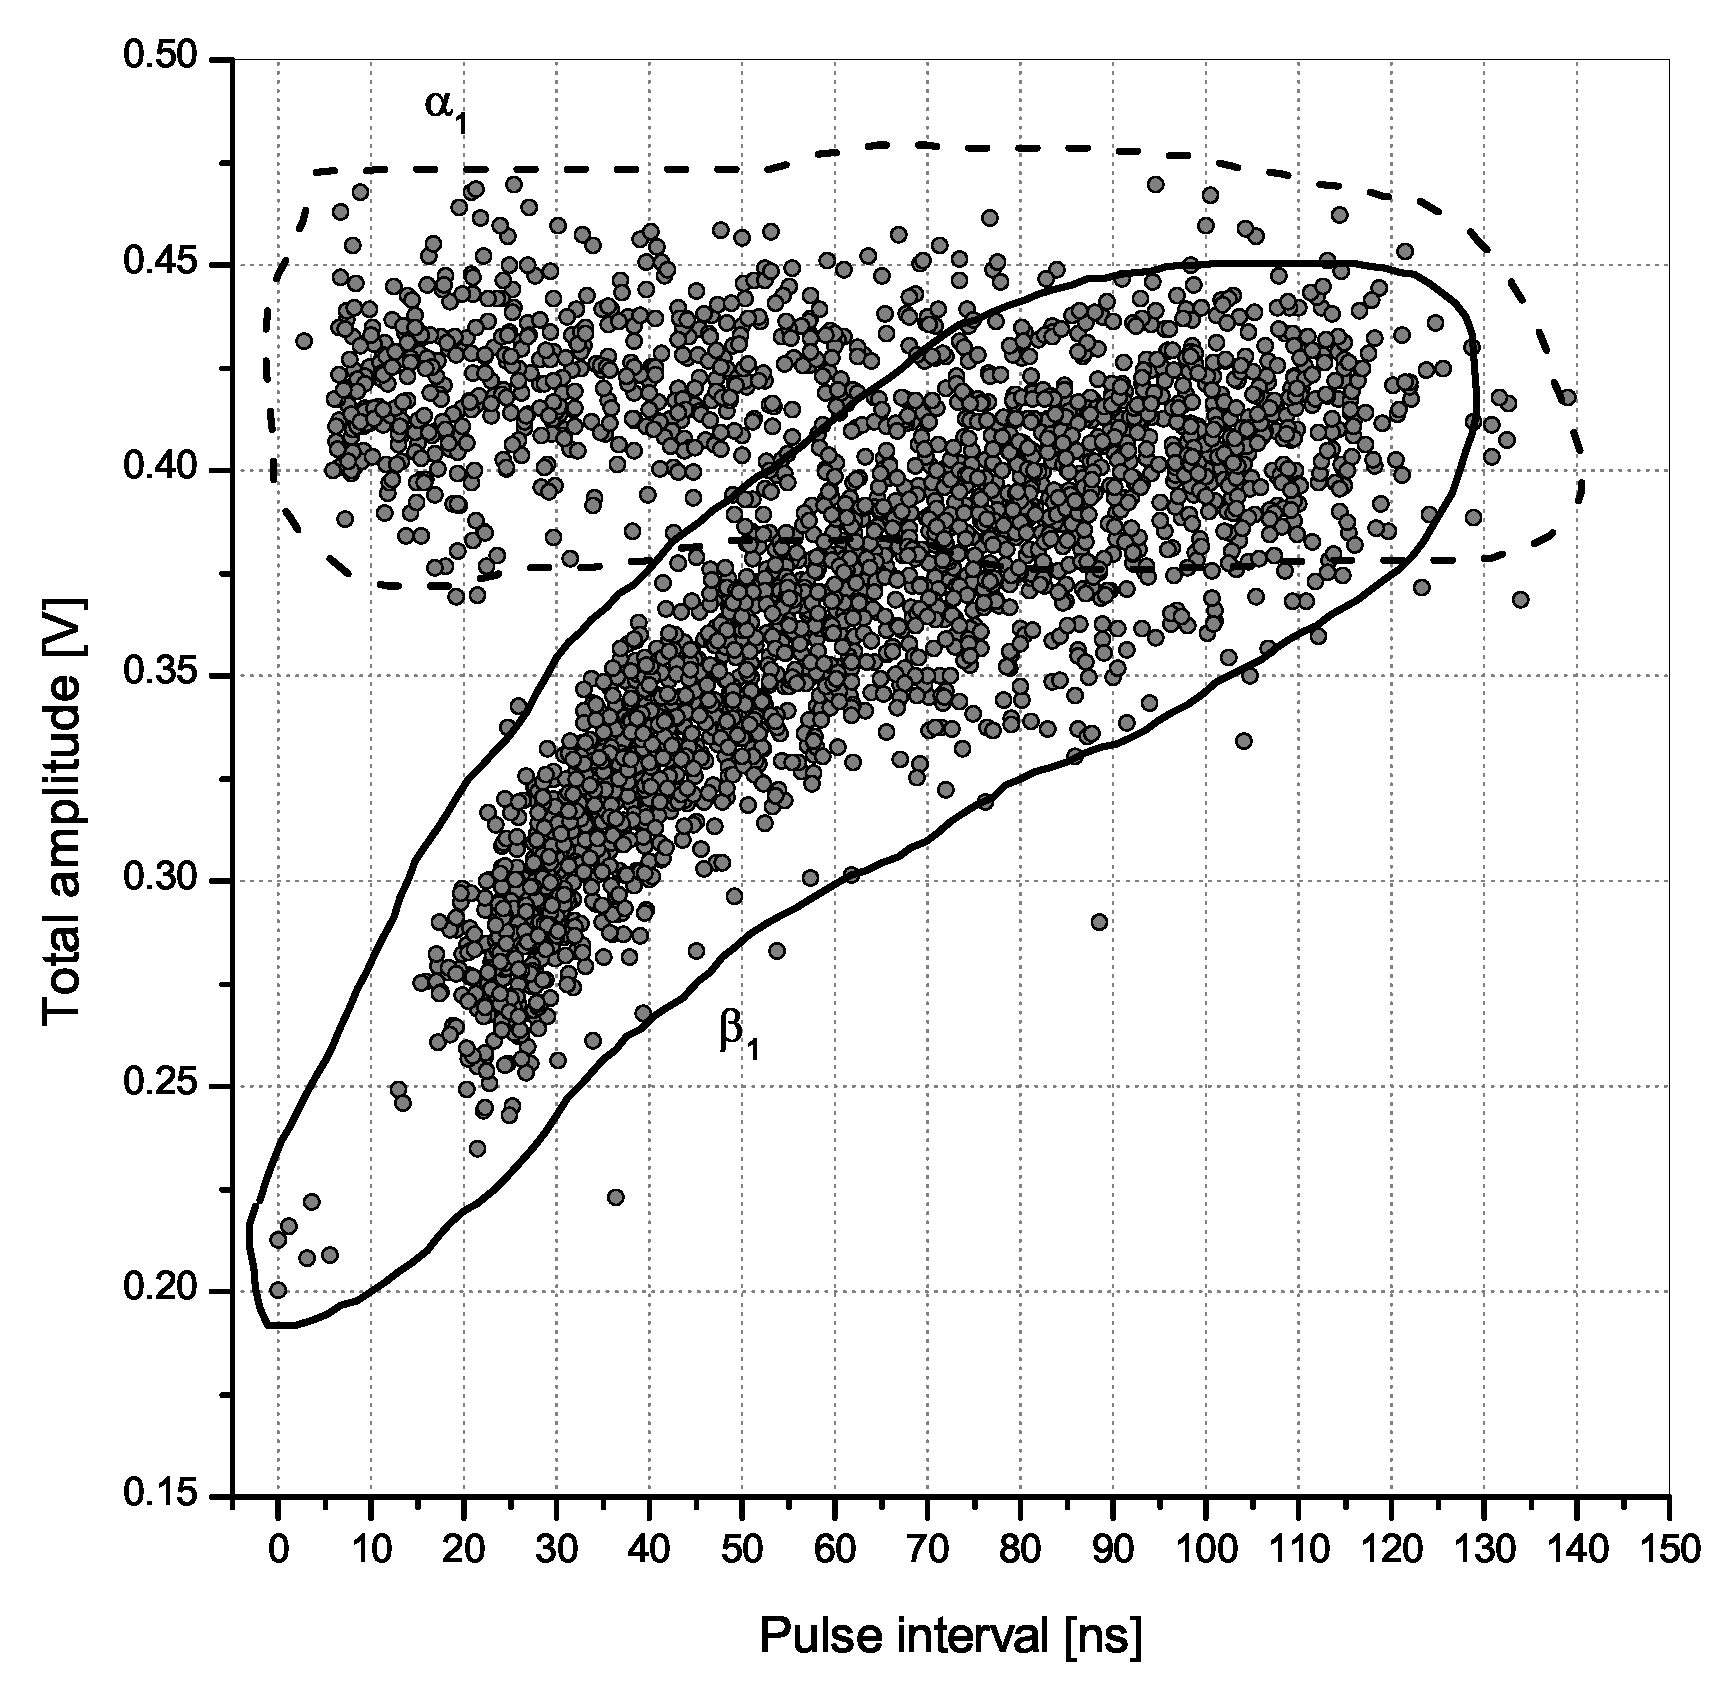
\includegraphics[width=0.47\textwidth]{Hamamatsu_S10362-11-100C_295K_1_OV_amp1_amp2_dt_A2_eng}
\hfill
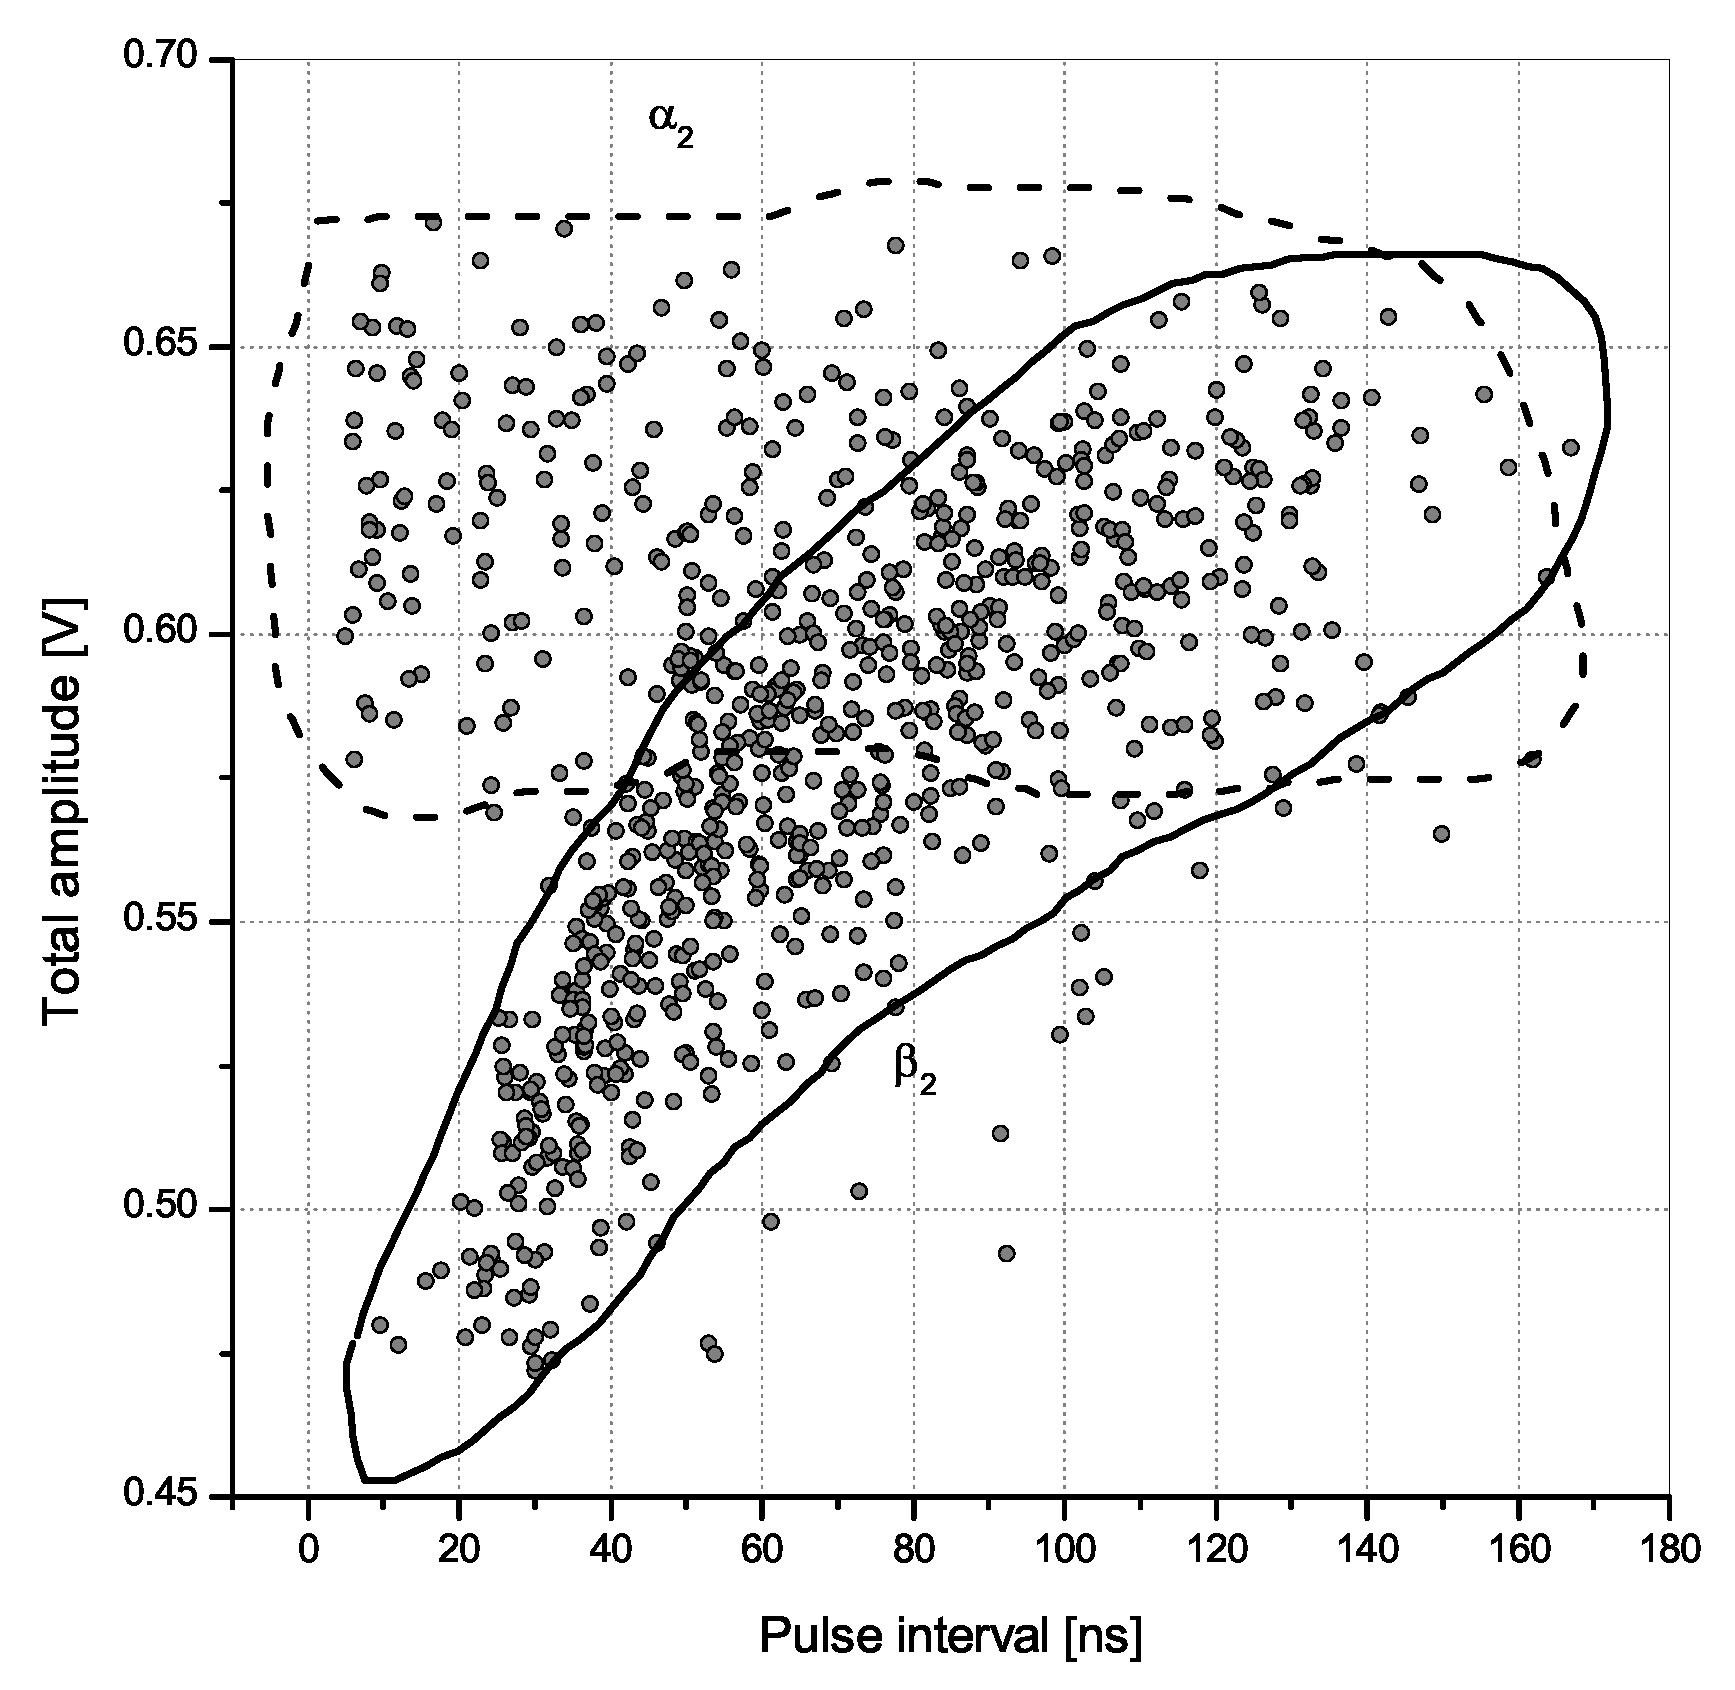
\includegraphics[width=0.47\textwidth]{Hamamatsu_S10362-11-100C_295K_1_OV_amp1_amp2_dt_B2_eng}
\\
\parbox[t]{0.47\textwidth}{\caption{The correlation between the pulse interval and the total amplitude when approximating the $A_{2}$ cluster
(see Fig.~\ref{image:Hamamatsu_S10362-11-100C_295K_1_OV_Chi2_amp1_amp2}) by two-component function.
The signal was obtained from Hamamatsu S10362-11-100C at 1V overvoltage and 295K temperature.}
\label{image:Hamamatsu_S10362-11-100C_295K_1_OV_amp1_amp2_dt_A2}}
\hfill
\parbox[t]{0.47\textwidth}{\caption{The correlation between the pulse interval and the total amplitude when approximating the $B_{2}$ cluster
(see Fig.~\ref{image:Hamamatsu_S10362-11-100C_295K_1_OV_Chi2_amp1_amp2}) by two-component function.
The signal was obtained from Hamamatsu S10362-11-100C at 1V overvoltage and 295K temperature.}
\label{image:Hamamatsu_S10362-11-100C_295K_1_OV_amp1_amp2_dt_B2}}
\end{figure}

The $A{2}$ cluster consists of signals that are conventionally divided into two sets: $\alpha_{1}$ �  $\beta_{1}$.
The set $\alpha_{1}$ corresponds to two closely spaced signals and their total amplitude equal to double amplitude of the single-electron pulse.
This means that these signals were caused by triggering of various cells and they are dark noise.
At the same time signals from the set $\beta_{1}$ have an amplitude that depends on the distance between signals.
This means that the first signal was a single-electron signal and the subsequent signal was an after-pulse.
The similar correlation can be constructed for the $B_{2}$ set (Fig.~\ref{image:Hamamatsu_S10362-11-100C_295K_1_OV_amp1_amp2_dt_B2}).
In this case, the set $\alpha_{2}$ consists of two closely spaced signals one of which has a single-electron amplitude.
Another signal has the double amplitude caused by the simultaneous triggering of two cells due to cross-talk.

The set $\beta_{2}$ contains signals that can be divided into two groups.
The first group was formed by signals in which two cells triggered simultaneously and then one of cells generated an after-pulse.
The second group was formed by signals in which one cell triggered and then after-pulse occurred which caused cross-talk.
The sets similar to $A_{2}$ and $A_{2}$ with a large total amplitude correspond to the events with a greater number of simultaneously triggered cells.

Then we built pulse interval spectrum.
We took into account only the signals without cross-talk, i.e. we measured the distance only between those signals that belong to the $A_{1}$ or $A_{2}$ clusters.
In the first approximation we can neglect events in the $A_{3}$, $A_{4}$ etc. clusters due to their small number relative to events in the $A_{1}$ or $A_{2}$ clusters.

As a result, we obtained the pulse interval spectrum shown in Fig.~\ref{image:Hamamatsu_S10362-11-100C_295K_1_OV_dt_spectrum}.
By approximating the spectrum by Eq.(\ref{eq:dt_probability_fast_slow}) we found $p_{s}$, $p_f$, $\nu_{s}$, $\nu_{f}$, $\nu_{DC}$ parameters.
For the approximation RooFit package and unbinned fit were used.

As you can see there is a change in the spectrum monotony when the pulse interval equals approximately 25 ns.
If the after-pulse occurs with the pulse interval less than 25 ns after the previous pulse, its amplitude is small and this pulse cannot be distinguished from noise.
Because of this the signal is recognized as a single component and it does not contribute to the short times.
This distorts the spectrum.
For the correct approximation we took into account only pulse intervals exceed a certain "threshold" value.
To clarify this value approximation was performed at different threshold values.
The dependence of the $\tau_{f}$ parameter from the pulse interval threshold is shown in Fig.~\ref{image:Hamamatsu_S10362-11-100C 295K_1_OV_dt_spectrum_timecut}.
For this type of SiMP at 295K temperature and 1V overvoltage 25 ns threshold was chosen.
When reducing the overvoltage the pulse interval threshold increases.

\begin{figure}[h]
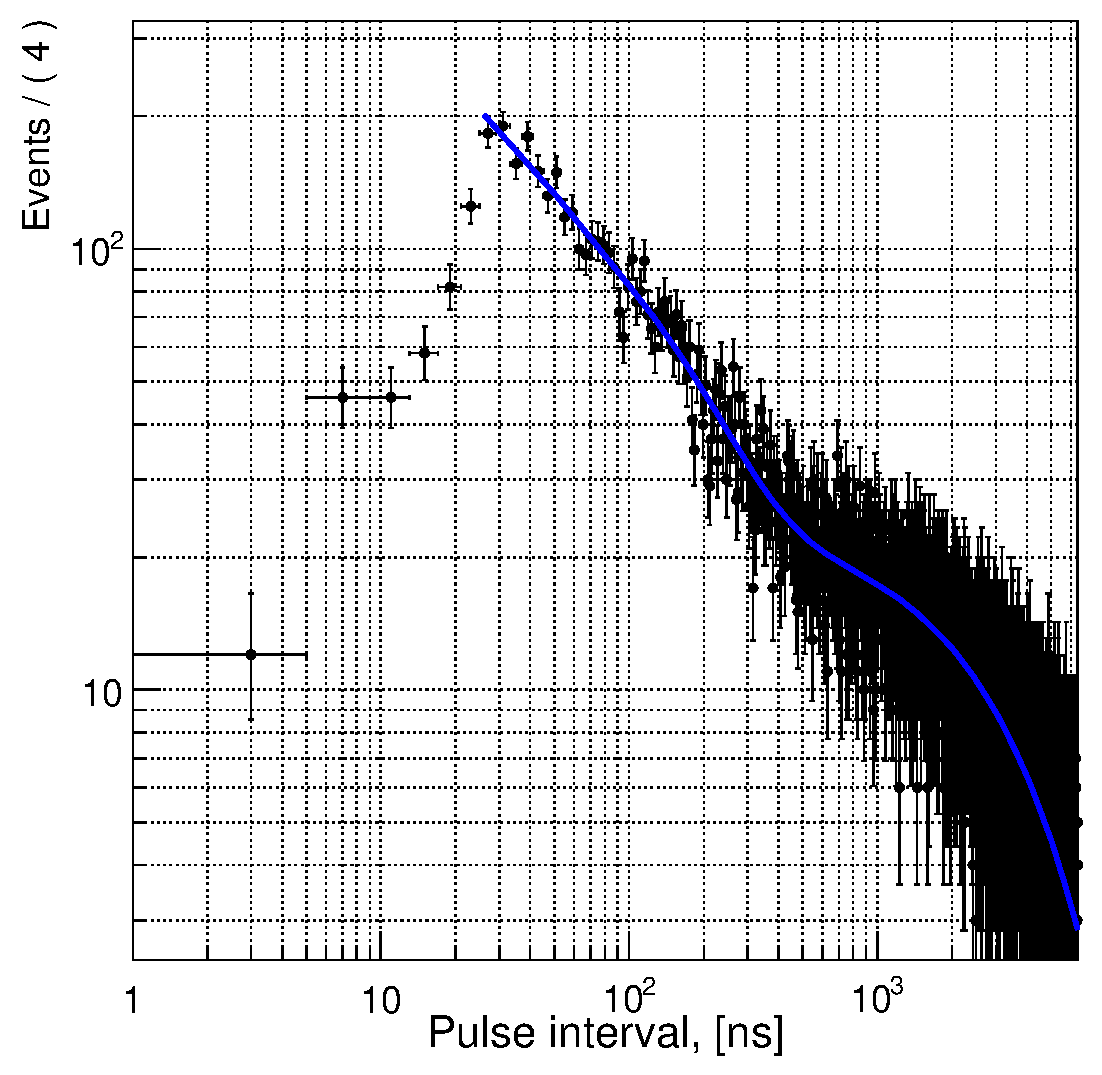
\includegraphics[width=0.47\textwidth]{Hamamatsu_S10362-11-100C_295K_1_OV_dt_spectrum}
\hfill
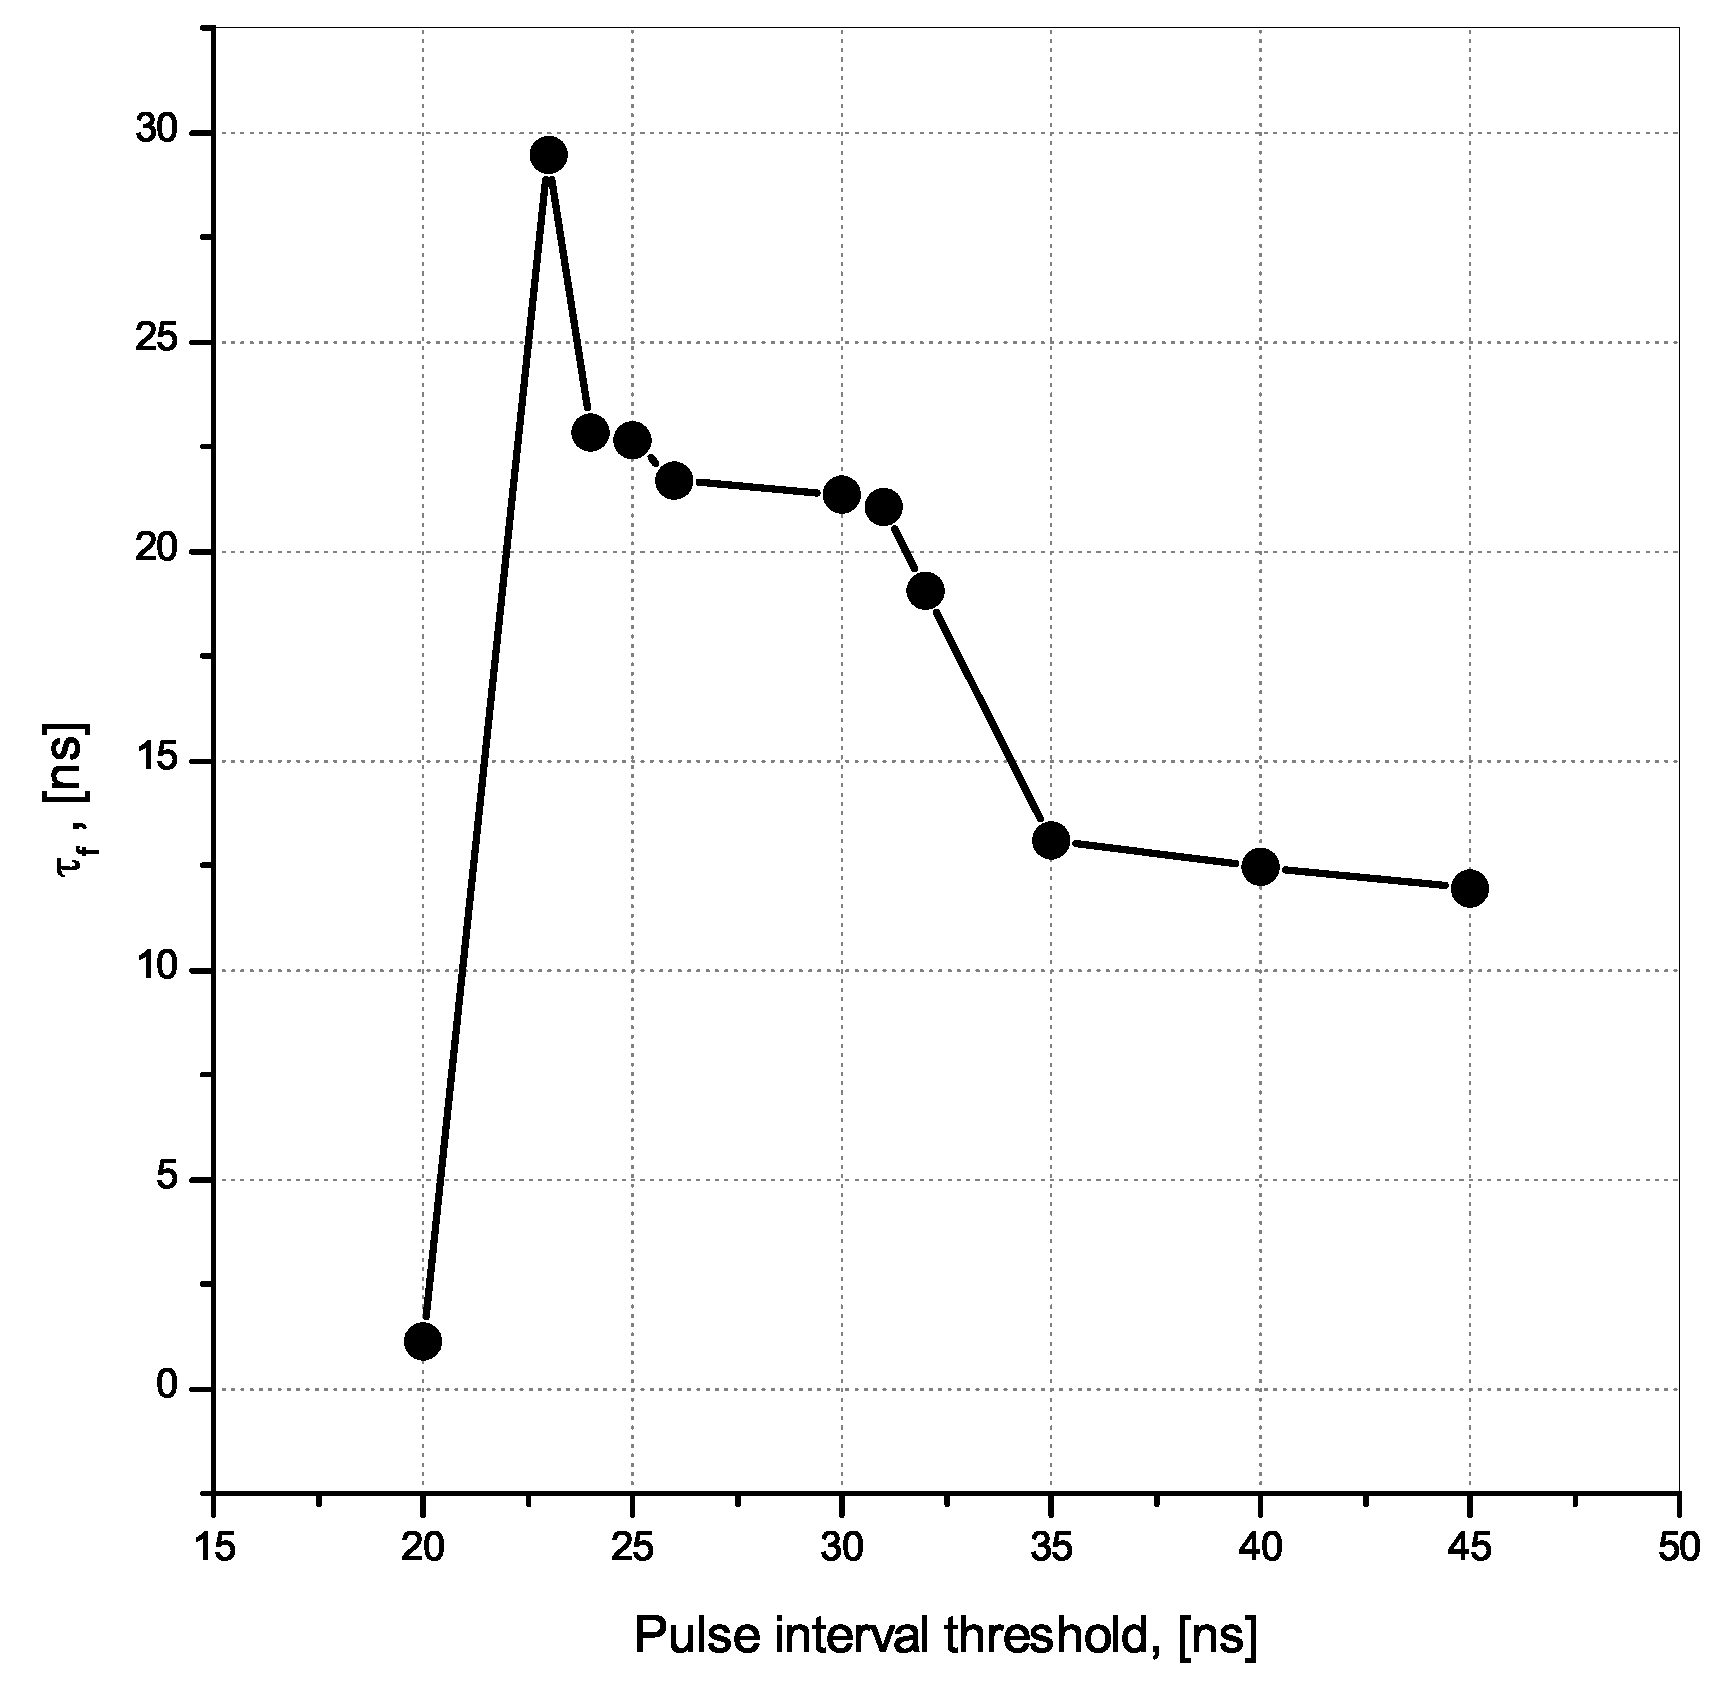
\includegraphics[width=0.47\textwidth]{Hamamatsu_S10362-11-100C_295K_1_OV_dt_spectrum_timecut_eng}
\\
\parbox[t]{0.47\textwidth}{\caption{The pulse interval spectrum approximated by Eq.(\ref{eq:dt_probability_fast_slow}).
Events with cross-talk are not taken into account.
The signal was obtained from Hamamatsu S10362-11-100C at 1V overvoltage and 295K temperature.}
\label{image:Hamamatsu_S10362-11-100C_295K_1_OV_dt_spectrum}}
\hfill
\parbox[t]{0.47\textwidth}{\caption{The dependence of the after-pulse fast component from the pulse interval threshold.
The signal was obtained from Hamamatsu S10362-11-100C at 1V overvoltage and 295K temperature.}
\label{image:Hamamatsu_S10362-11-100C 295K_1_OV_dt_spectrum_timecut}}
\end{figure}

\section{Results}
\subsection{Dark noise}
As the result of the approximation of the pulse interval spectrum the dependence of dark noise rate on a temperature and an overvoltage were obtained (Fig.\ref{image:Hamamatsu_S10362-11-100C_dc_vs_T}, \ref{image:Hamamatsu_S10362-11-100C_dc_vs_V}, \ref{image:Hamamatsu_S13360-3050CS_dc_vs_V_rus}, \ref{image:KETEK_PM1125NS_SB0_dc_vs_V_rus}).
The dependence of dark noise rate on a temperature is expressed by the following formula \cite{Characterization of SiPM: temperature dependencies}:
\begin{eqnarray}\label{eq:Hz_vs_temperature}
\nu(\Delta V = const, T) = A \cdot T^{3/2} \cdot \exp\left[ - \frac{E_g}{2 k_B \cdot T} \right],
\end{eqnarray}
where $A$ is a constant, depending on a voltage, the material and technological parameters, T is an absolute temperature, $E_g$ is a bandgap, $k_B$ is the Boltzmann constant.
The dependence of dark noise rate on an overvoltage is expressed by the linear law:
\begin{eqnarray}\label{eq:Hz_vs_overvoltage}
\nu(\Delta V, T = const) = k \cdot \Delta V
\end{eqnarray}


\begin{figure}[h]
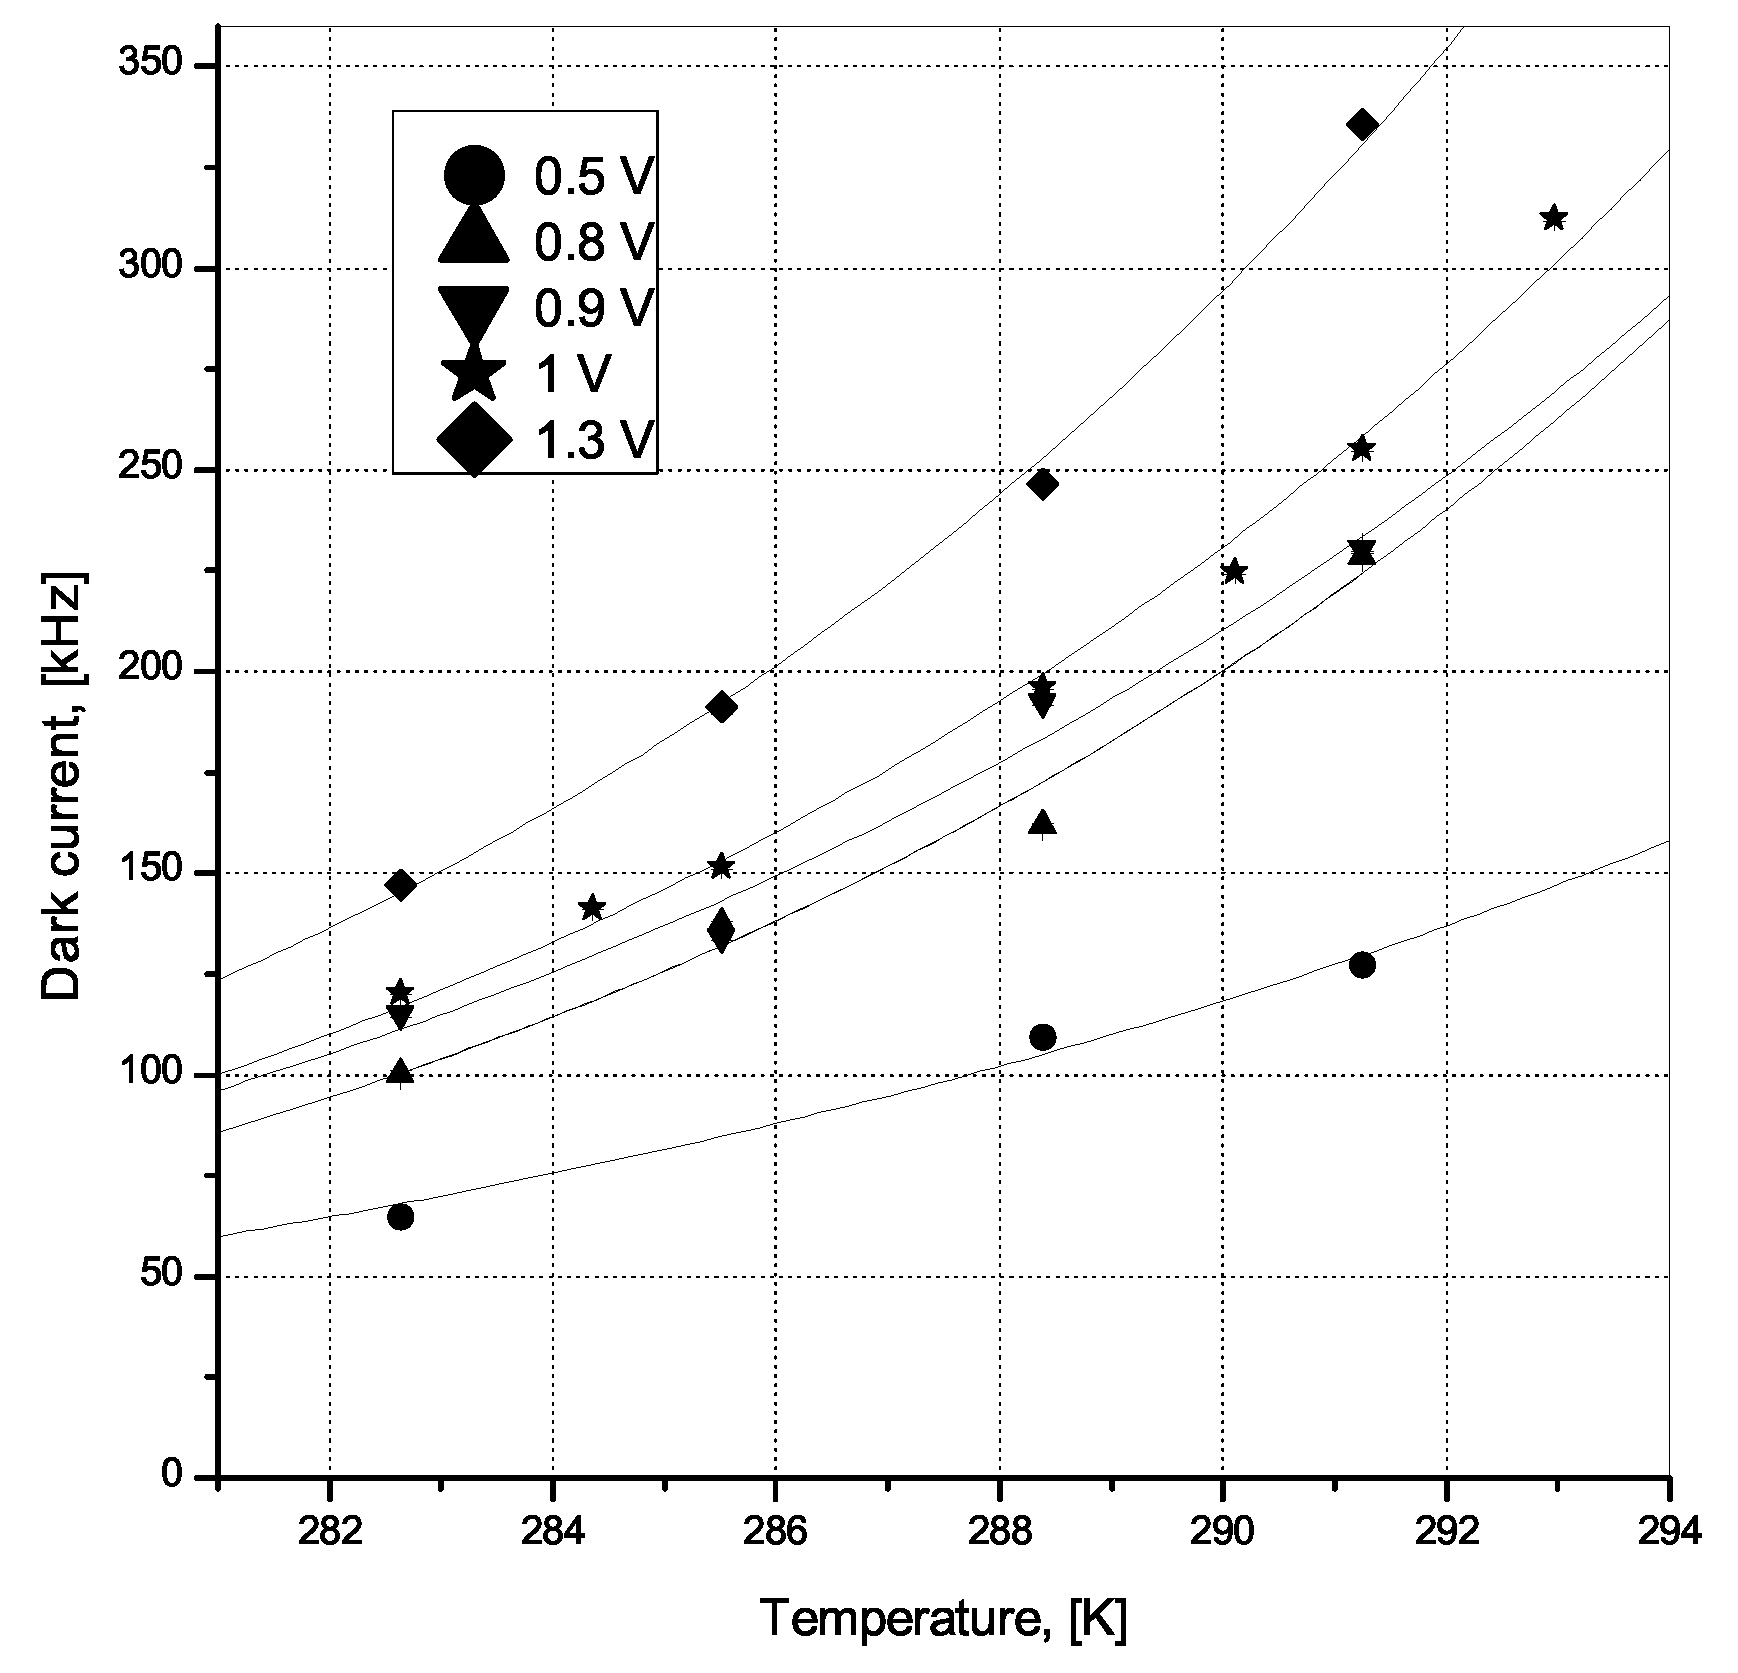
\includegraphics[width=0.47\textwidth]{Hamamatsu_S10362-11-100C_dc_vs_T_eng}
\hfill
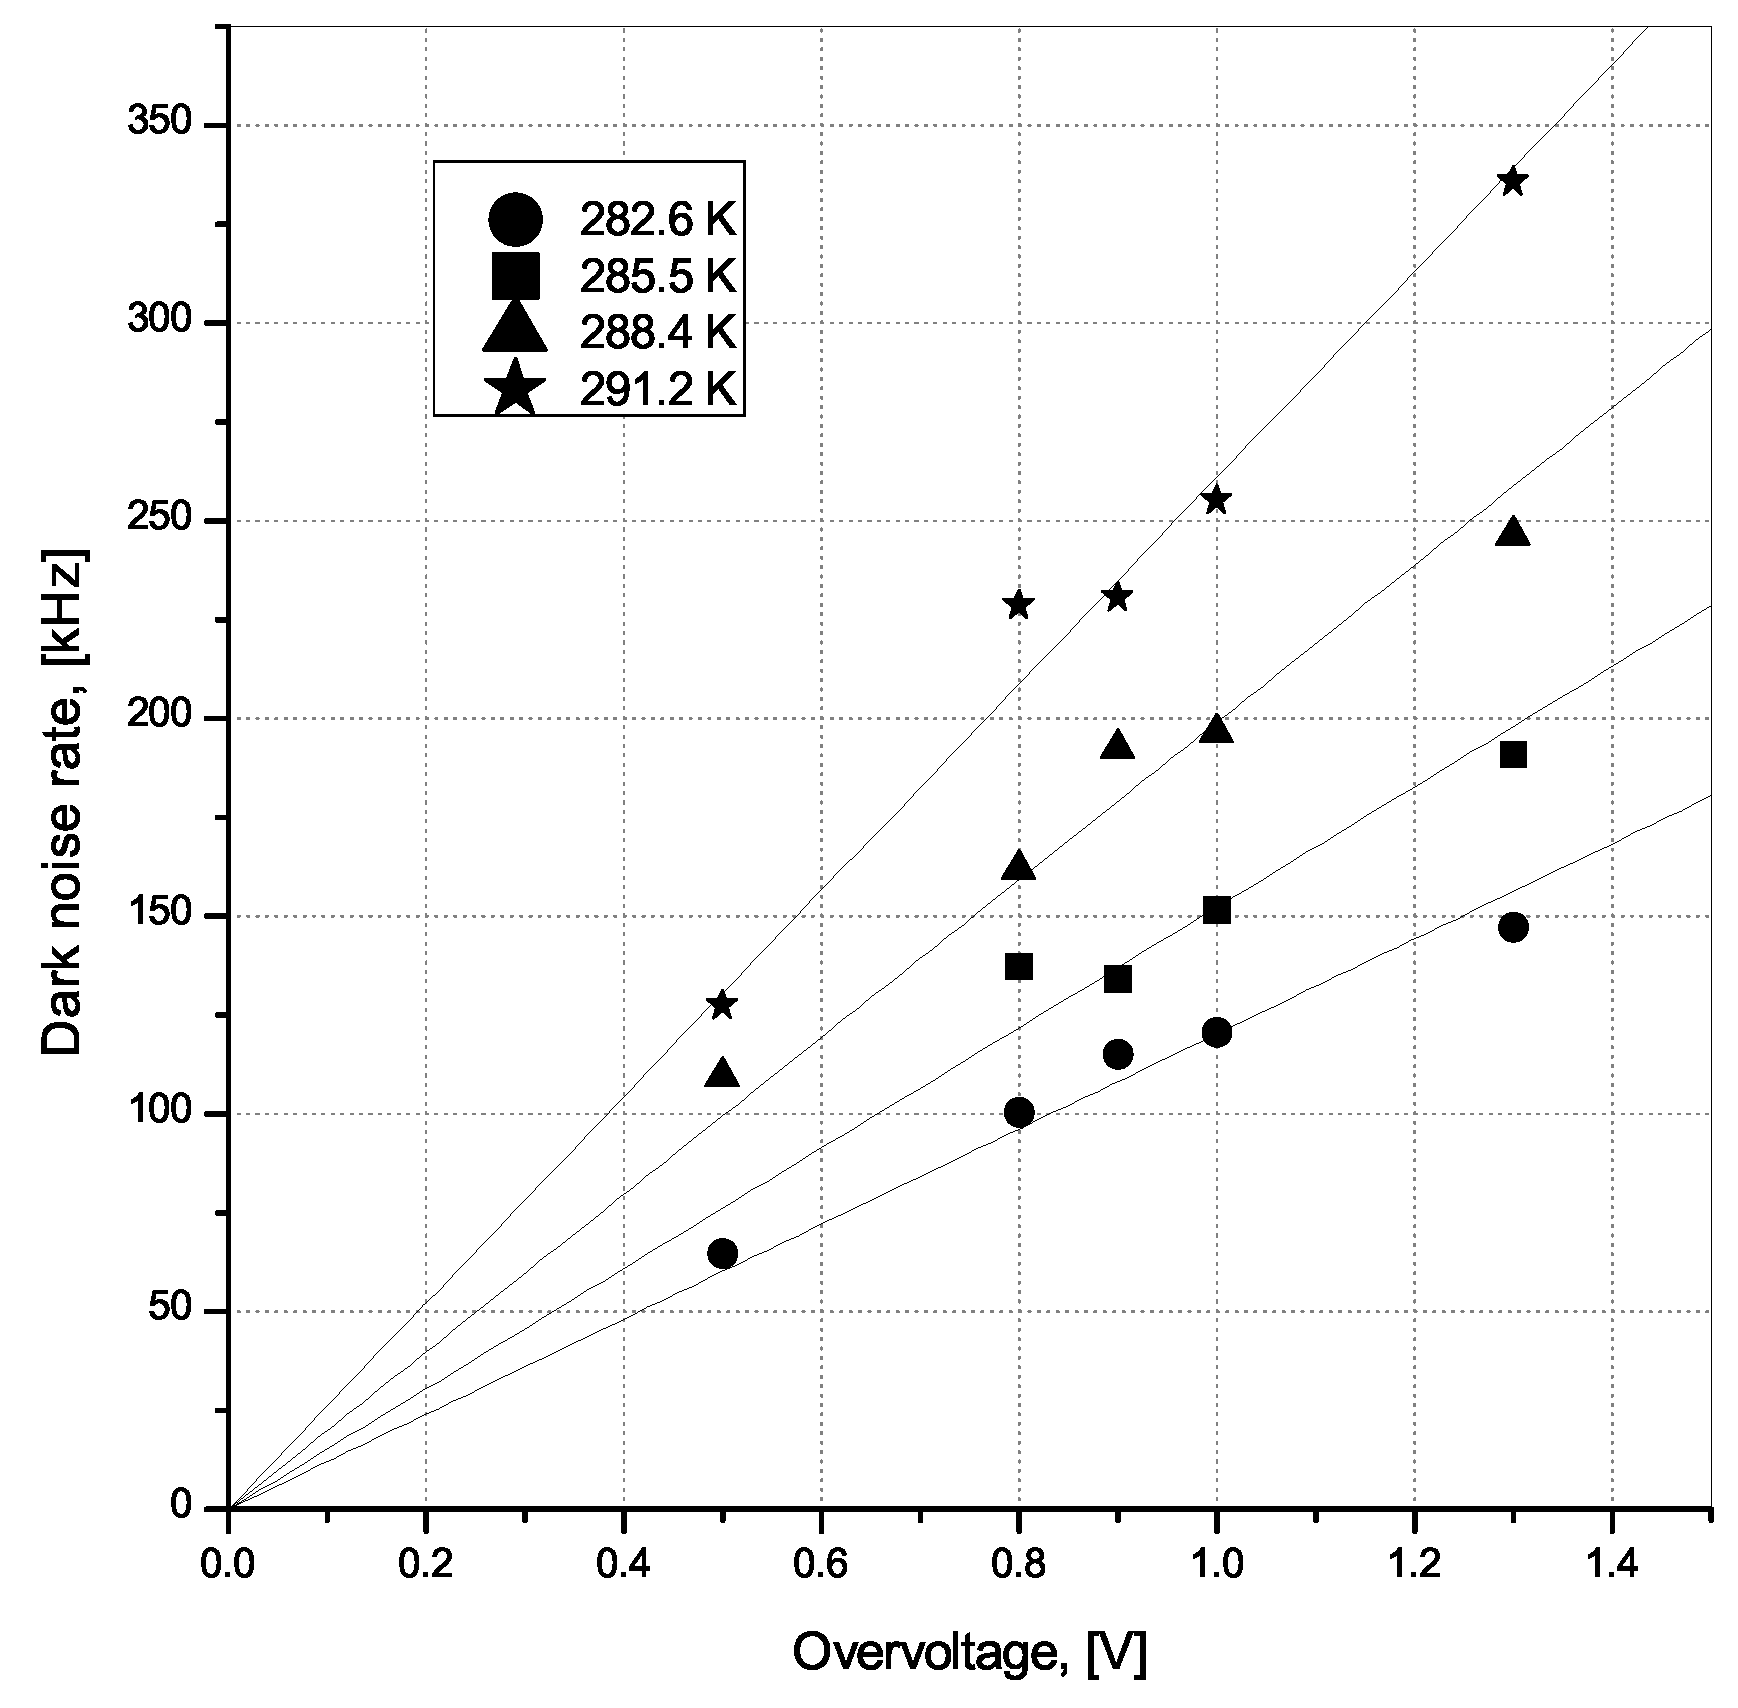
\includegraphics[width=0.47\textwidth]{Hamamatsu_S10362-11-100C_dc_vs_V_eng}
\\
\parbox[t]{0.47\textwidth}{\caption{The dependence of dark noise rate on a temperature at a fixed overvoltage for
Hamamatsu S10362-11-100C. The data were approximated by Eq.(\ref{eq:Hz_vs_temperature}).}
\label{image:Hamamatsu_S10362-11-100C_dc_vs_T}}
\hfill
\parbox[t]{0.47\textwidth}{\caption{The dependence of dark noise rate on a overvoltage at a fixed temperature for
Hamamatsu S10362-11-100C. The data were approximated by Eq.(\ref{eq:Hz_vs_overvoltage}).}
\label{image:Hamamatsu_S10362-11-100C_dc_vs_V}}
\end{figure}

\begin{figure}[h]
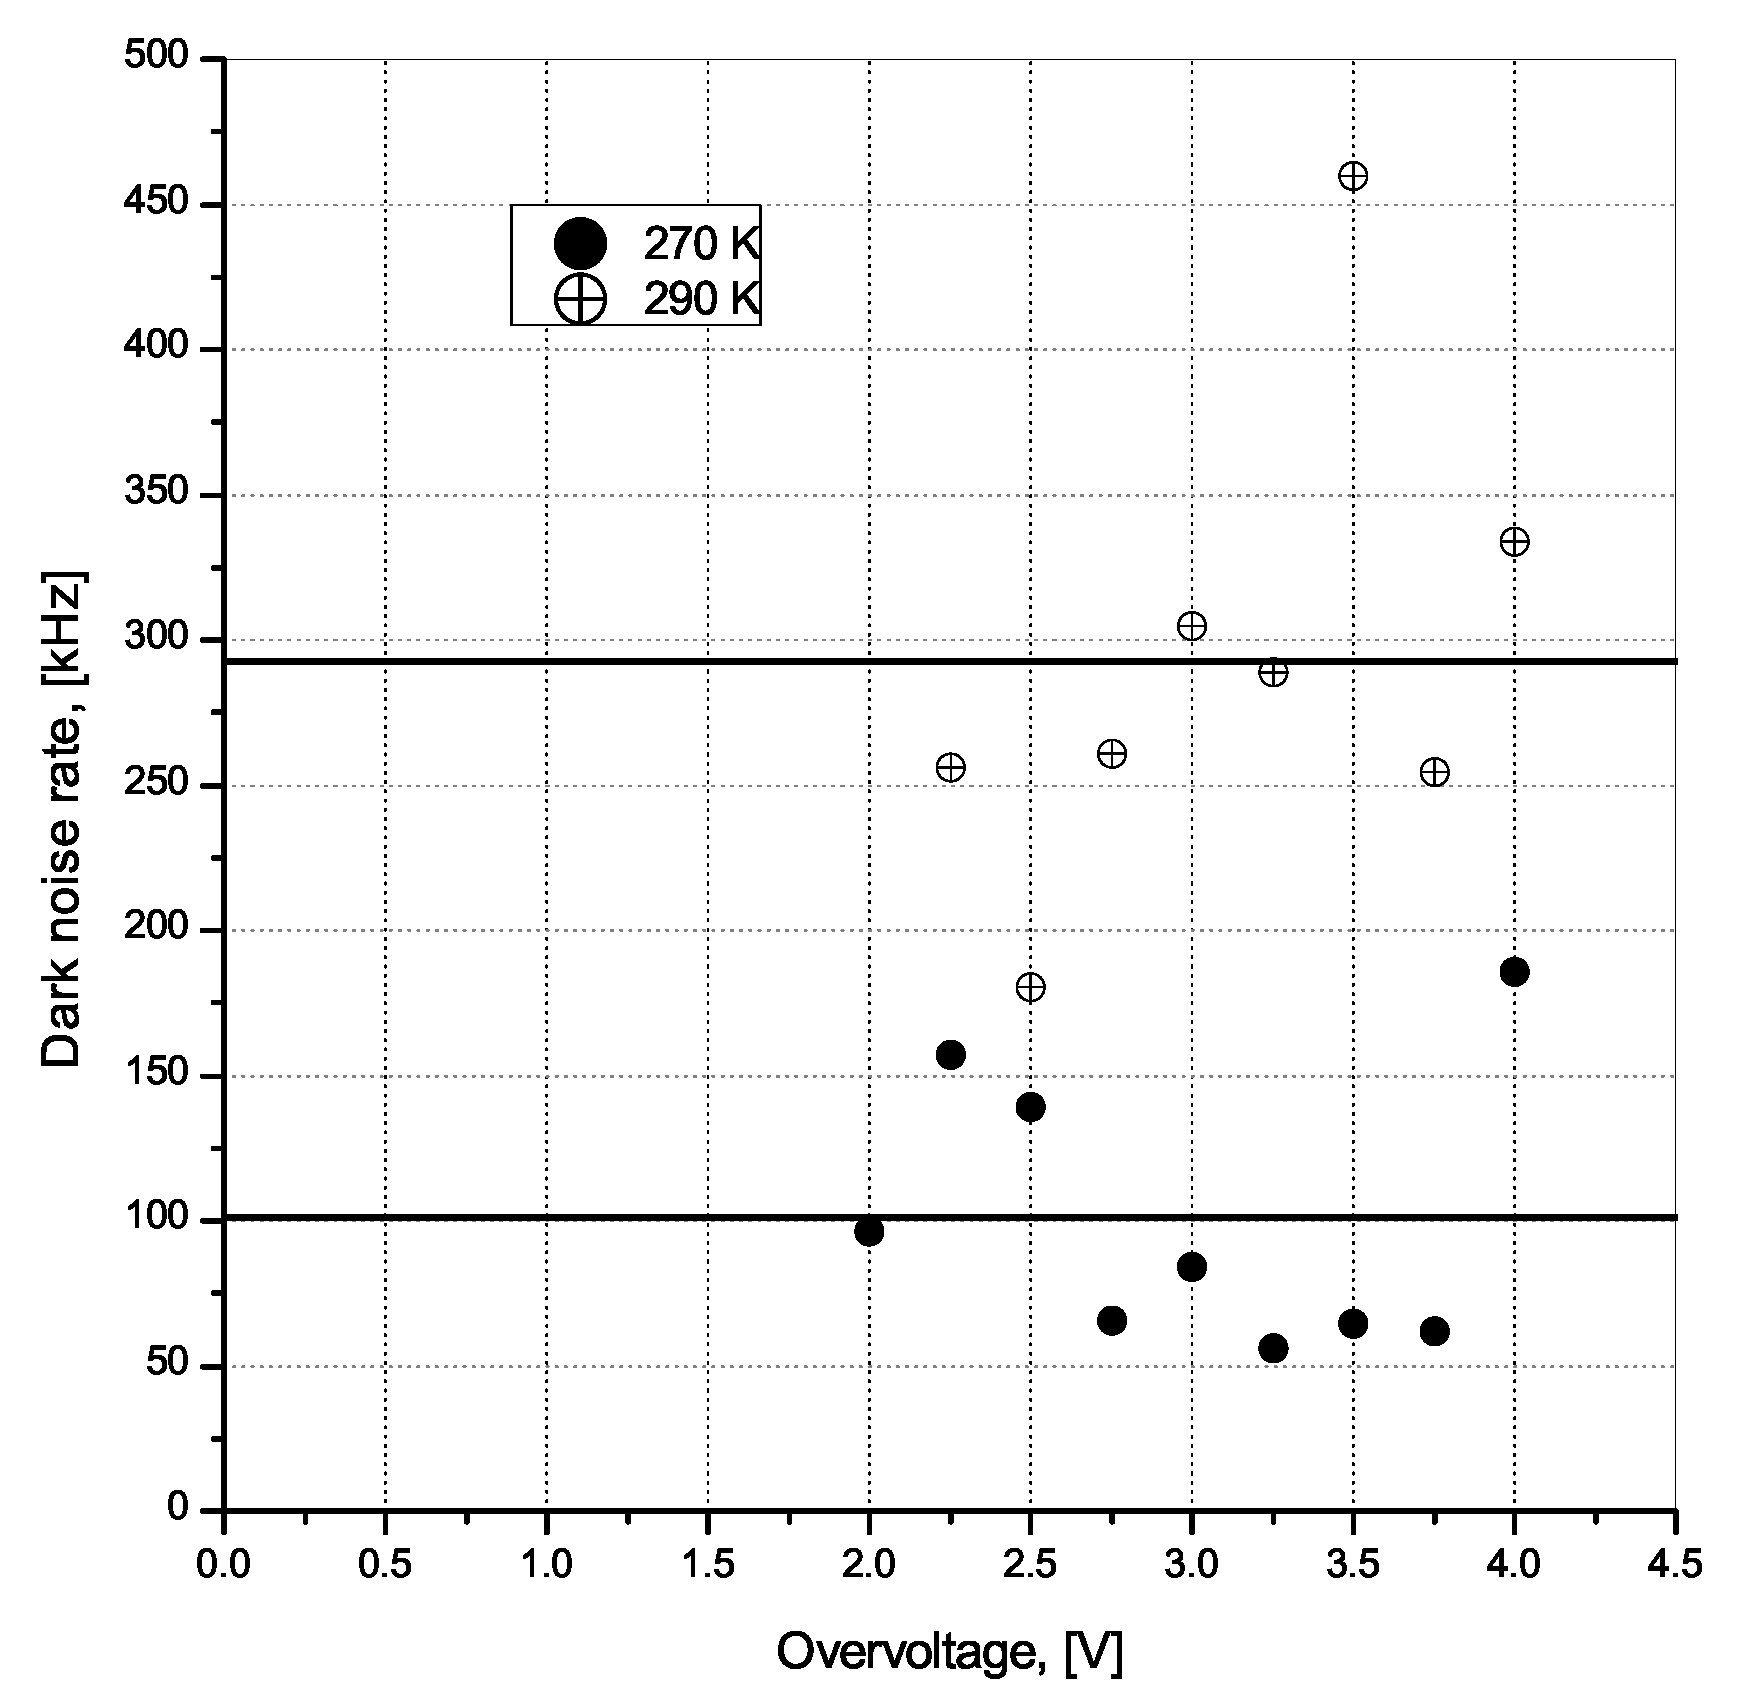
\includegraphics[width=0.47\textwidth]{Hamamatsu_S13360-3050CS_dc_vs_V_eng}
\hfill
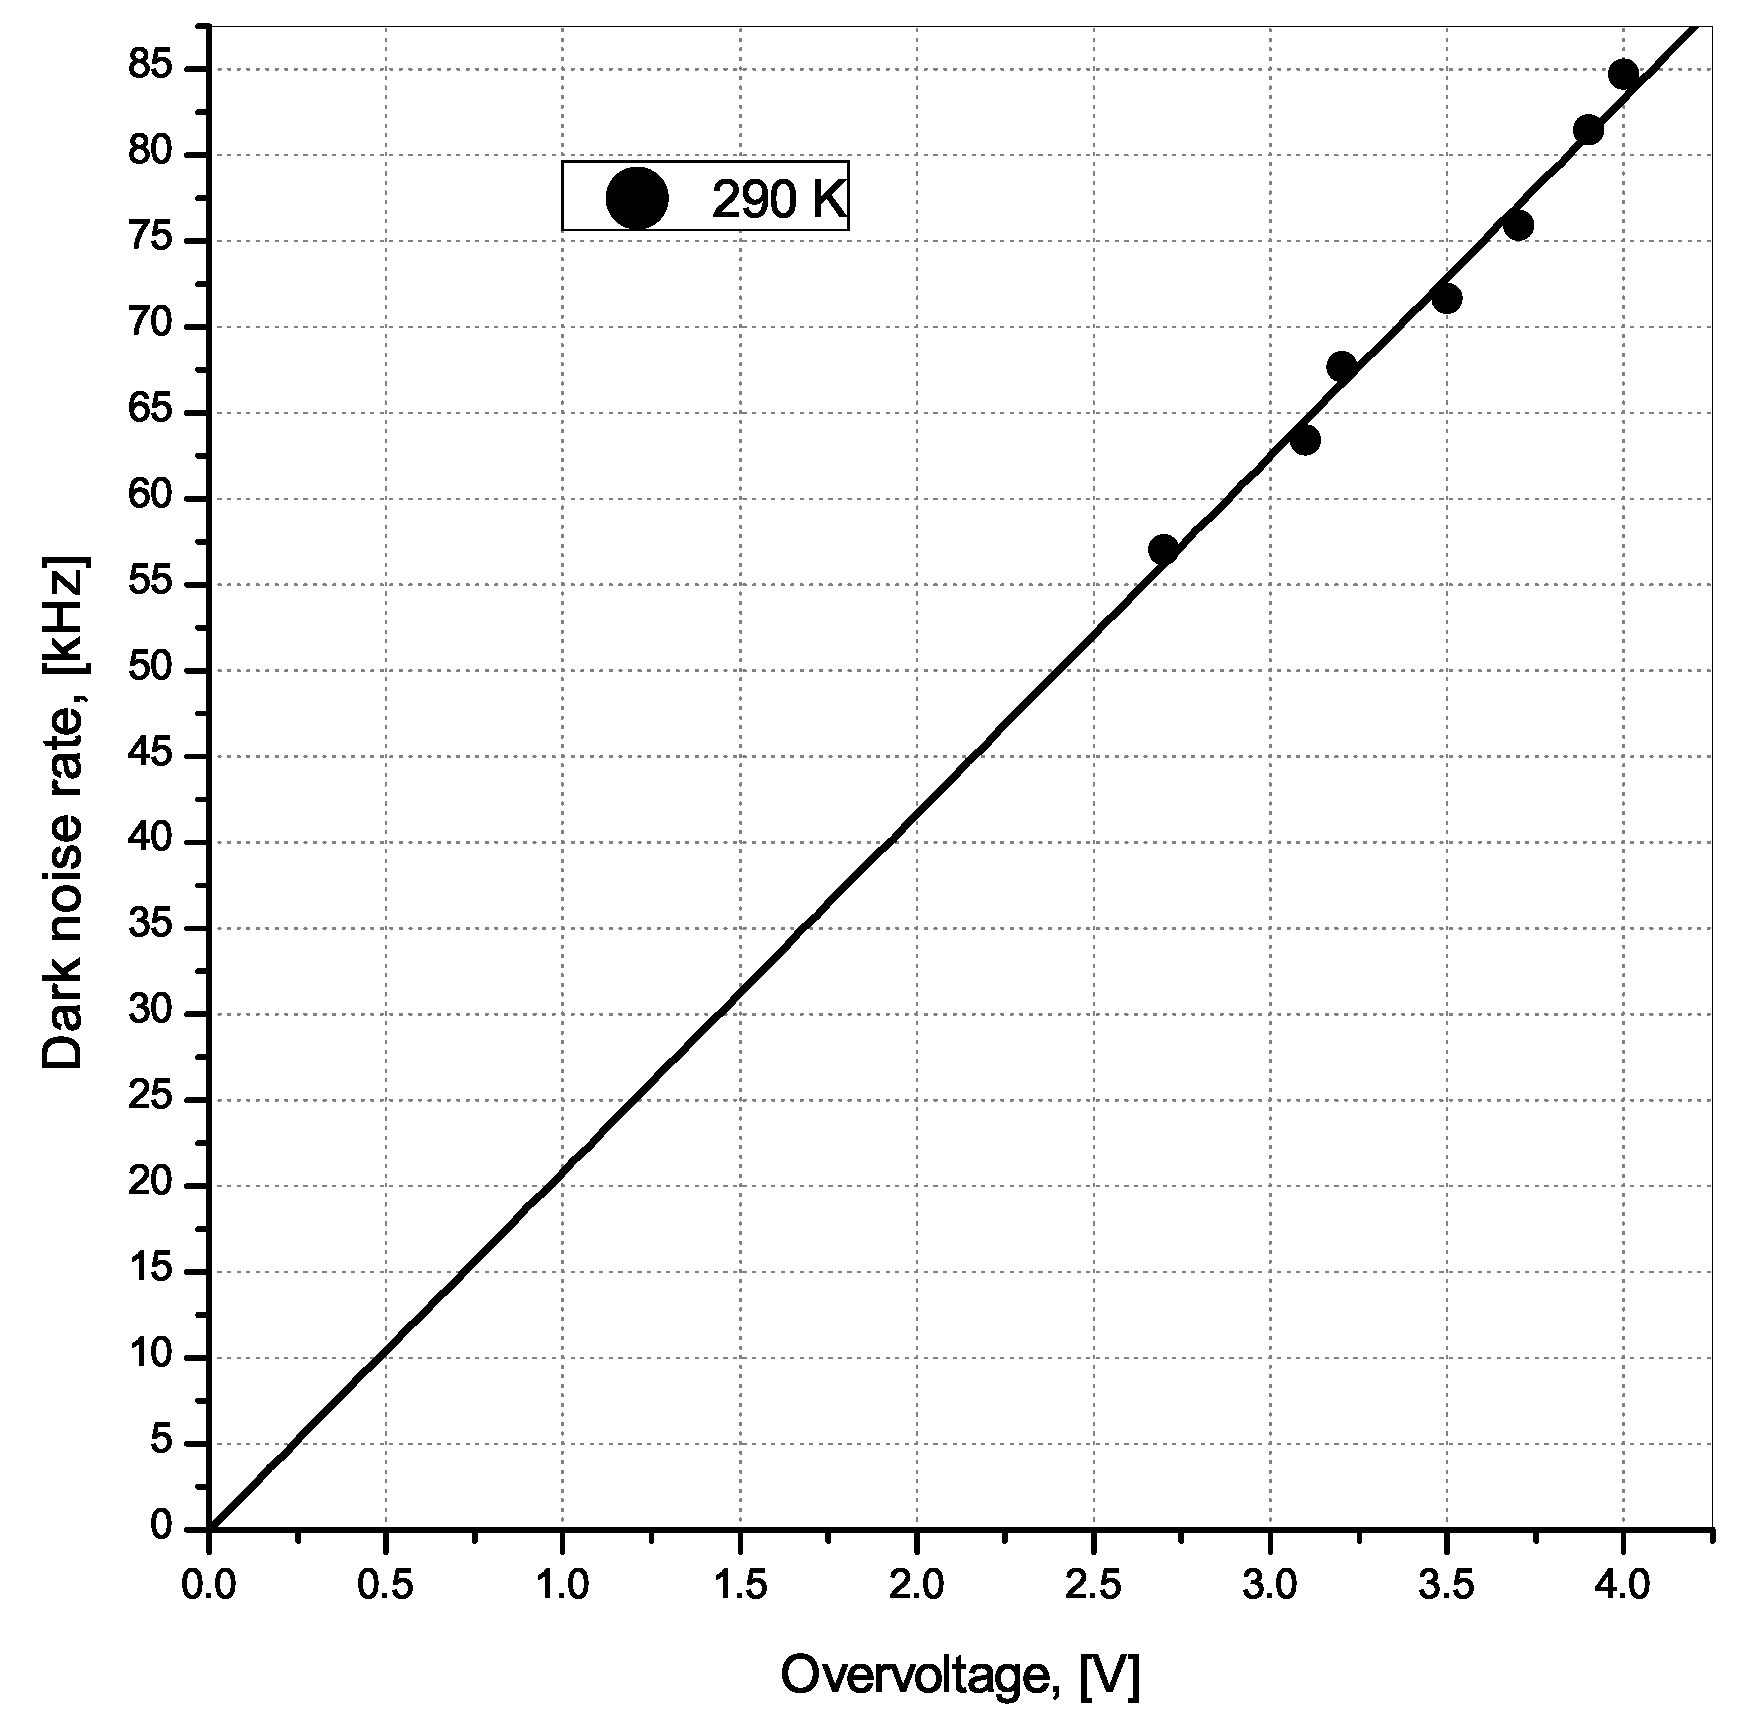
\includegraphics[width=0.47\textwidth]{KETEK_PM1125NS_SB0_dc_vs_V_eng}
\\
\parbox[t]{0.47\textwidth}{\caption{The dependence of dark noise rate on a overvoltage at a fixed temperature for Hamamatsu S13360-3050CS.
Lines are approximation of the data by constant for different temperatures.}
\label{image:Hamamatsu_S13360-3050CS_dc_vs_V_rus}}
\hfill
\parbox[t]{0.47\textwidth}{\caption{The dependence of dark noise rate on a overvoltage at a fixed temperature for KETEK PM1125NS-SB0.
The line is approximation of the data by linear function.}
\label{image:KETEK_PM1125NS_SB0_dc_vs_V_rus}}
\end{figure}


However we were failed to collect enough statistics for data approximation in this manner for Hamamatsu S13360-3050CS because of its low noise level.
For the same reason, only one point at the maximum noise level was obtained for KETEK PM1125NS-SB0.


\subsection{Cross-talk}
The $A_{1}$ cluster (Fig.~\ref{image:Hamamatsu_S10362-11-100C_295K_1V_Chi2_amp 1}) consists of single-electron pulses.
The $B_{1}$ cluster consists of pulses caused by the simultaneous triggering of two cells.
The $C_{1}$ cluster consists of pulses caused by the simultaneous triggering of three cells.
The $A_{2}$ cluster (Fig.~\ref{image:Hamamatsu_S10362-11-100C_295K_1_OV_Chi2_amp1_amp2}) consists of pulses caused by triggering of one cell with the subsequent after-pulse or triggering two cells at different time points because of dark noise.
The $B_{2}$ cluster consists of pulses caused by the simultaneous triggering of two cells with the subsequent after-pulse of one of the cells or triggering of one cell with the subsequent after-pulse, causing cross-talk.

At the moment, we calculate the cross-talk probability as follows:
\begin{eqnarray}\label{eq:xtalk_general}
P_{X-talk} = ( N_{B_{1}} + N_{C_{1}} ) / (N_{A_{1}} + N_{B_{1}} + N_{C_{1}})
\end{eqnarray}
This is an approximate formula because one should take into account the fact that a small part of with cross-talk events is contained in $B_{2}$, $C_{2}$, $B_{3}$, $C_{3}$, etc. clusters.

The cross-talk probability should have the quadratic dependence of an overvoltage in the first approximation.
This is explained by the cross-talk probability $P_{x-talk}$ is proportional to the number of electrons in the avalanche $G$ and the triggering probability of cells by photon $\varepsilon_{Geiger}$.
$G$ and $\varepsilon_{Geiger}$ have a linear dependence on an overvoltage(for $\varepsilon_{Geiger}$ value the dependence differs
from linear at a high overvoltage \cite{Measurement of PDE of MPPC with different wavelengths of light}):
\begin{eqnarray}\label{eq:xtalk_prob_V2_reason}
P_{x-talk}(\Delta V) \propto  G(\Delta V) \cdot \varepsilon_{Geiger}(\Delta V)
\end{eqnarray}

Thus, the experimental data were approximated by the following formula:
\begin{eqnarray}\label{eq:xtalk_vs_T_V}
P_{x-talk}(\Delta V, T) = k_{x-talk} \cdot \Delta V^2
\end{eqnarray}

The results of processing are shown on Fig. \ref{image:Hamamatsu_S10362-11-100C_xtalk_vs_T}, \ref{image:Hamamatsu_S10362-11-100C_xtalk_vs_V}, \ref{image:Hamamatsu_S13360-3050CS_xtalk_vs_V_rus}, \ref{image:KETEK_PM1125NS_SB0_x-tlak_vs_V_rus}.

\begin{figure}[h]
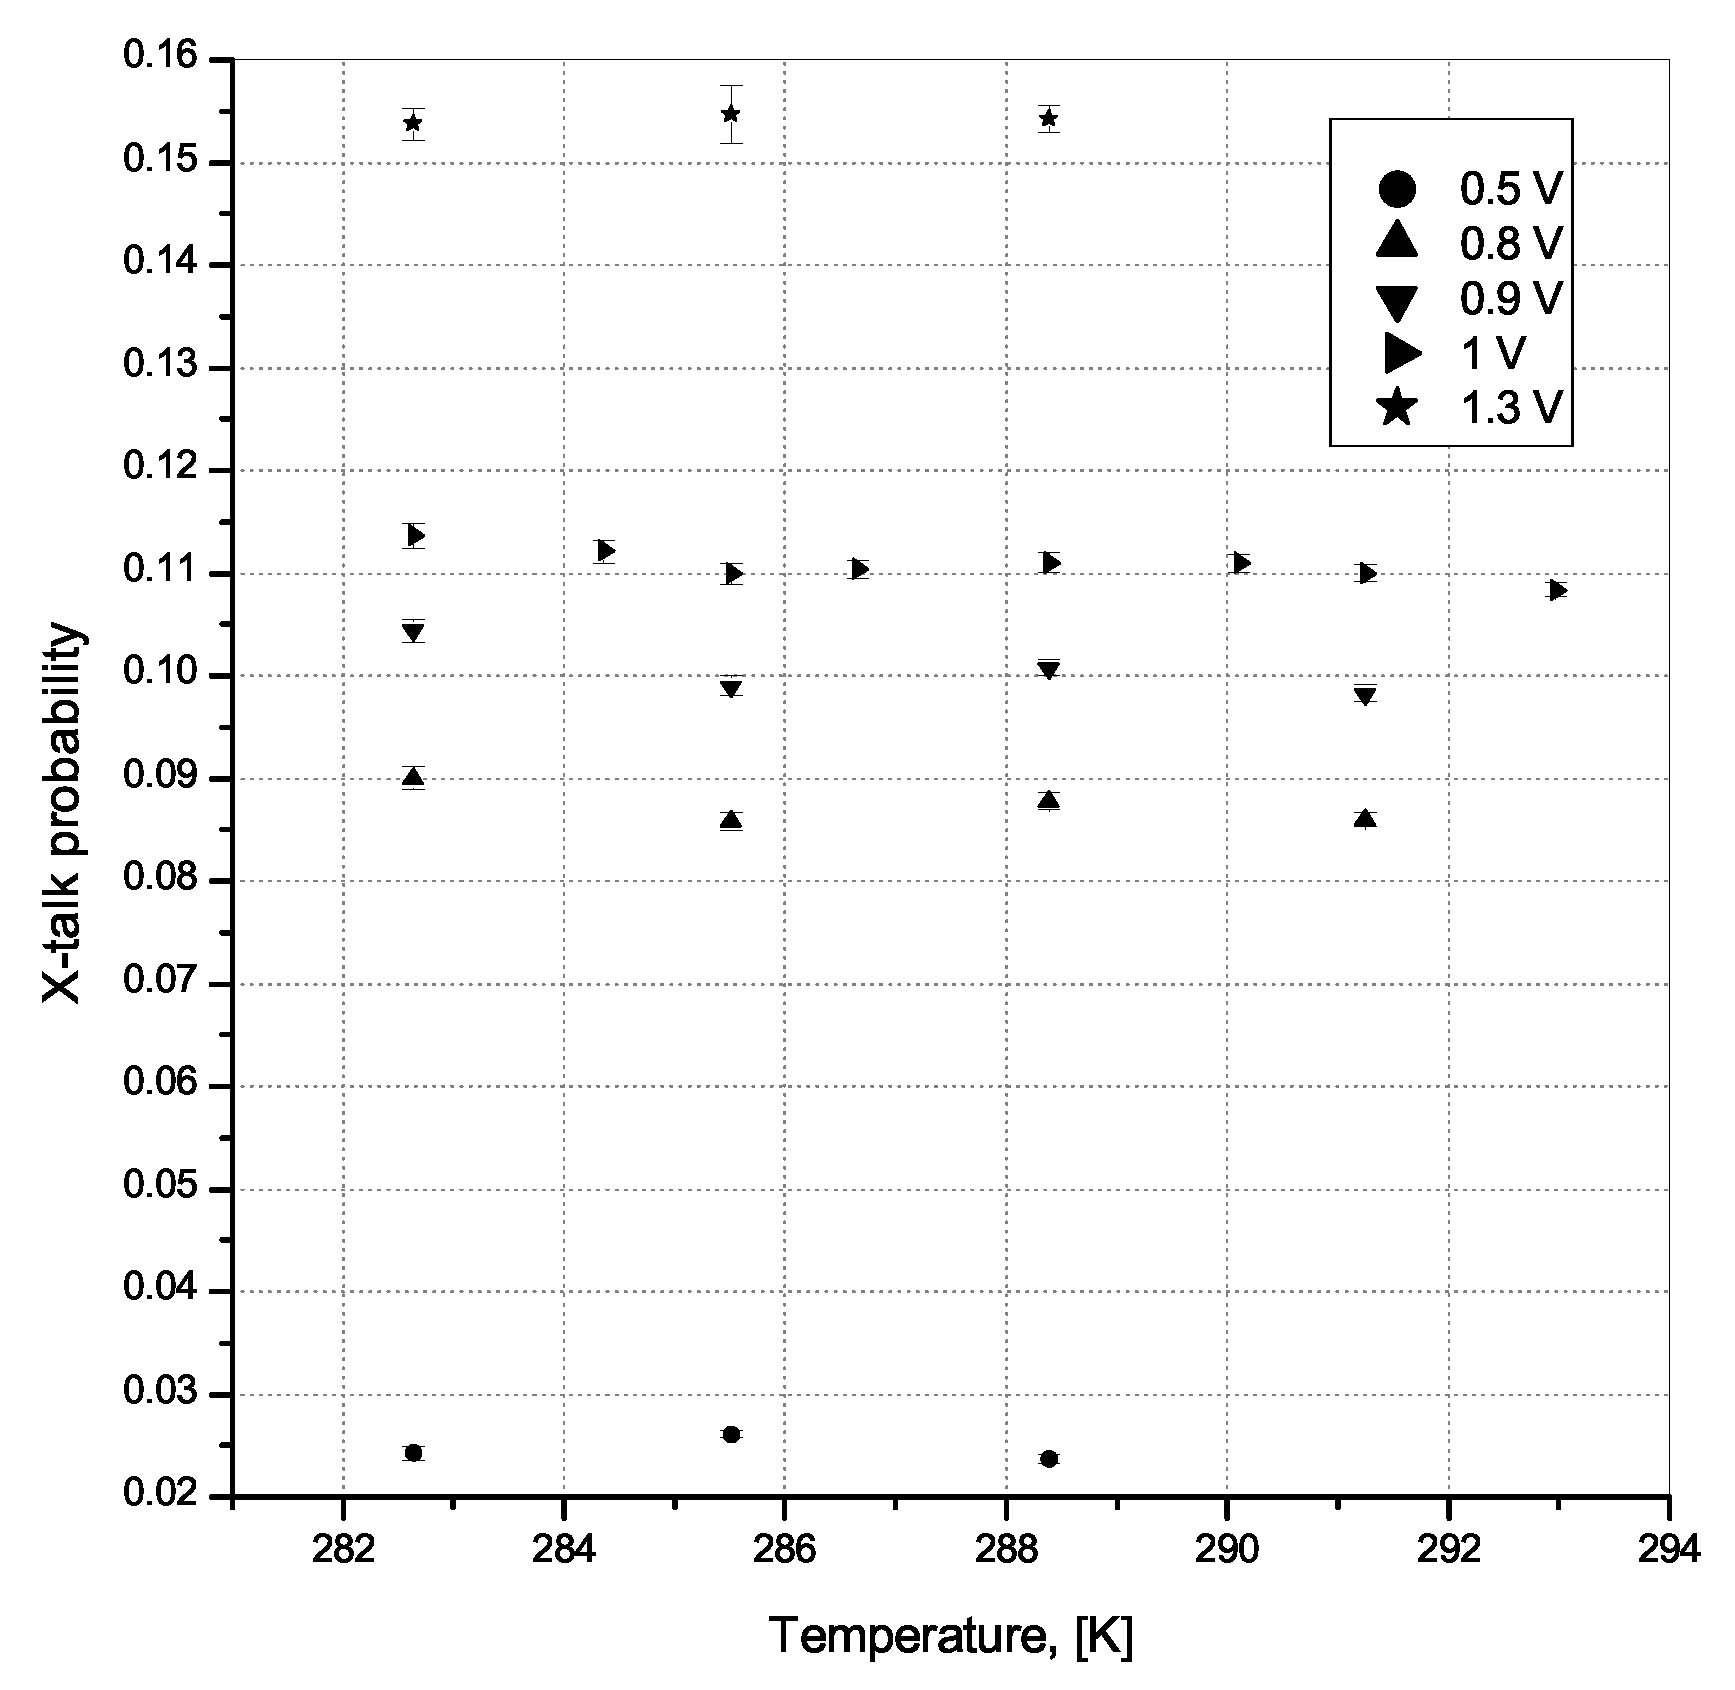
\includegraphics[width=0.47\textwidth]{Hamamatsu_S10362-11-100C_xtalk_vs_T_eng}
\hfill
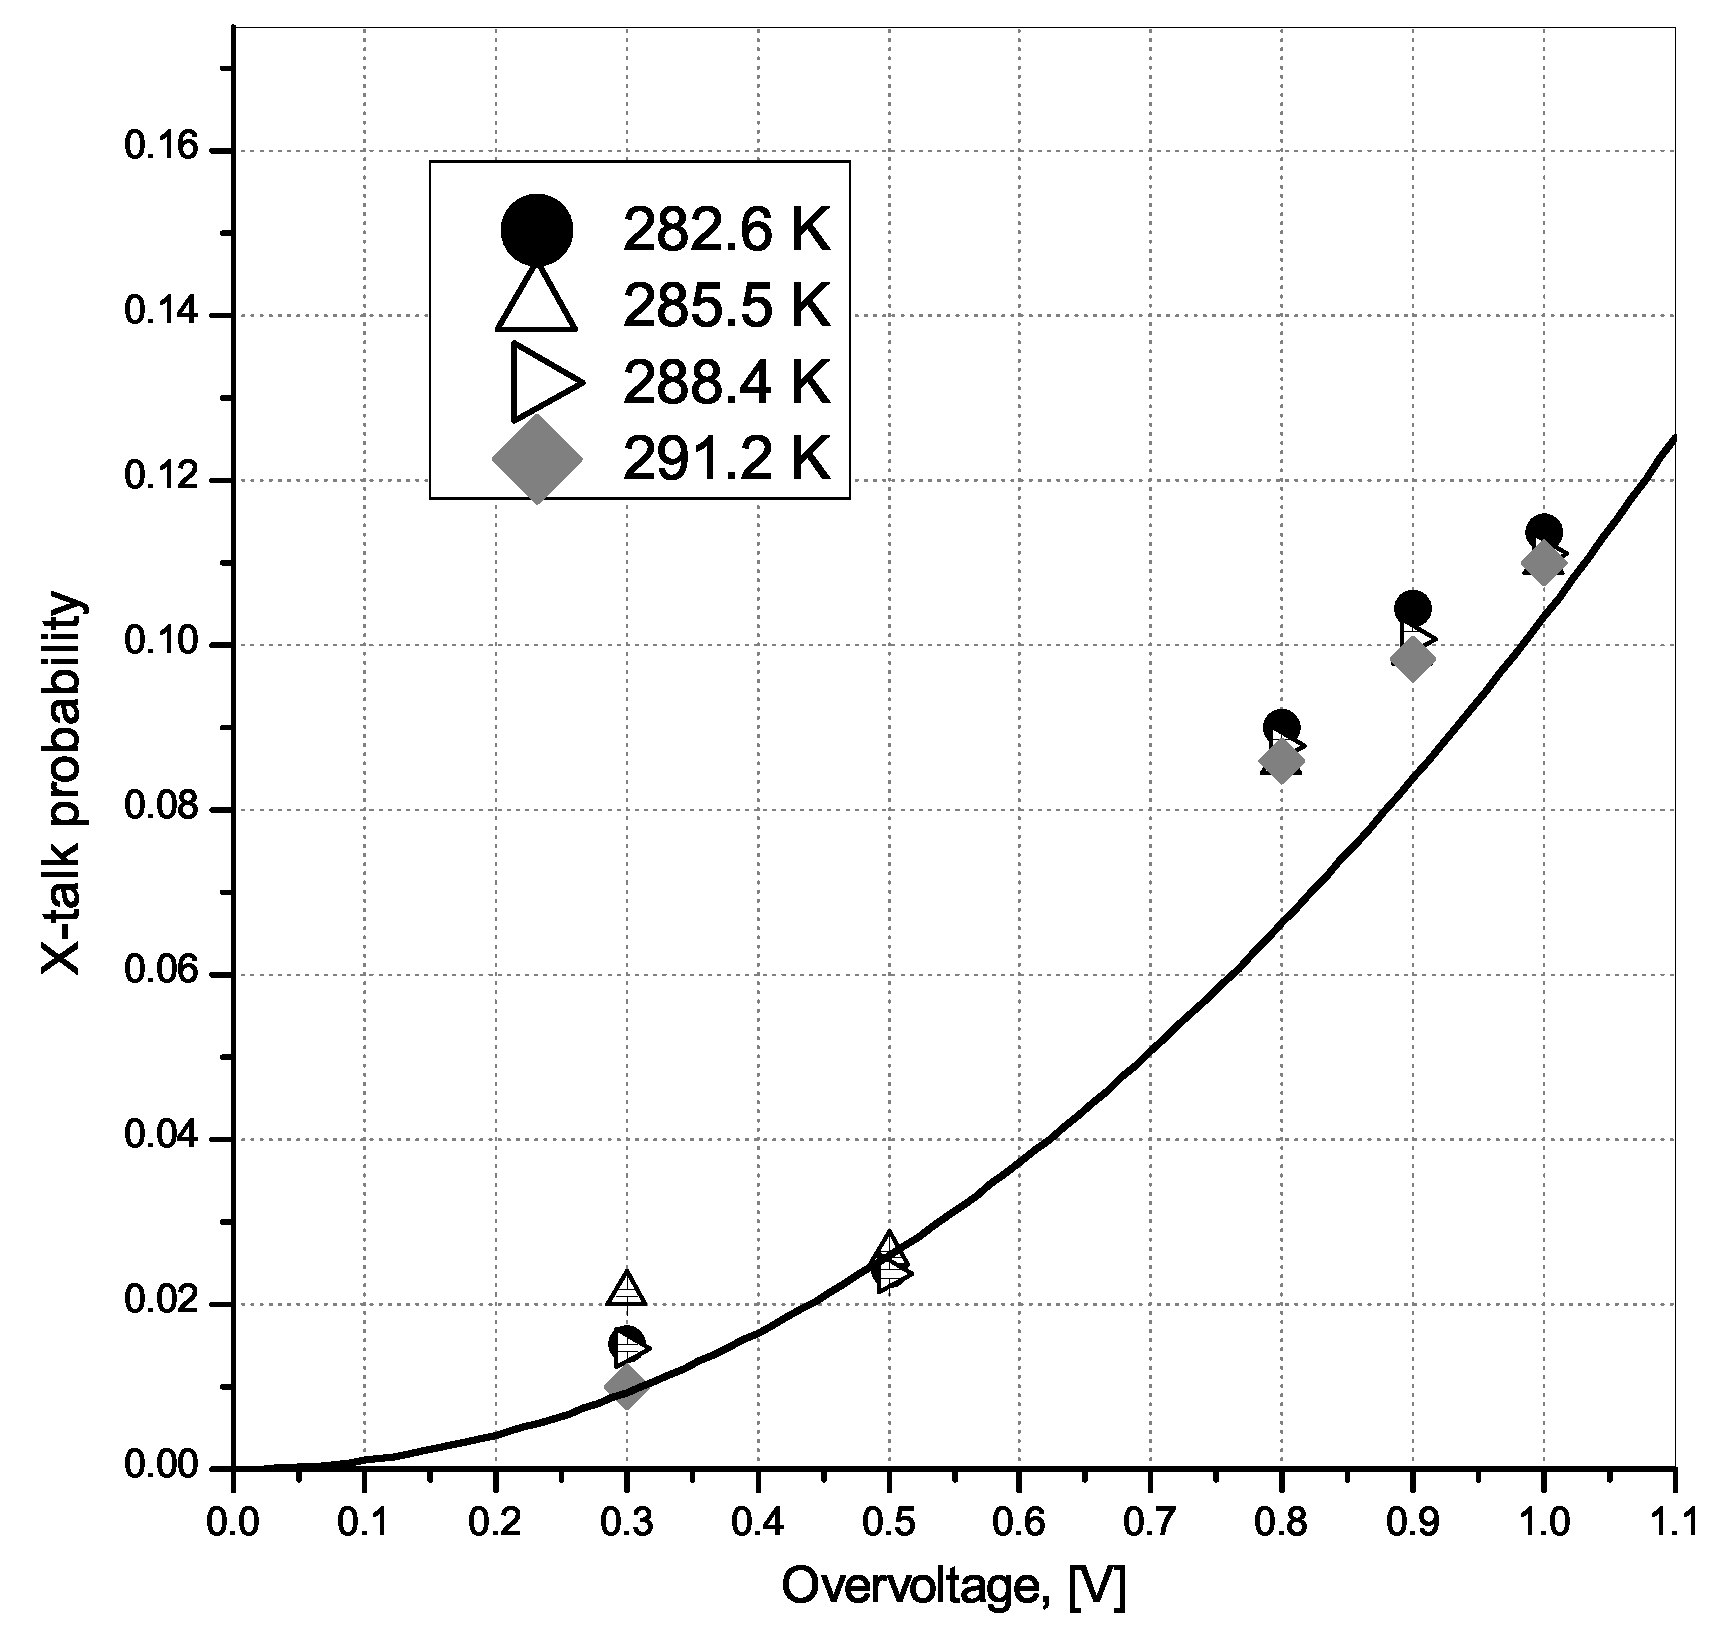
\includegraphics[width=0.47\textwidth]{Hamamatsu_S10362-11-100C_xtalk_vs_V_eng}
\\
\parbox[t]{0.47\textwidth}{\caption{The dependence of the cross-talk probability on a temperature at a fixed overvoltage for Hamamatsu S10362-11-100C.}
\label{image:Hamamatsu_S10362-11-100C_xtalk_vs_T}}
\hfill
\parbox[t]{0.47\textwidth}{\caption{The dependence of the cross-talk probability on a overvoltage at a fixed temperature for
Hamamatsu S10362-11-100C. The data were approximated by a quadratic function.}
\label{image:Hamamatsu_S10362-11-100C_xtalk_vs_V}}
\end{figure}

\begin{figure}[h]
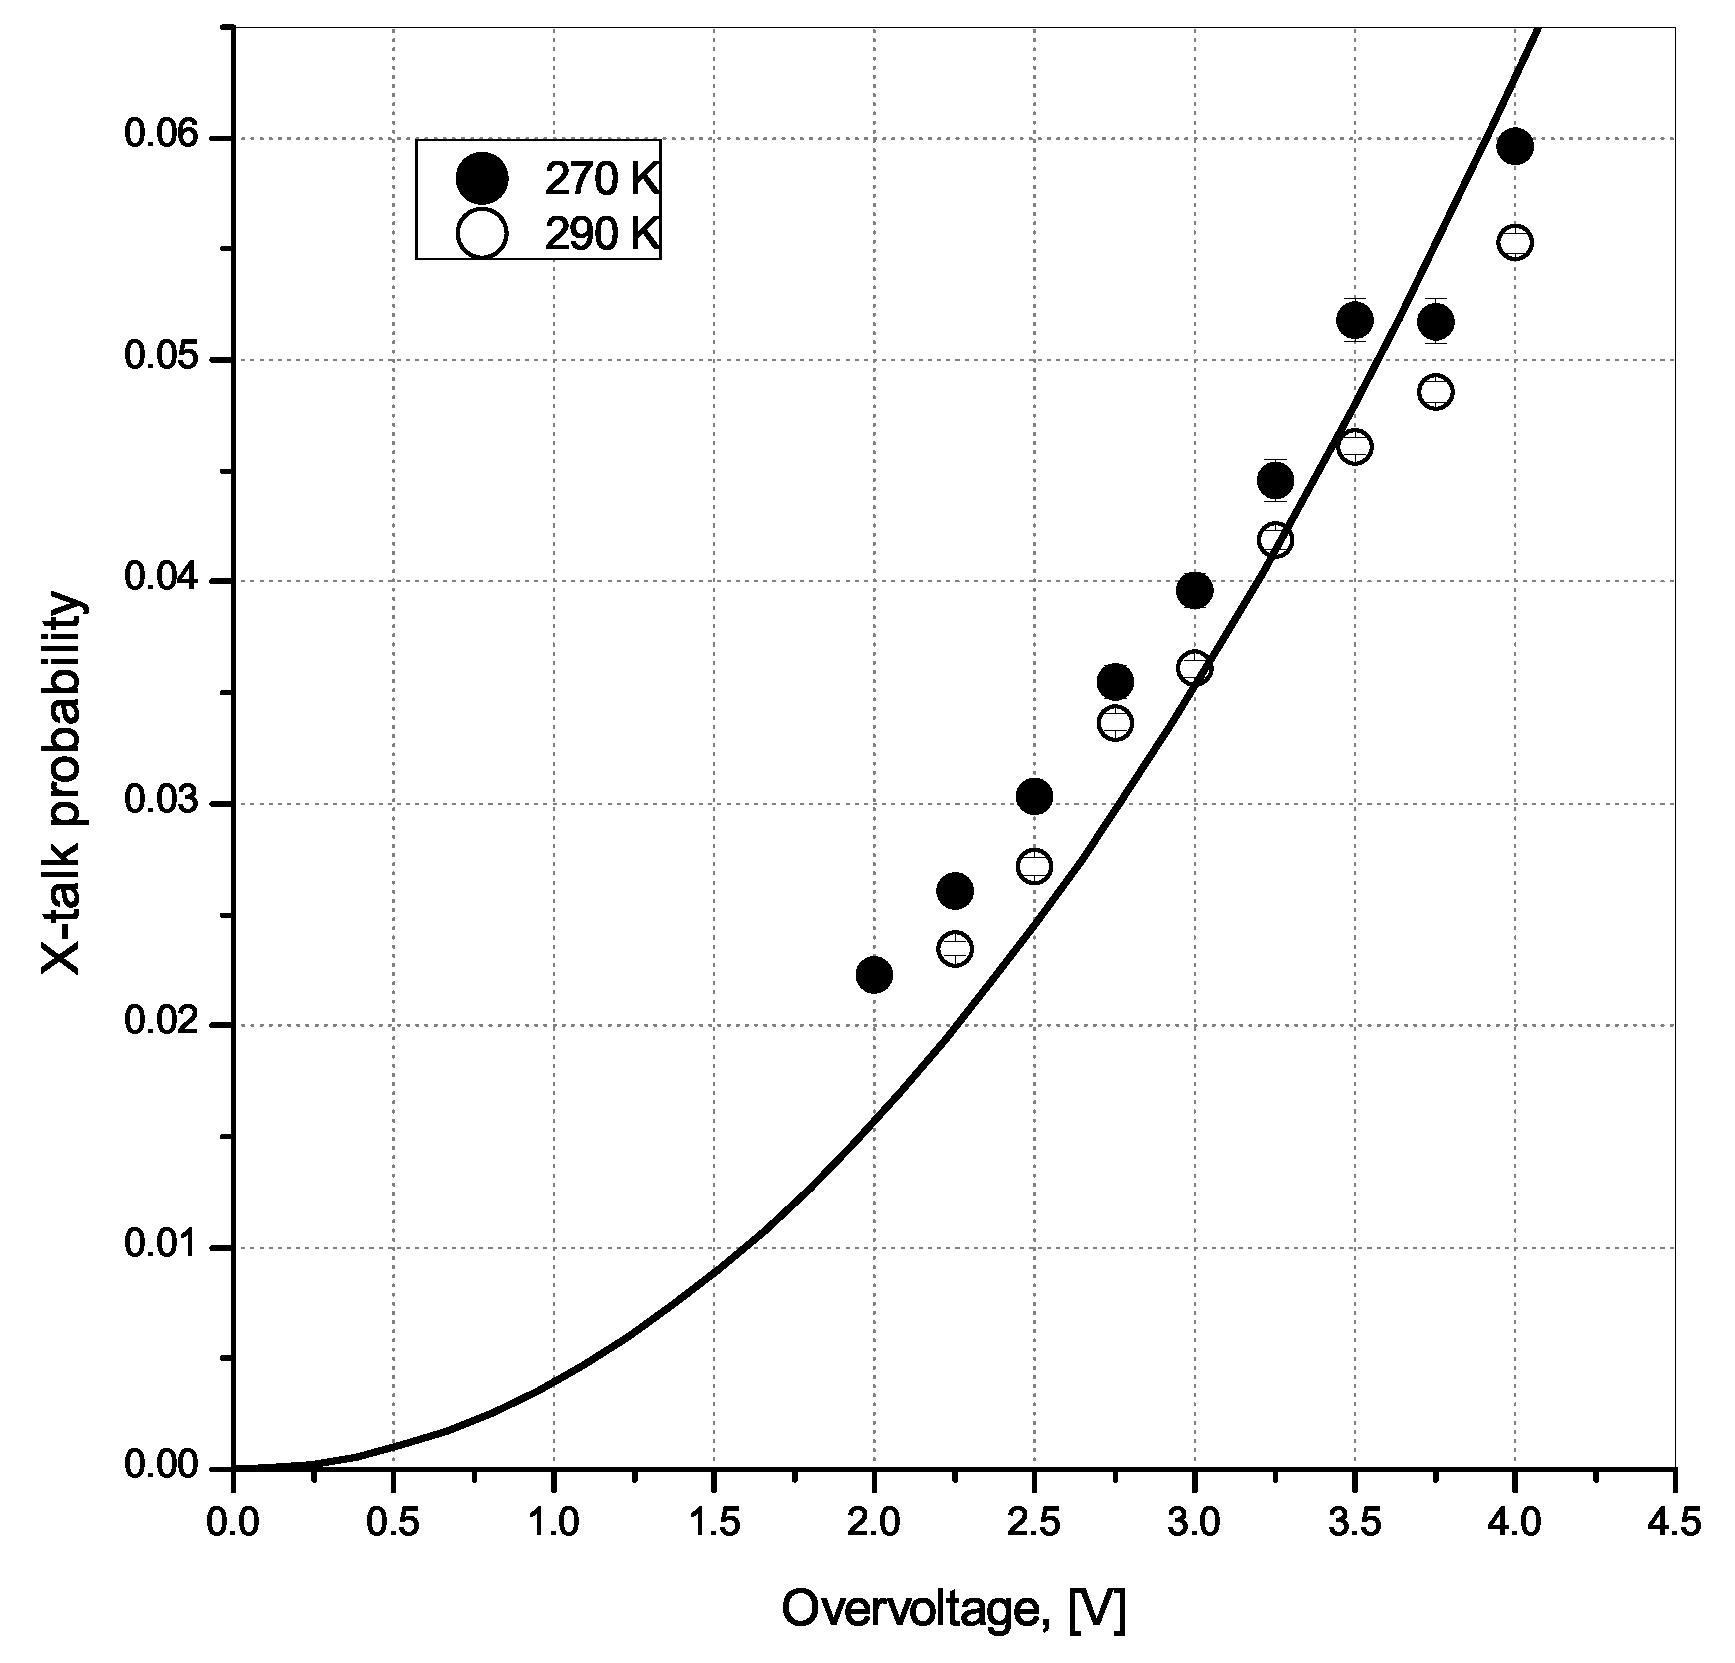
\includegraphics[width=0.47\textwidth]{Hamamatsu_S13360-3050CS_xtalk_vs_V_eng}
\hfill
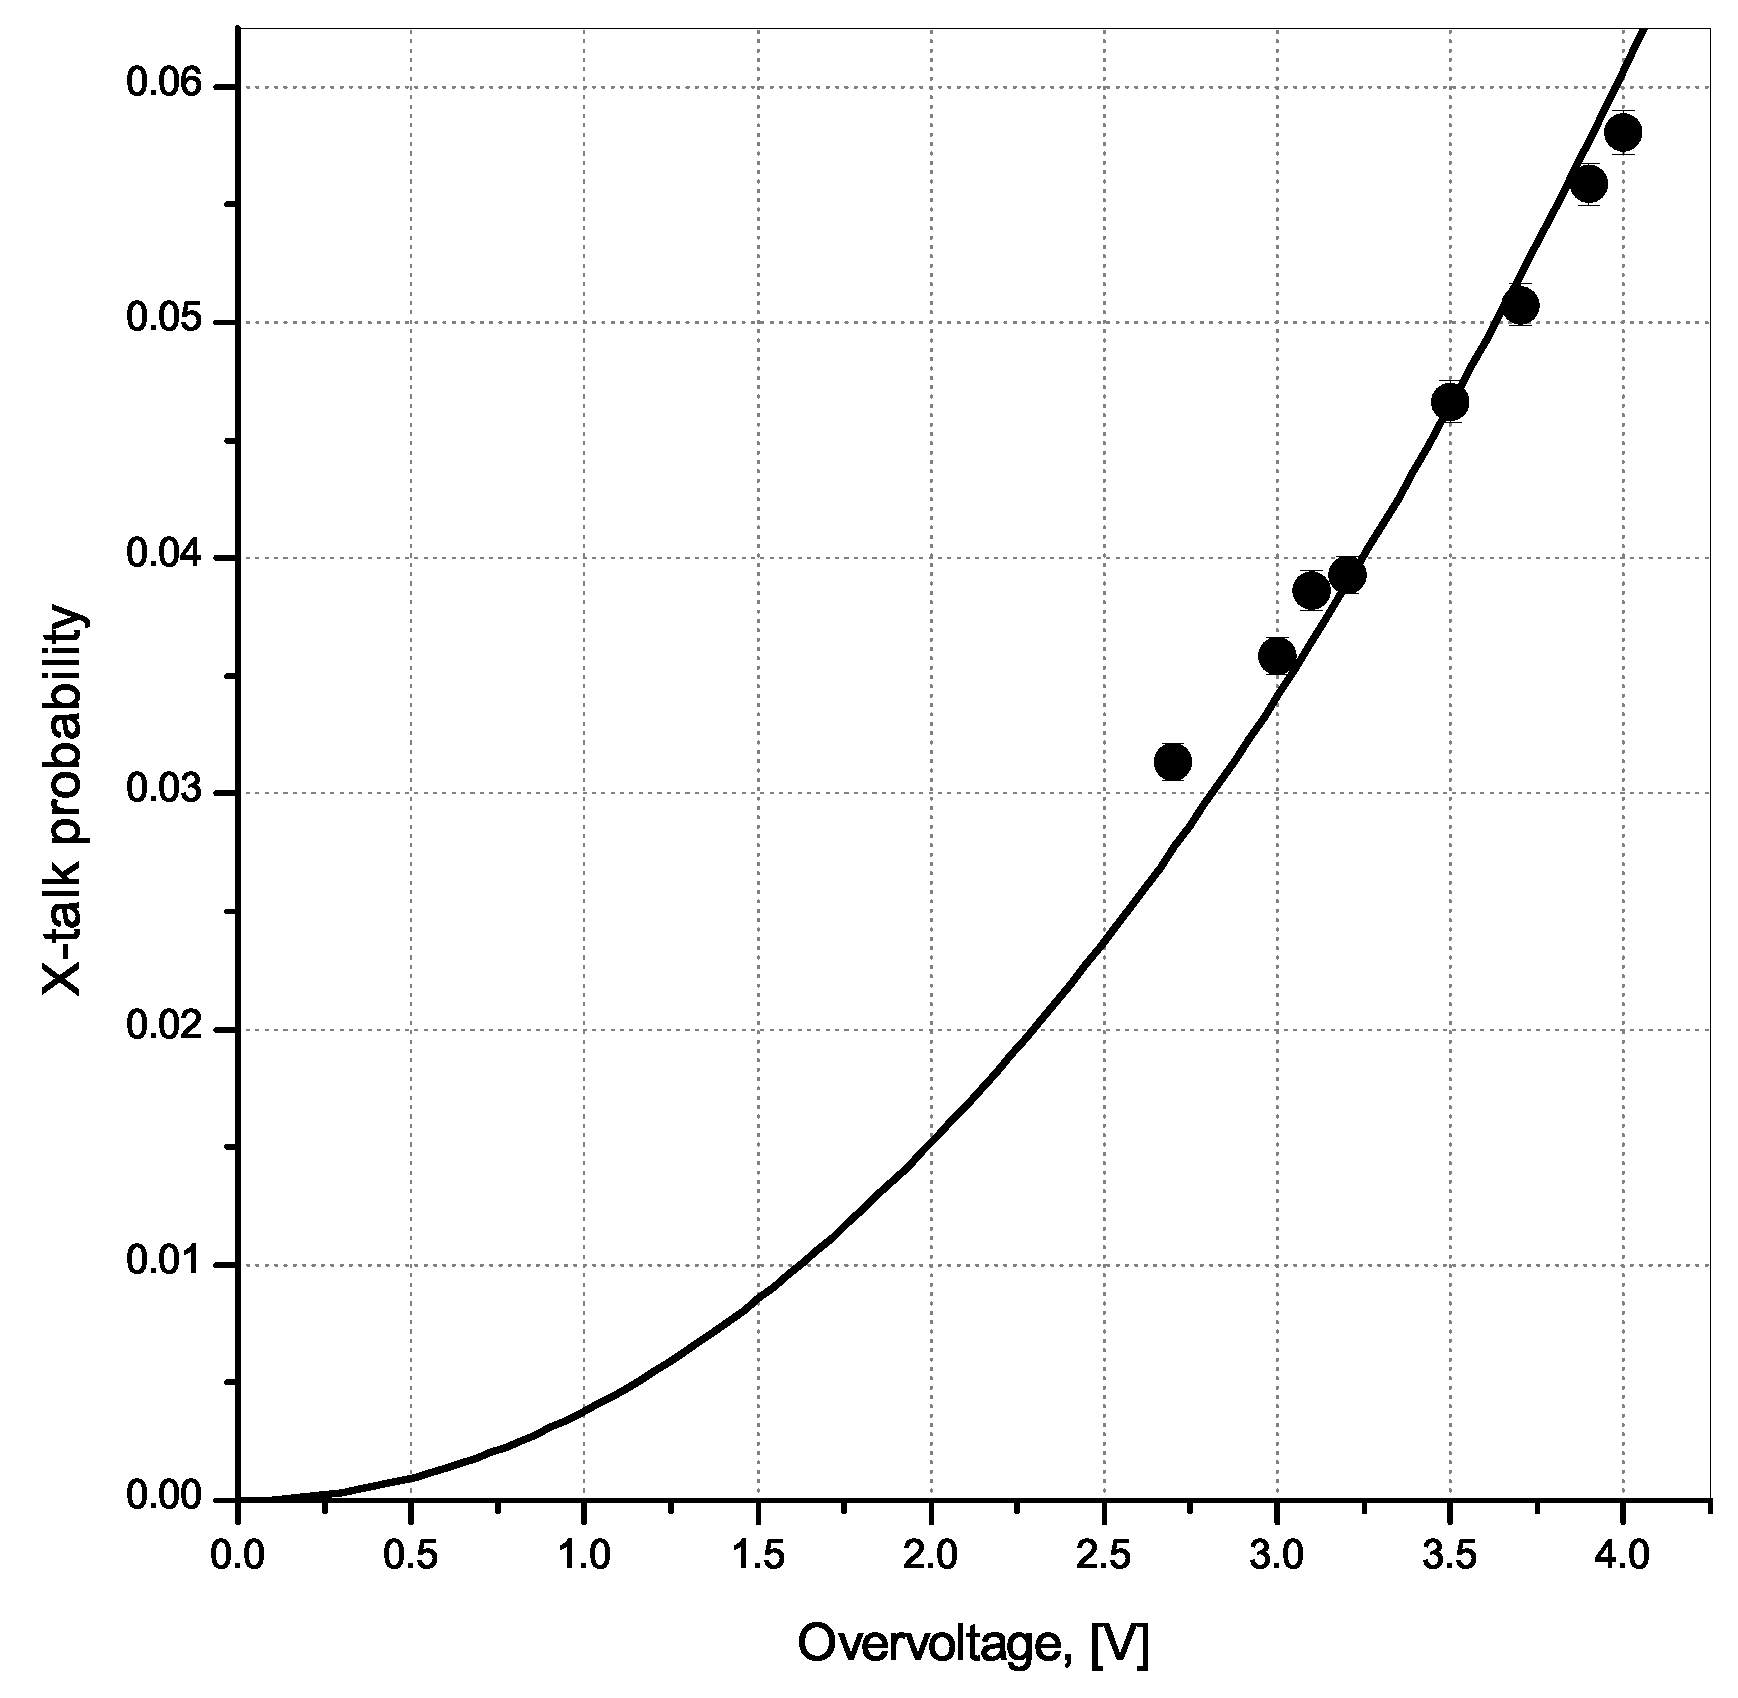
\includegraphics[width=0.47\textwidth]{KETEK_PM1125NS_SB0_x-tlak_vs_V_eng}
\\
\parbox[t]{0.47\textwidth}{\caption{The dependence of the cross-talk probability on an overvoltage at a fixed temperature for
Hamamatsu S13360-3050CS. The data were approximated by a quadratic function.}
\label{image:Hamamatsu_S13360-3050CS_xtalk_vs_V_rus}}
\hfill
\parbox[t]{0.47\textwidth}{\caption{The dependence of the cross-talk probability on an overvoltage at a fixed temperature for
KETEK PM1125NS-SB0. The data were approximated by a quadratic function.}
\label{image:KETEK_PM1125NS_SB0_x-tlak_vs_V_rus}}
\end{figure}

Based on the experimental data, it can be concluded that the cross-talk probability is temperature independent.

\subsection{Checking the model of four nearest neighbors}
It noted the existence of SiPM, which do not correspond to the model of four nearest neighbors \cite{Modeling crosstalk in silicon photomultipliers}.
In the model of four nearest neighbors it is assumed that a trigged cell can cause the triggering of only four nearest cells.
In this case, the cross-talk probability in the next cell $p$ is related to the full cross-talk probability $P_{x-talk}$ by the following equation
\begin{eqnarray}\label{eq:p vs xtalk}
(1 - p)^4 = 1 - P_{X-talk}
\end{eqnarray}

The full cross-talk probability was calculated by the Eq.(\ref{eq:xtalk_general}).
Then the $p$ value was calculated by Eq.(\ref{eq:p vs xtalk}).
It was calculated the theoretical probability that due to cross-talk only one cell triggered \cite{Modeling crosstalk in silicon photomultipliers}: $p_{2 phe}^{theory} = 4 \cdot p \cdot (1 - p)^6$.
On the other hand it was calculated the experimental probability $p_{2 phe}^{exp}$ as the ratio of events number $N_{2 p.e.}$ to the total number of events,
where $N_{2 p.e.} \approx  N_{B_{1}} / (N_{A_{1}} + N_{B_{1}} + N_{C_{1}})$.
As a result of measurements, it was found that the ratio $p_{2 phe}^{exp} / p_{2 phe}^{theory}$ for Hamamatsu S10362-11-100C varies from 1 to 1.08 depending on a temperature and an overvoltage, and for Hamamatsu S13360-3050CS and KETEK PM1125NS-SB0 this ratio varies from 0.98 to 1.02.
Thus it can be concluded that the model of four nearest neighbors works well for considered SiPMs.

\subsection{After-pulses}

As a result of spectrum approximation we fond also probabilities and time constants for after-pulses.
The obtained data are shown in Fig.~\ref{image:Hamamatsu_S10362-11-100C_p_f_vs_T}, \ref{image:Hamamatsu_S10362-11-100C_p_f_vs_V}, \ref{image:Hamamatsu_S10362-11-100C_p_s_vs_T}, \ref{image:Hamamatsu_S10362-11-100C_p_s_vs_V}, \ref{image:Hamamatsu_S10362-11-100C_tau_f_vs_T}, \ref{image:Hamamatsu_S10362-11-100C_tau_f_vs_V}, \ref{image:Hamamatsu_S10362-11-100C_tau_s_vs_T},
 \ref{image:Hamamatsu_S10362-11-100C_tau_s_vs_V}, \ref{image:Hamamatsu_S13360-3050CS_p_f_vs_V_rus}, \ref{image:Hamamatsu_S13360-3050CS_tau_s_vs_V}, \ref{image:KETEK_PM1125NS_SB0_p_f_vs_V_rus}, \ref{image:KETEK_PM1125NS_SB0_tau_f_vs_V_rus}.

\begin{figure}[h]
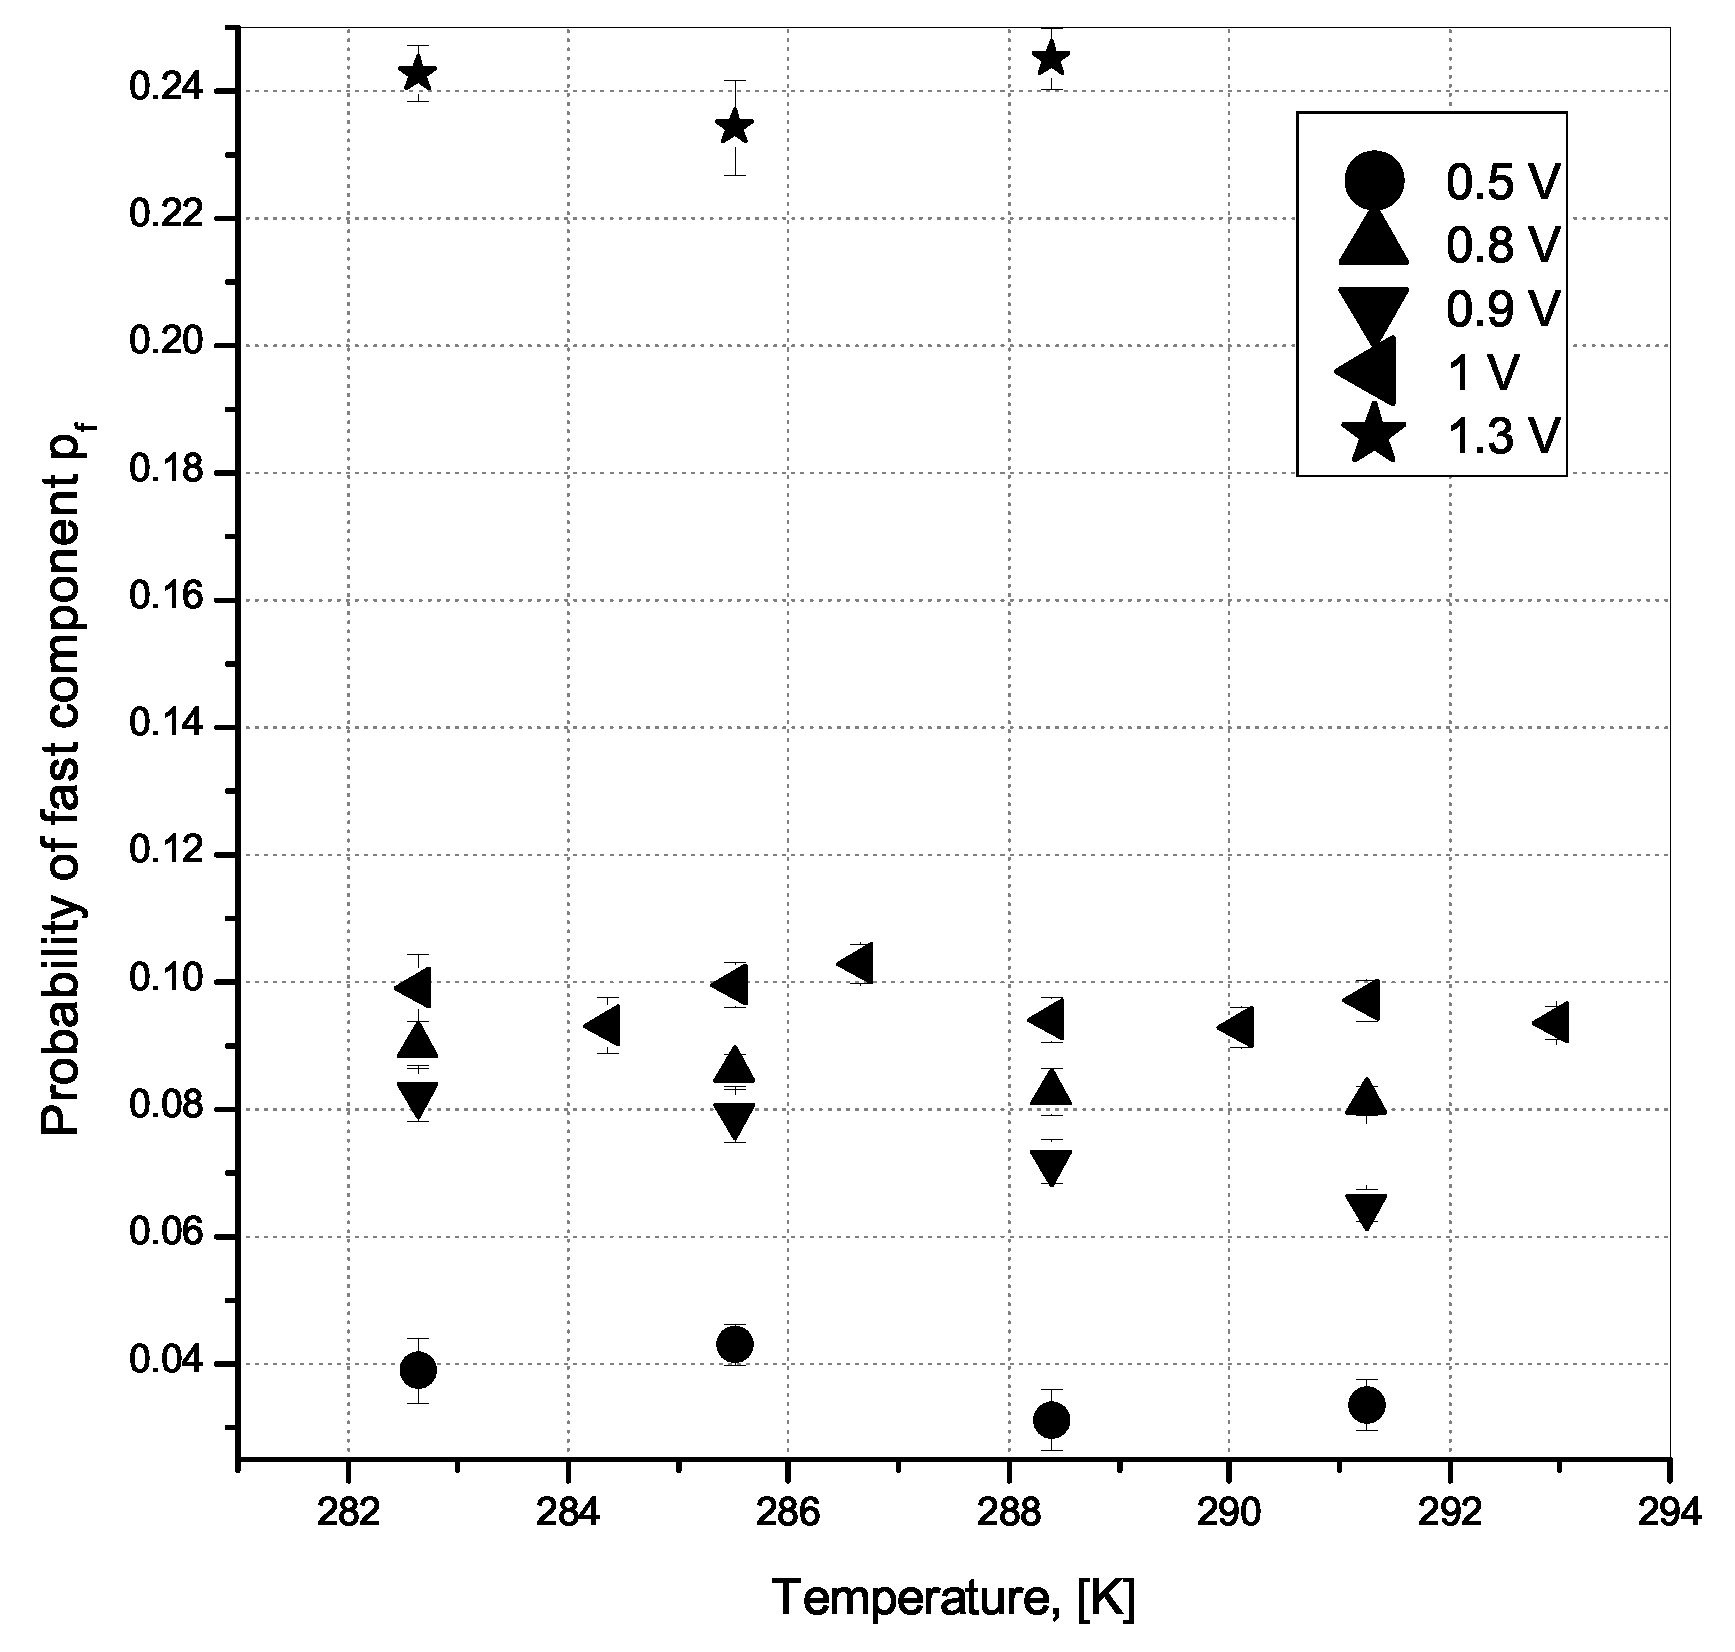
\includegraphics[width=0.47\textwidth]{Hamamatsu_S10362-11-100C_p_f_vs_T_eng}
\hfill
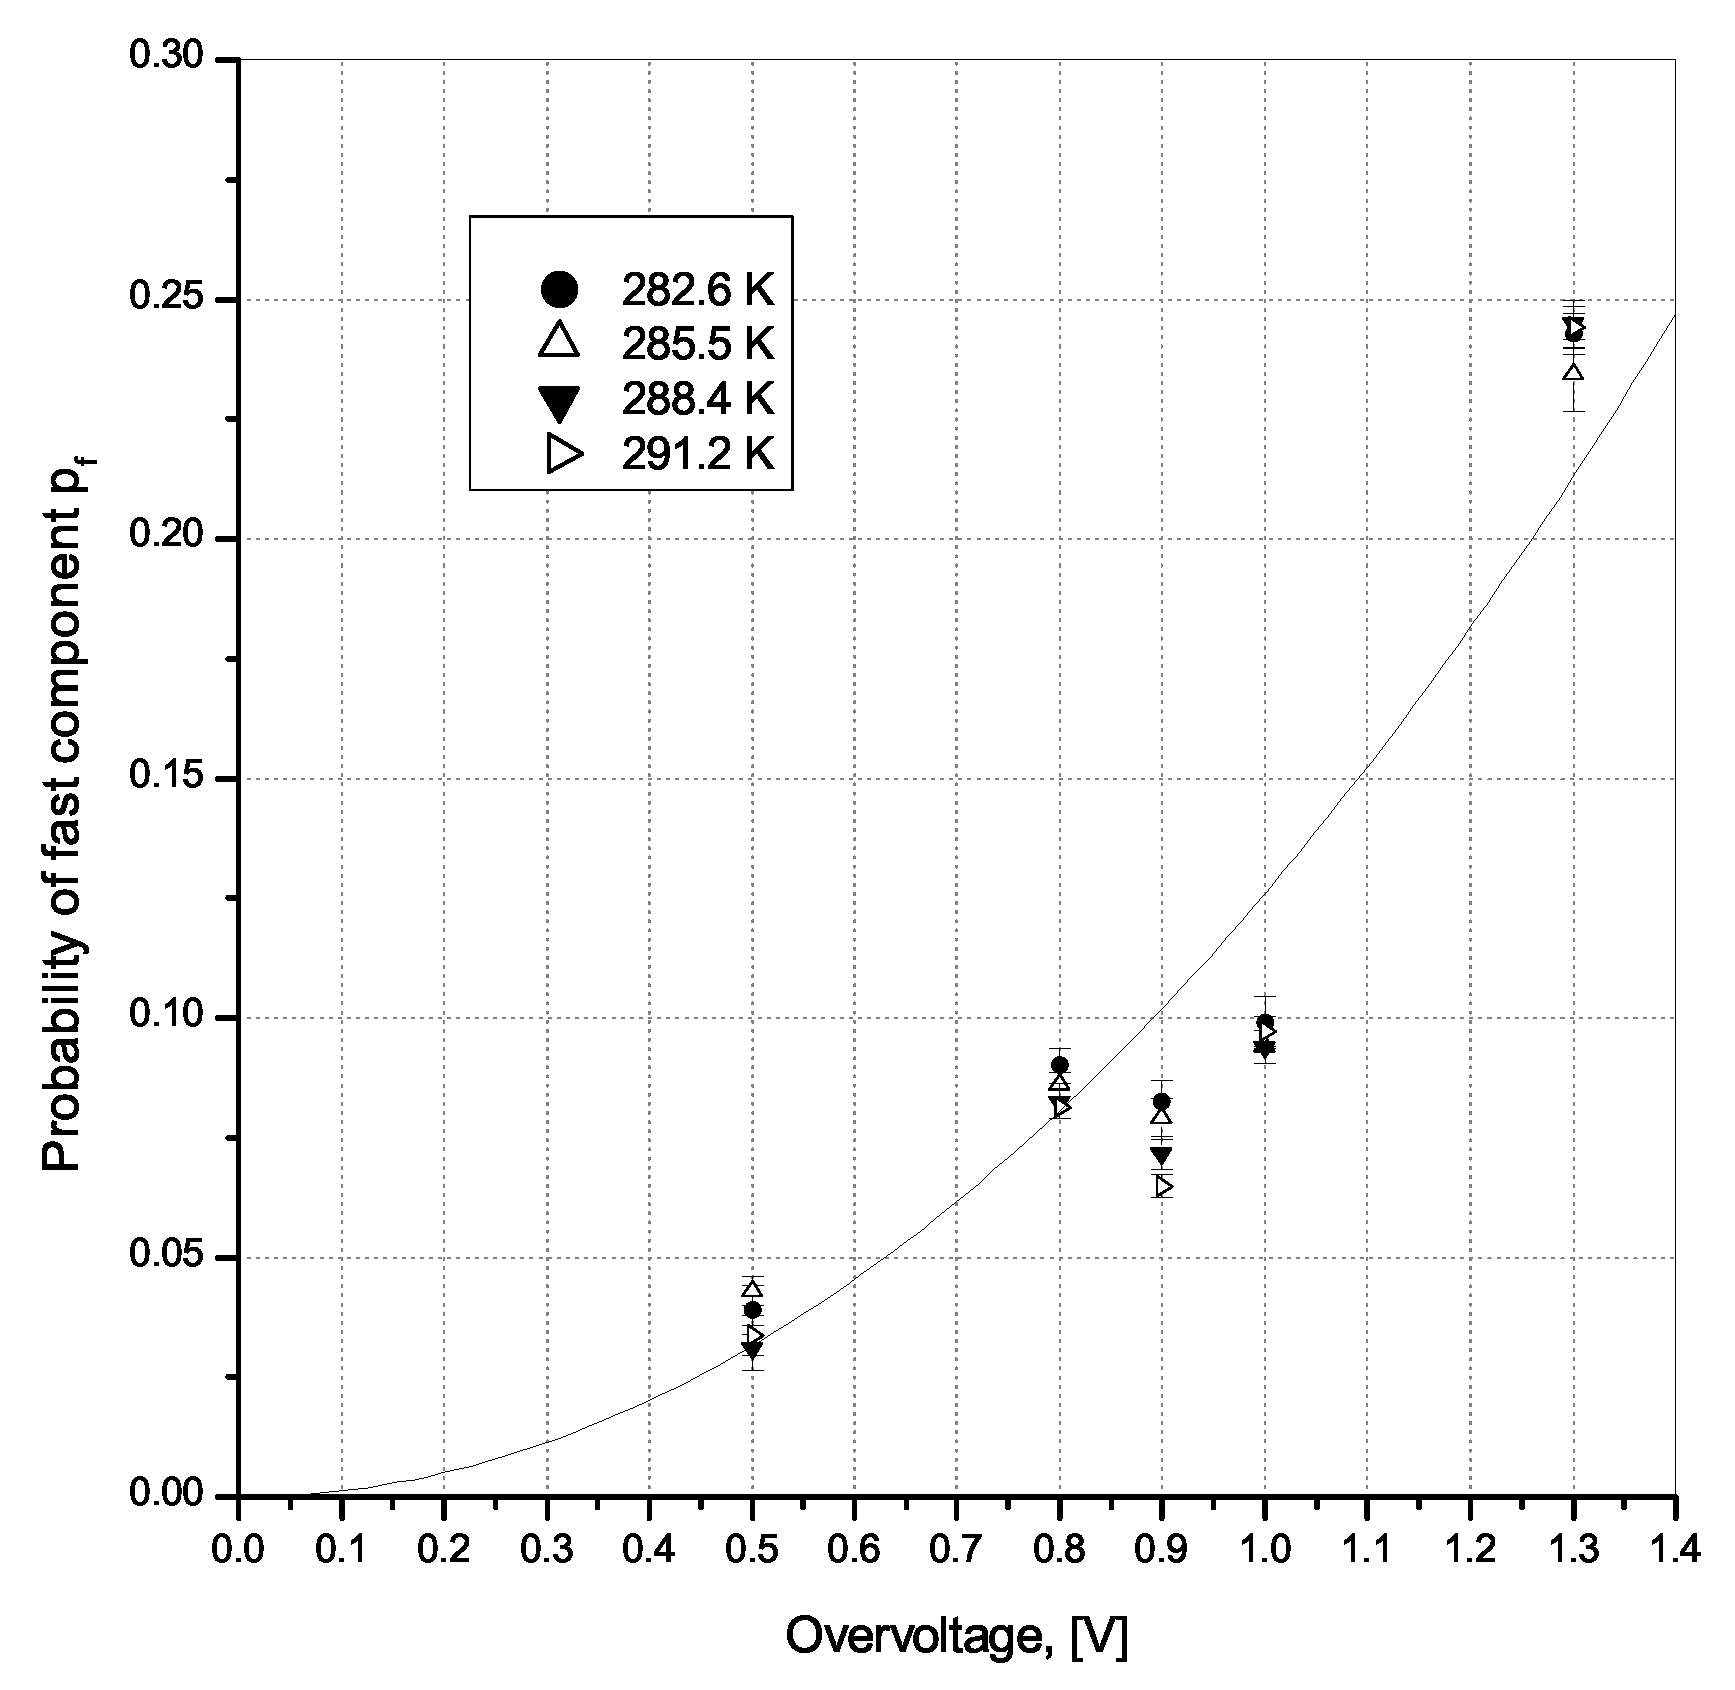
\includegraphics[width=0.47\textwidth]{Hamamatsu_S10362-11-100C_p_f_vs_V_eng}
\\
\parbox[t]{0.47\textwidth}{\caption{The dependence of the fast component probability $p_{f}$ for an after-pulse on a temperature at a fixed overvoltage for
Hamamatsu S10362-11-100C.}
\label{image:Hamamatsu_S10362-11-100C_p_f_vs_T}}
\hfill
\parbox[t]{0.47\textwidth}{\caption{The dependence of the fast component probability $p_{f}$ for an after-pulse on an overvoltage at a fixed temperature for
Hamamatsu S10362-11-100C. The data were approximated by a quadratic function.}
\label{image:Hamamatsu_S10362-11-100C_p_f_vs_V}}
\end{figure}

\begin{figure}[h]
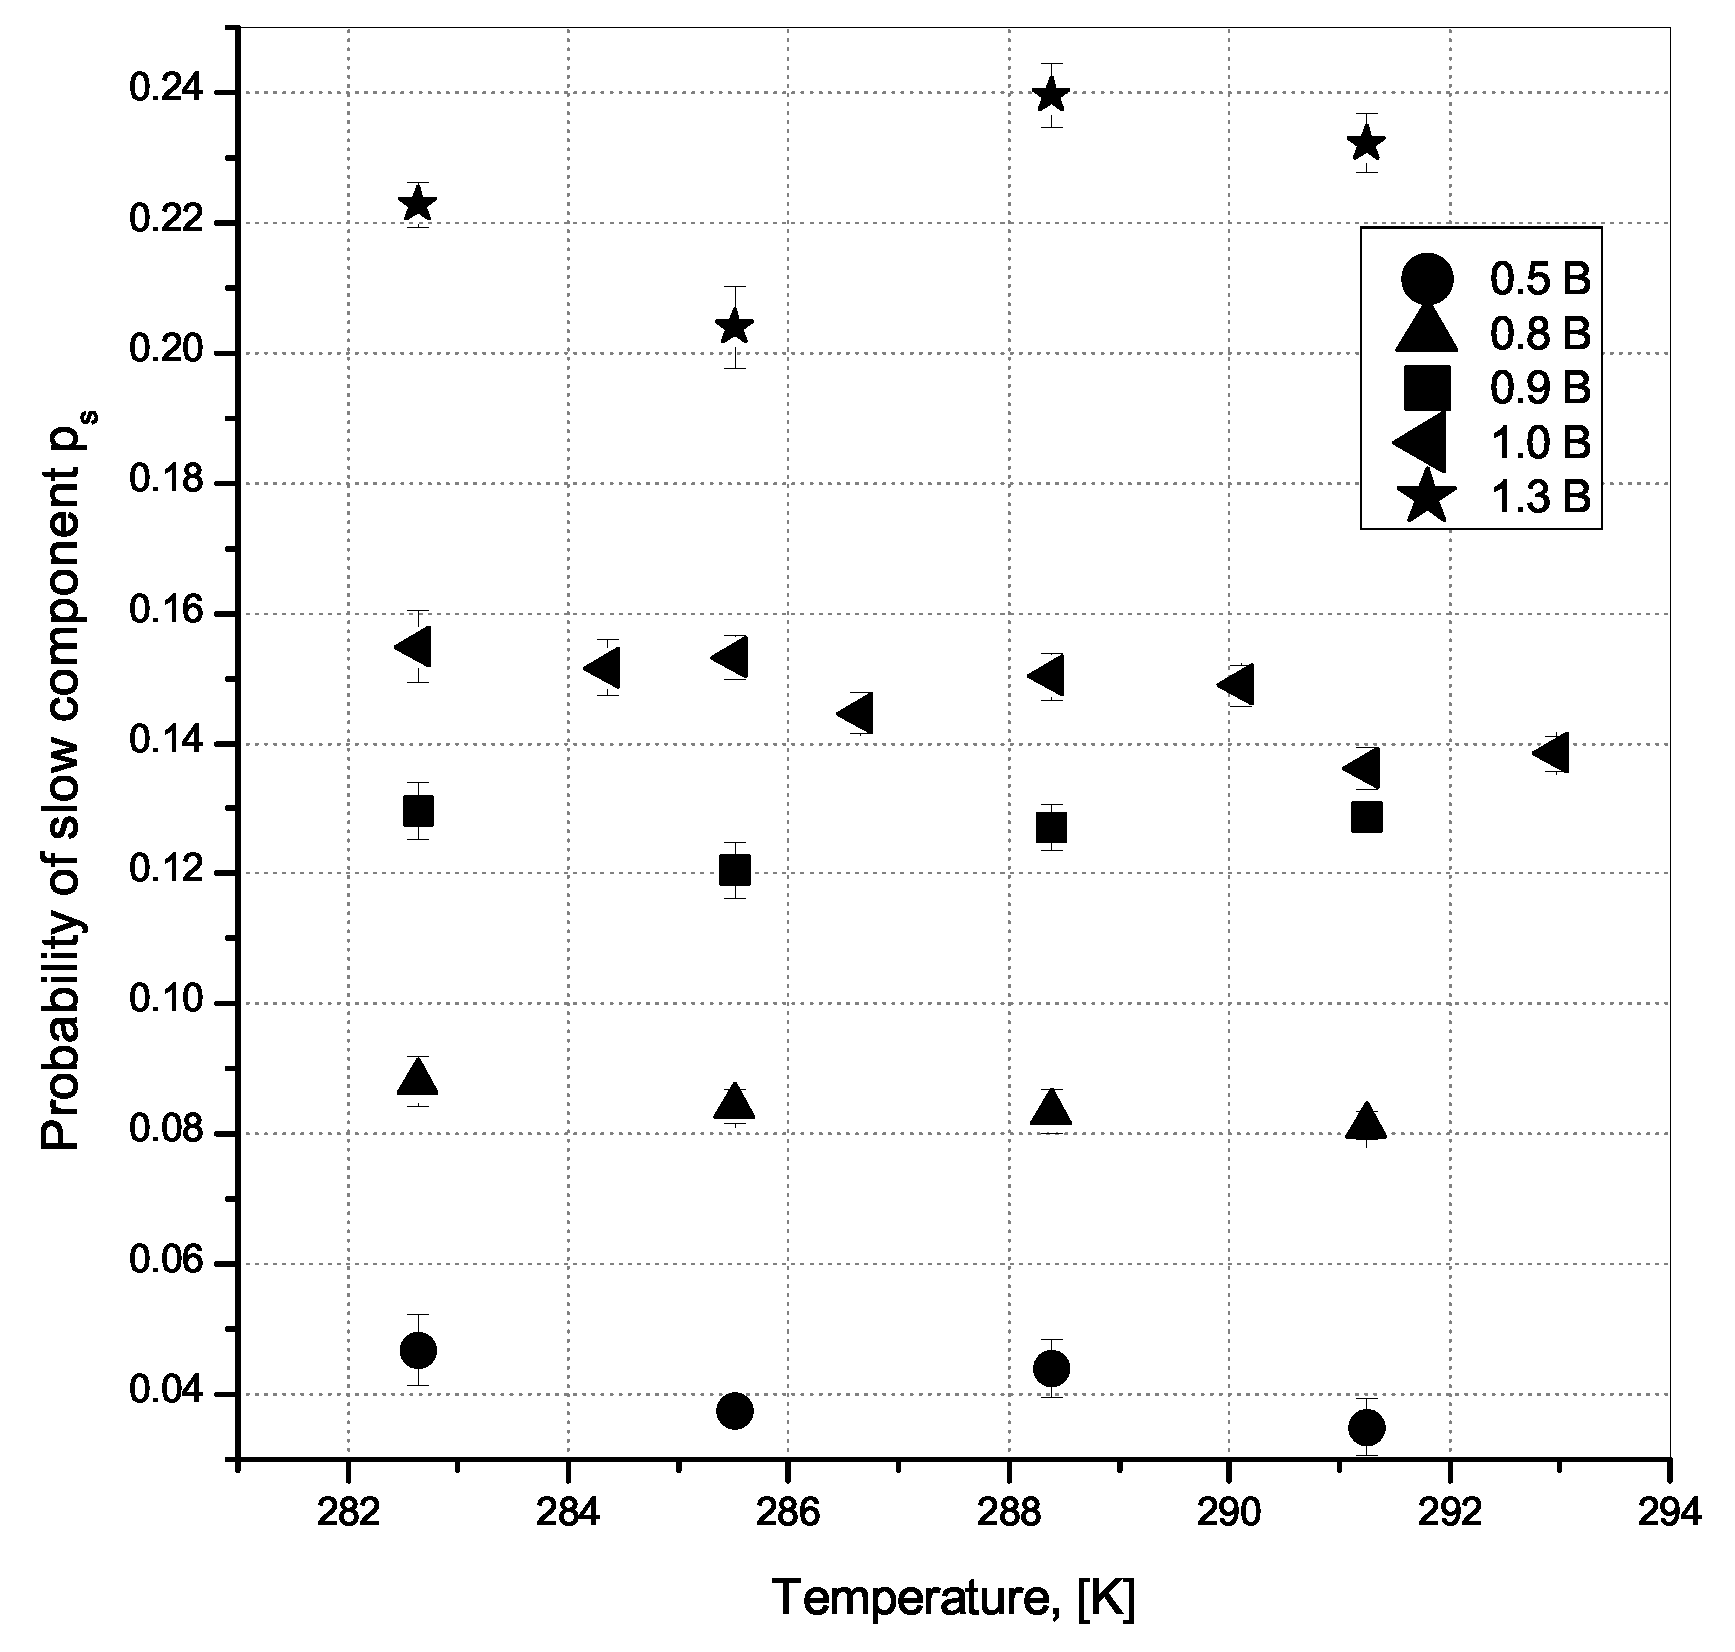
\includegraphics[width=0.47\textwidth]{Hamamatsu_S10362-11-100C_p_s_vs_T_eng}
\hfill
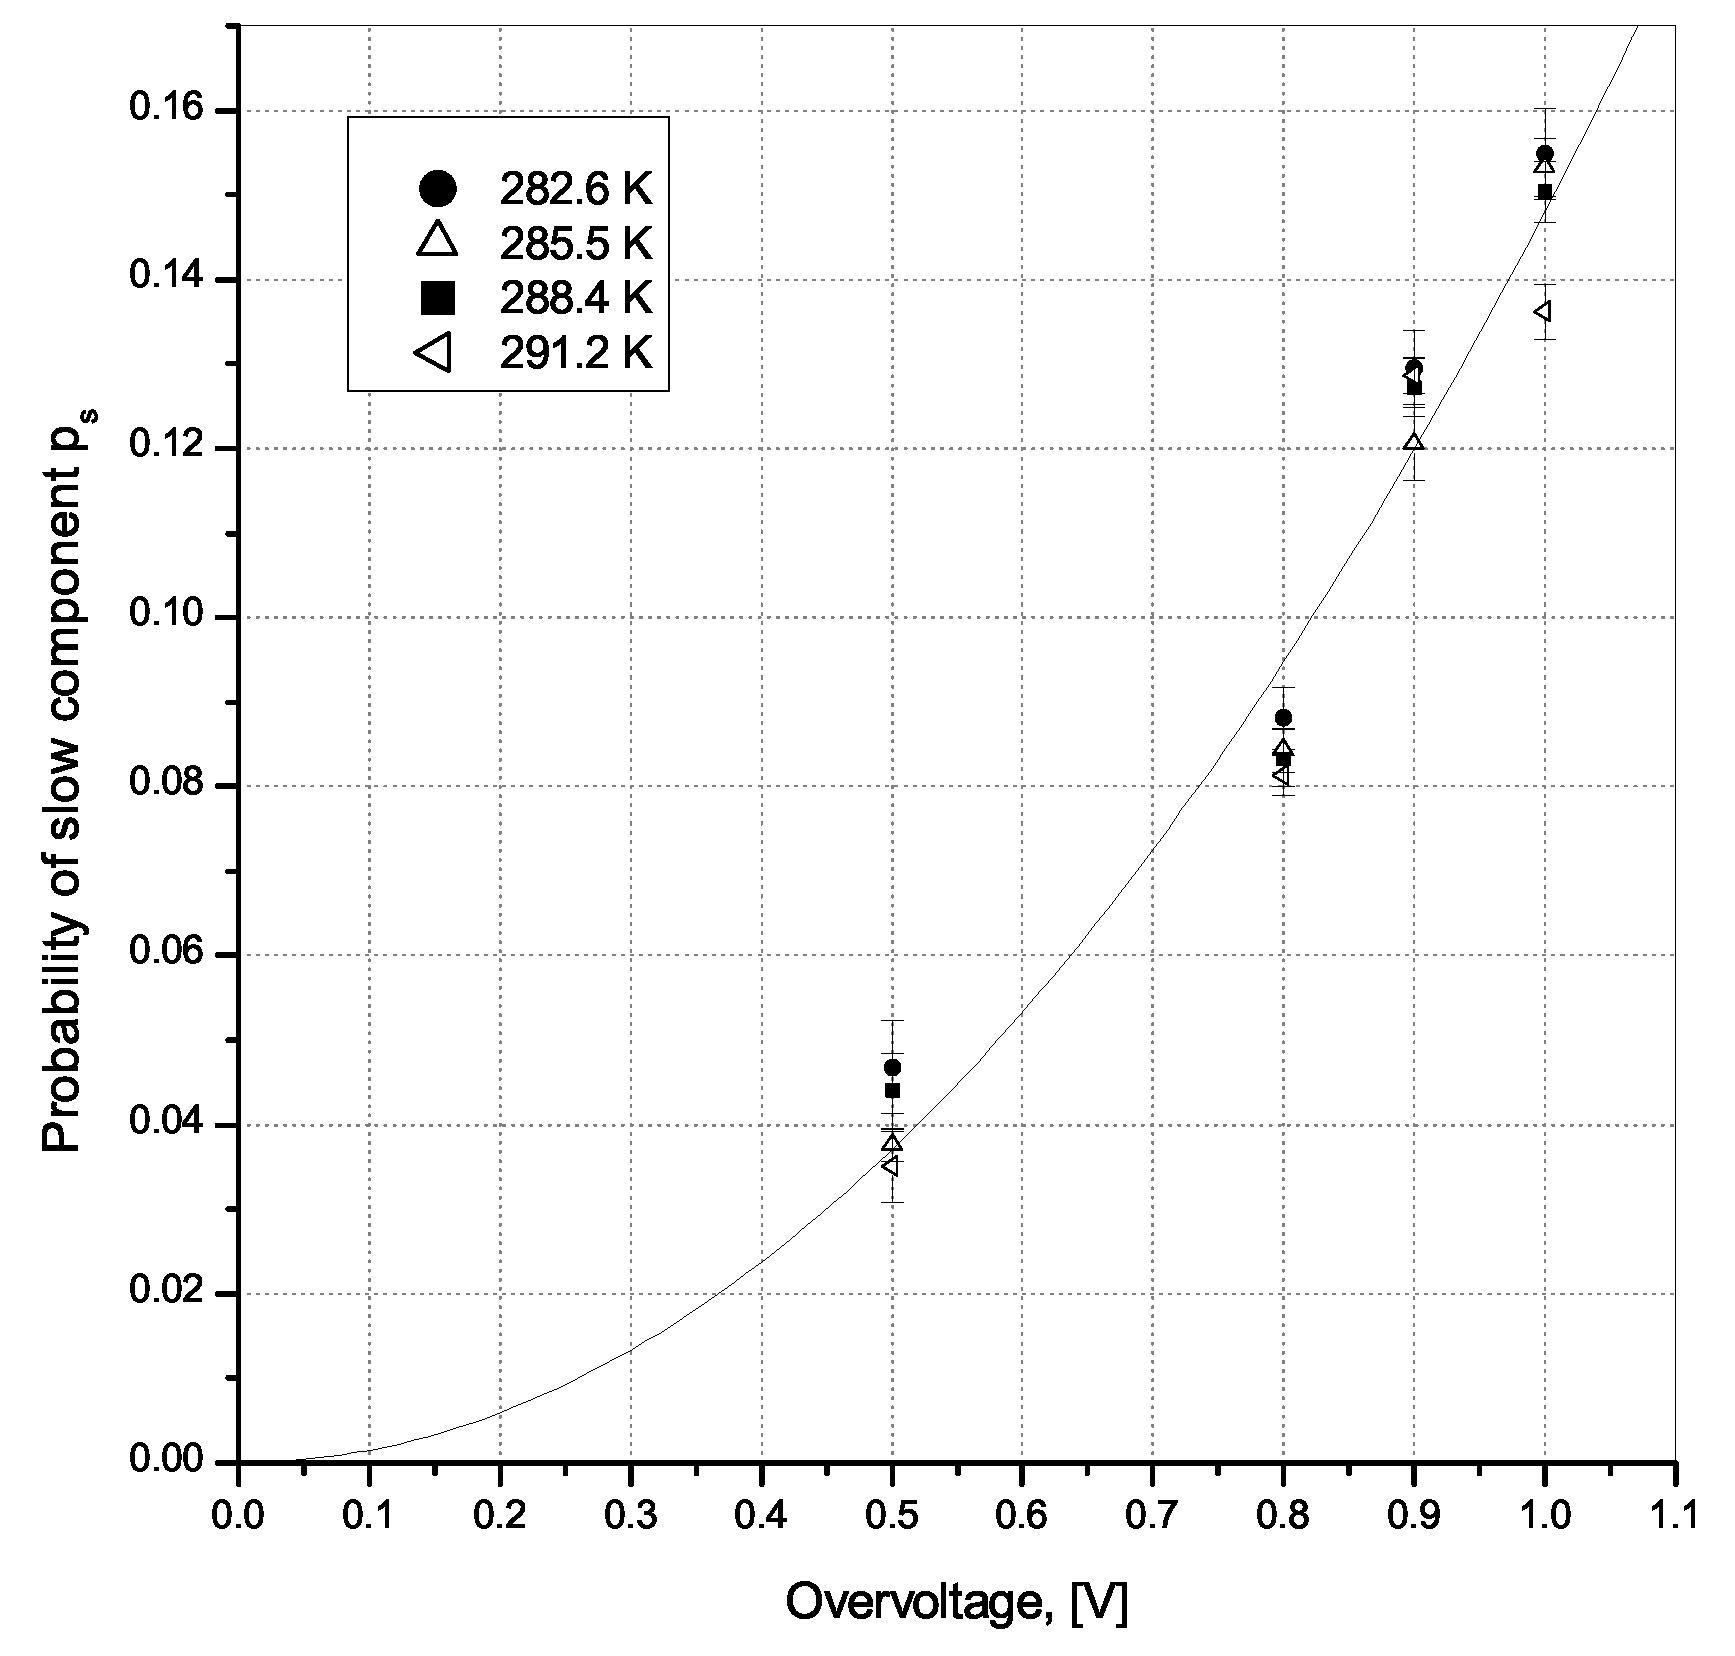
\includegraphics[width=0.47\textwidth]{Hamamatsu_S10362-11-100C_p_s_vs_V_eng}
\\
\parbox[t]{0.47\textwidth}{\caption{The dependence of the slow component probability $p_{s}$ for an after-pulse on a temperature at a fixed overvoltage for
Hamamatsu S10362-11-100C.}
\label{image:Hamamatsu_S10362-11-100C_p_s_vs_T}}
\hfill
\parbox[t]{0.47\textwidth}{\caption{The dependence of the slow component probability $p_{s}$ for an after-pulse on an overvoltage at a fixed temperature for
Hamamatsu S10362-11-100C. The data were approximated by a quadratic function.}
\label{image:Hamamatsu_S10362-11-100C_p_s_vs_V}}
\end{figure}

\begin{figure}[h]
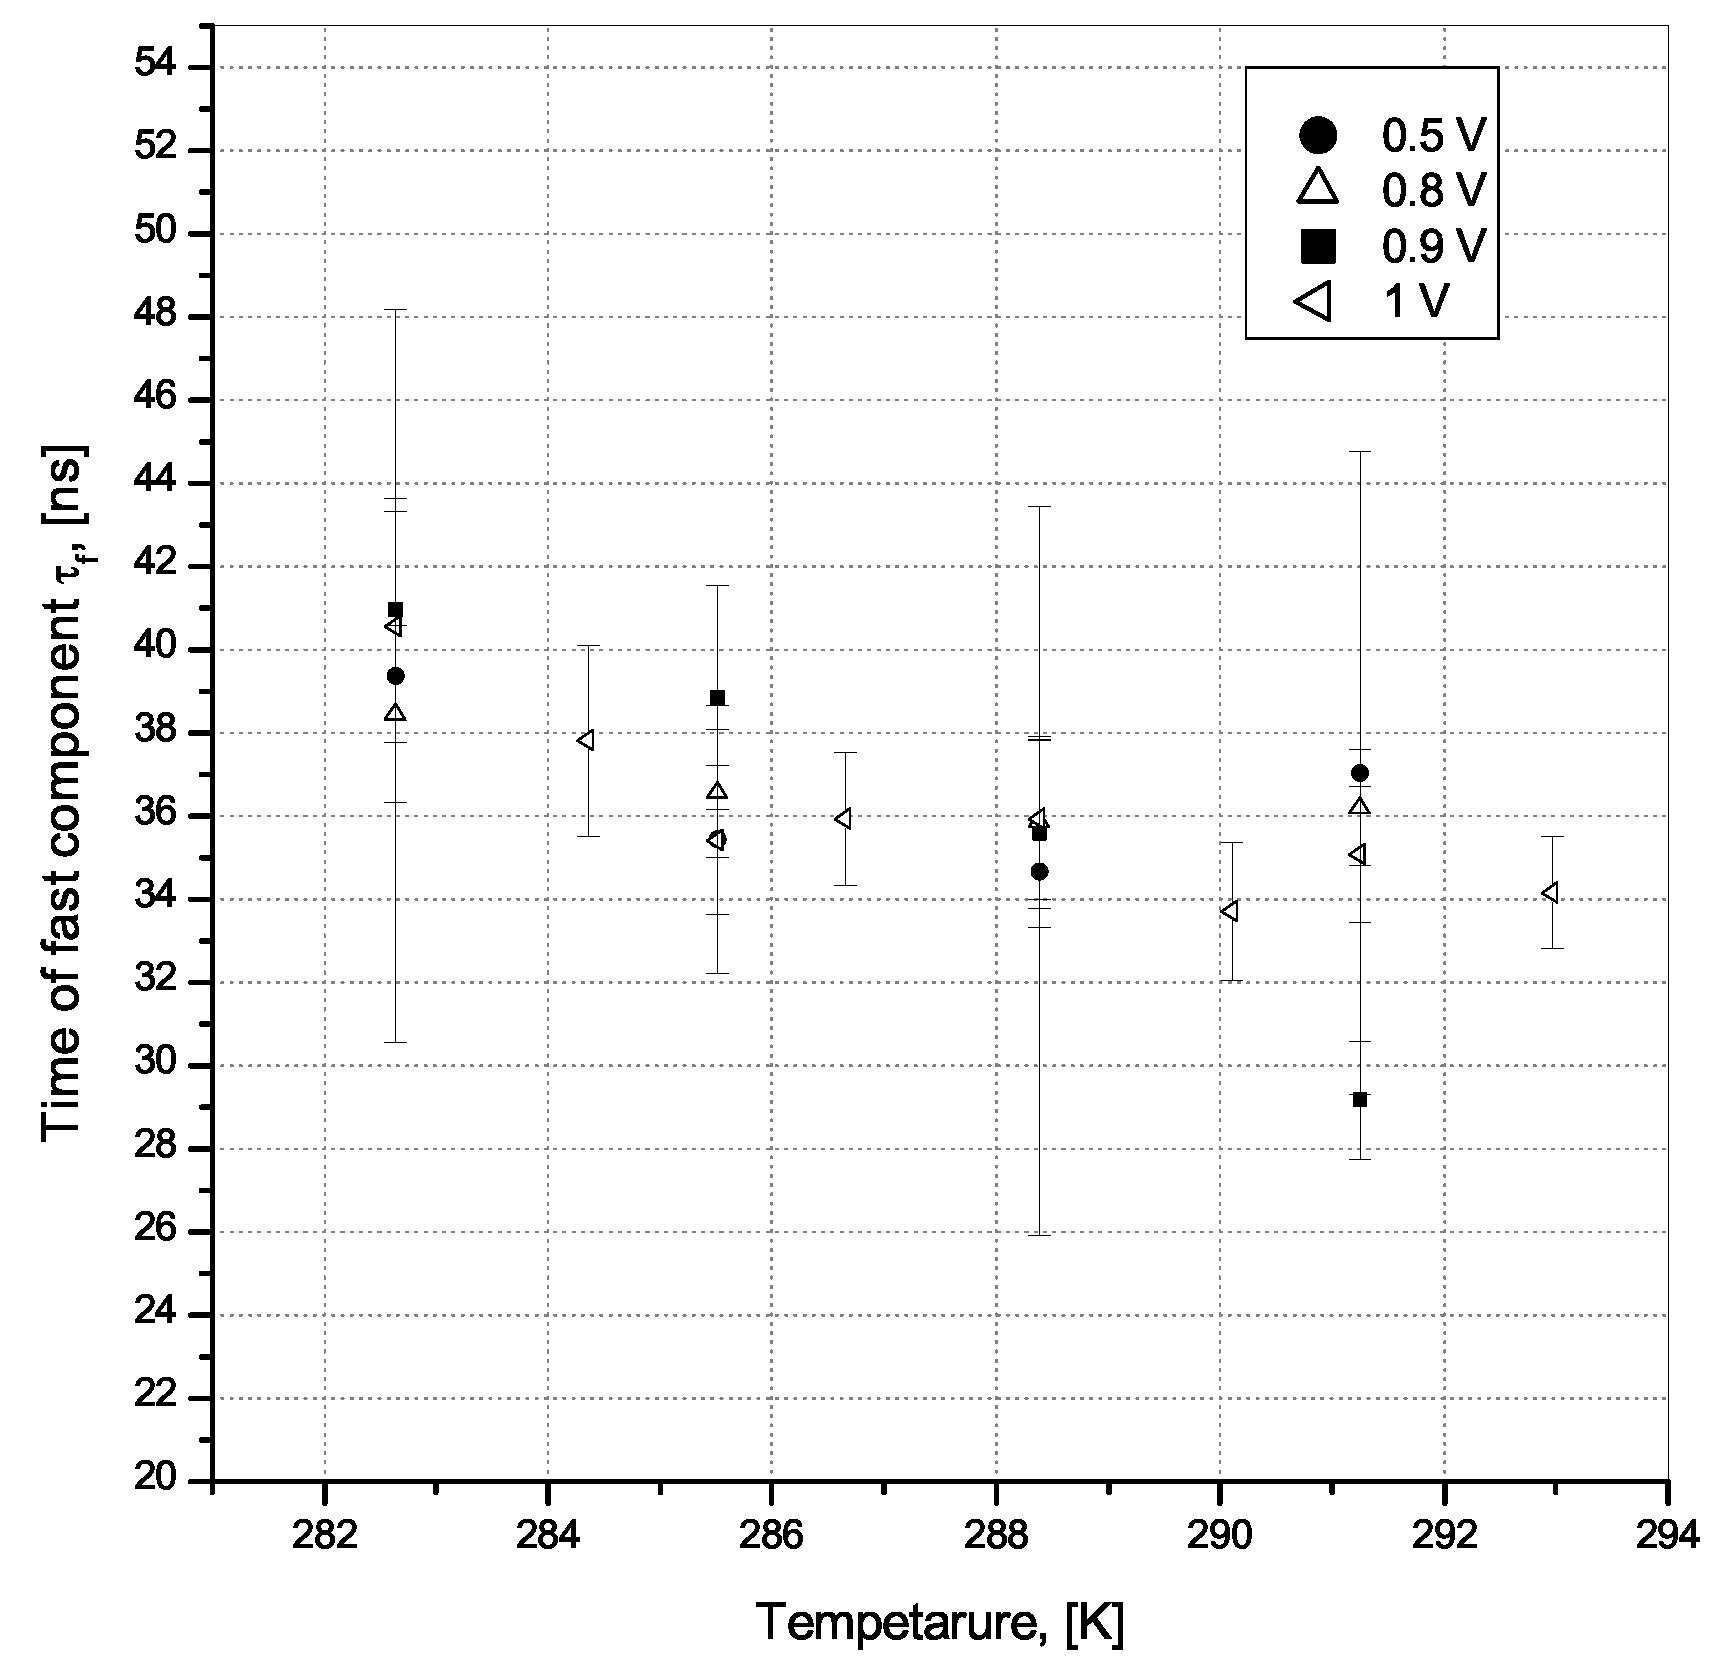
\includegraphics[width=0.47\textwidth]{Hamamatsu_S10362-11-100C_tau_f_vs_T_eng}
\hfill
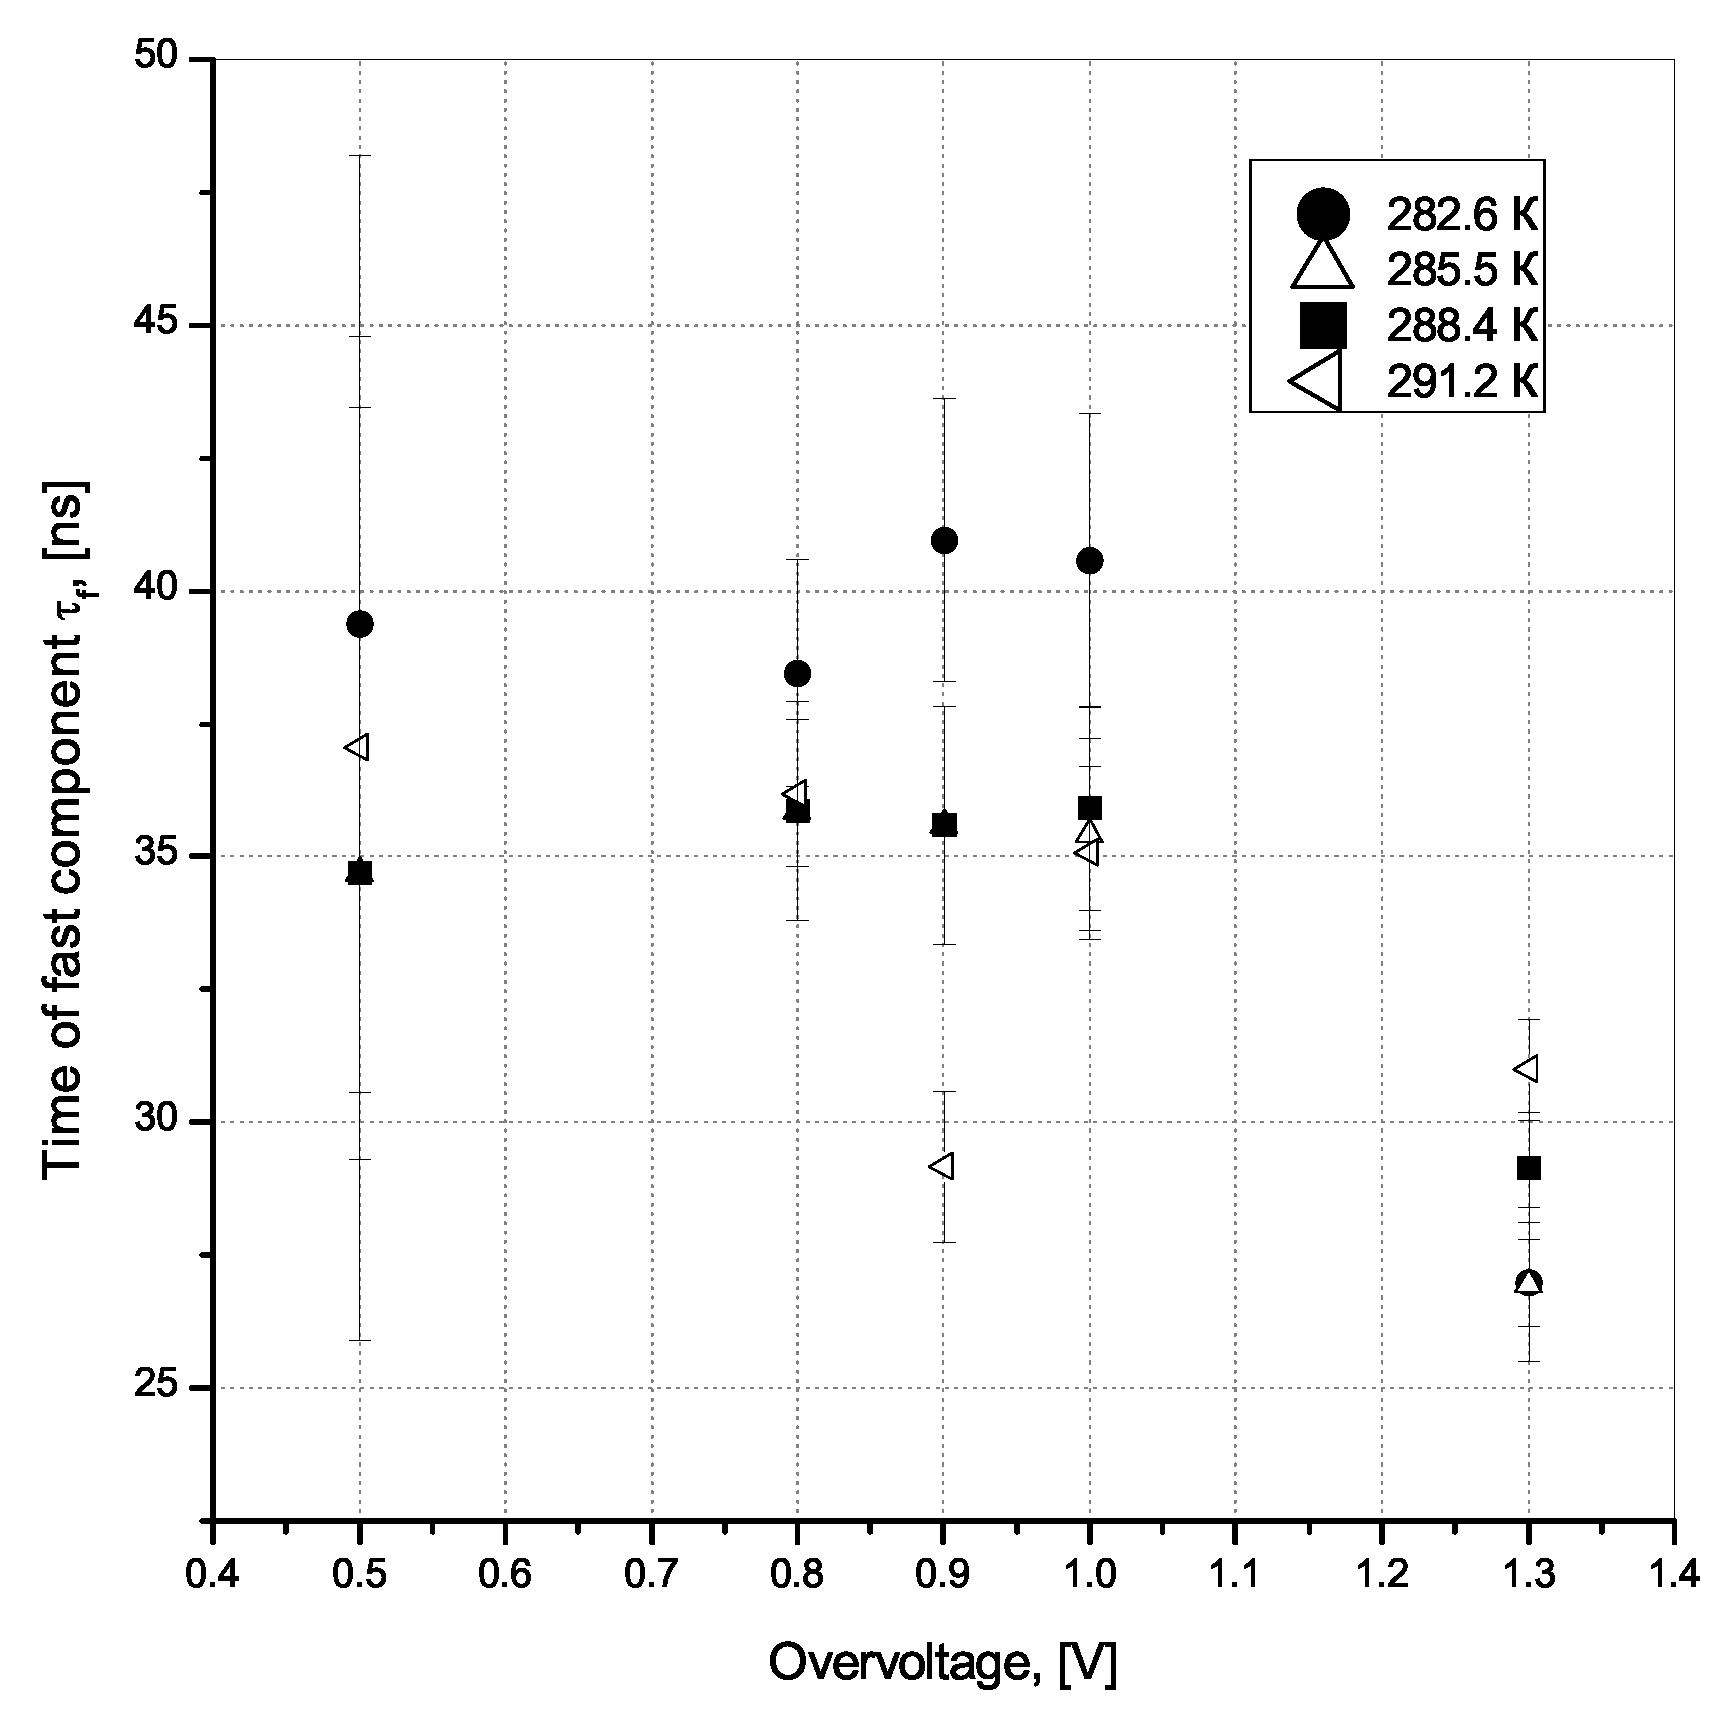
\includegraphics[width=0.47\textwidth]{Hamamatsu_S10362-11-100C_tau_f_vs_V_eng}
\\
\parbox[t]{0.47\textwidth}{\caption{The dependence of the fast time constant $\tau_{f}$ for an after-pulse on a temperature at a fixed overvoltage for
Hamamatsu S10362-11-100C.}
\label{image:Hamamatsu_S10362-11-100C_tau_f_vs_T}}
\hfill
\parbox[t]{0.47\textwidth}{\caption{The dependence of the fast time constant $\tau_{f}$ for an after-pulse on an overvoltage at a fixed temperature for
Hamamatsu S10362-11-100C.}
\label{image:Hamamatsu_S10362-11-100C_tau_f_vs_V}}
\end{figure}

%\if 0
\begin{figure}[h]
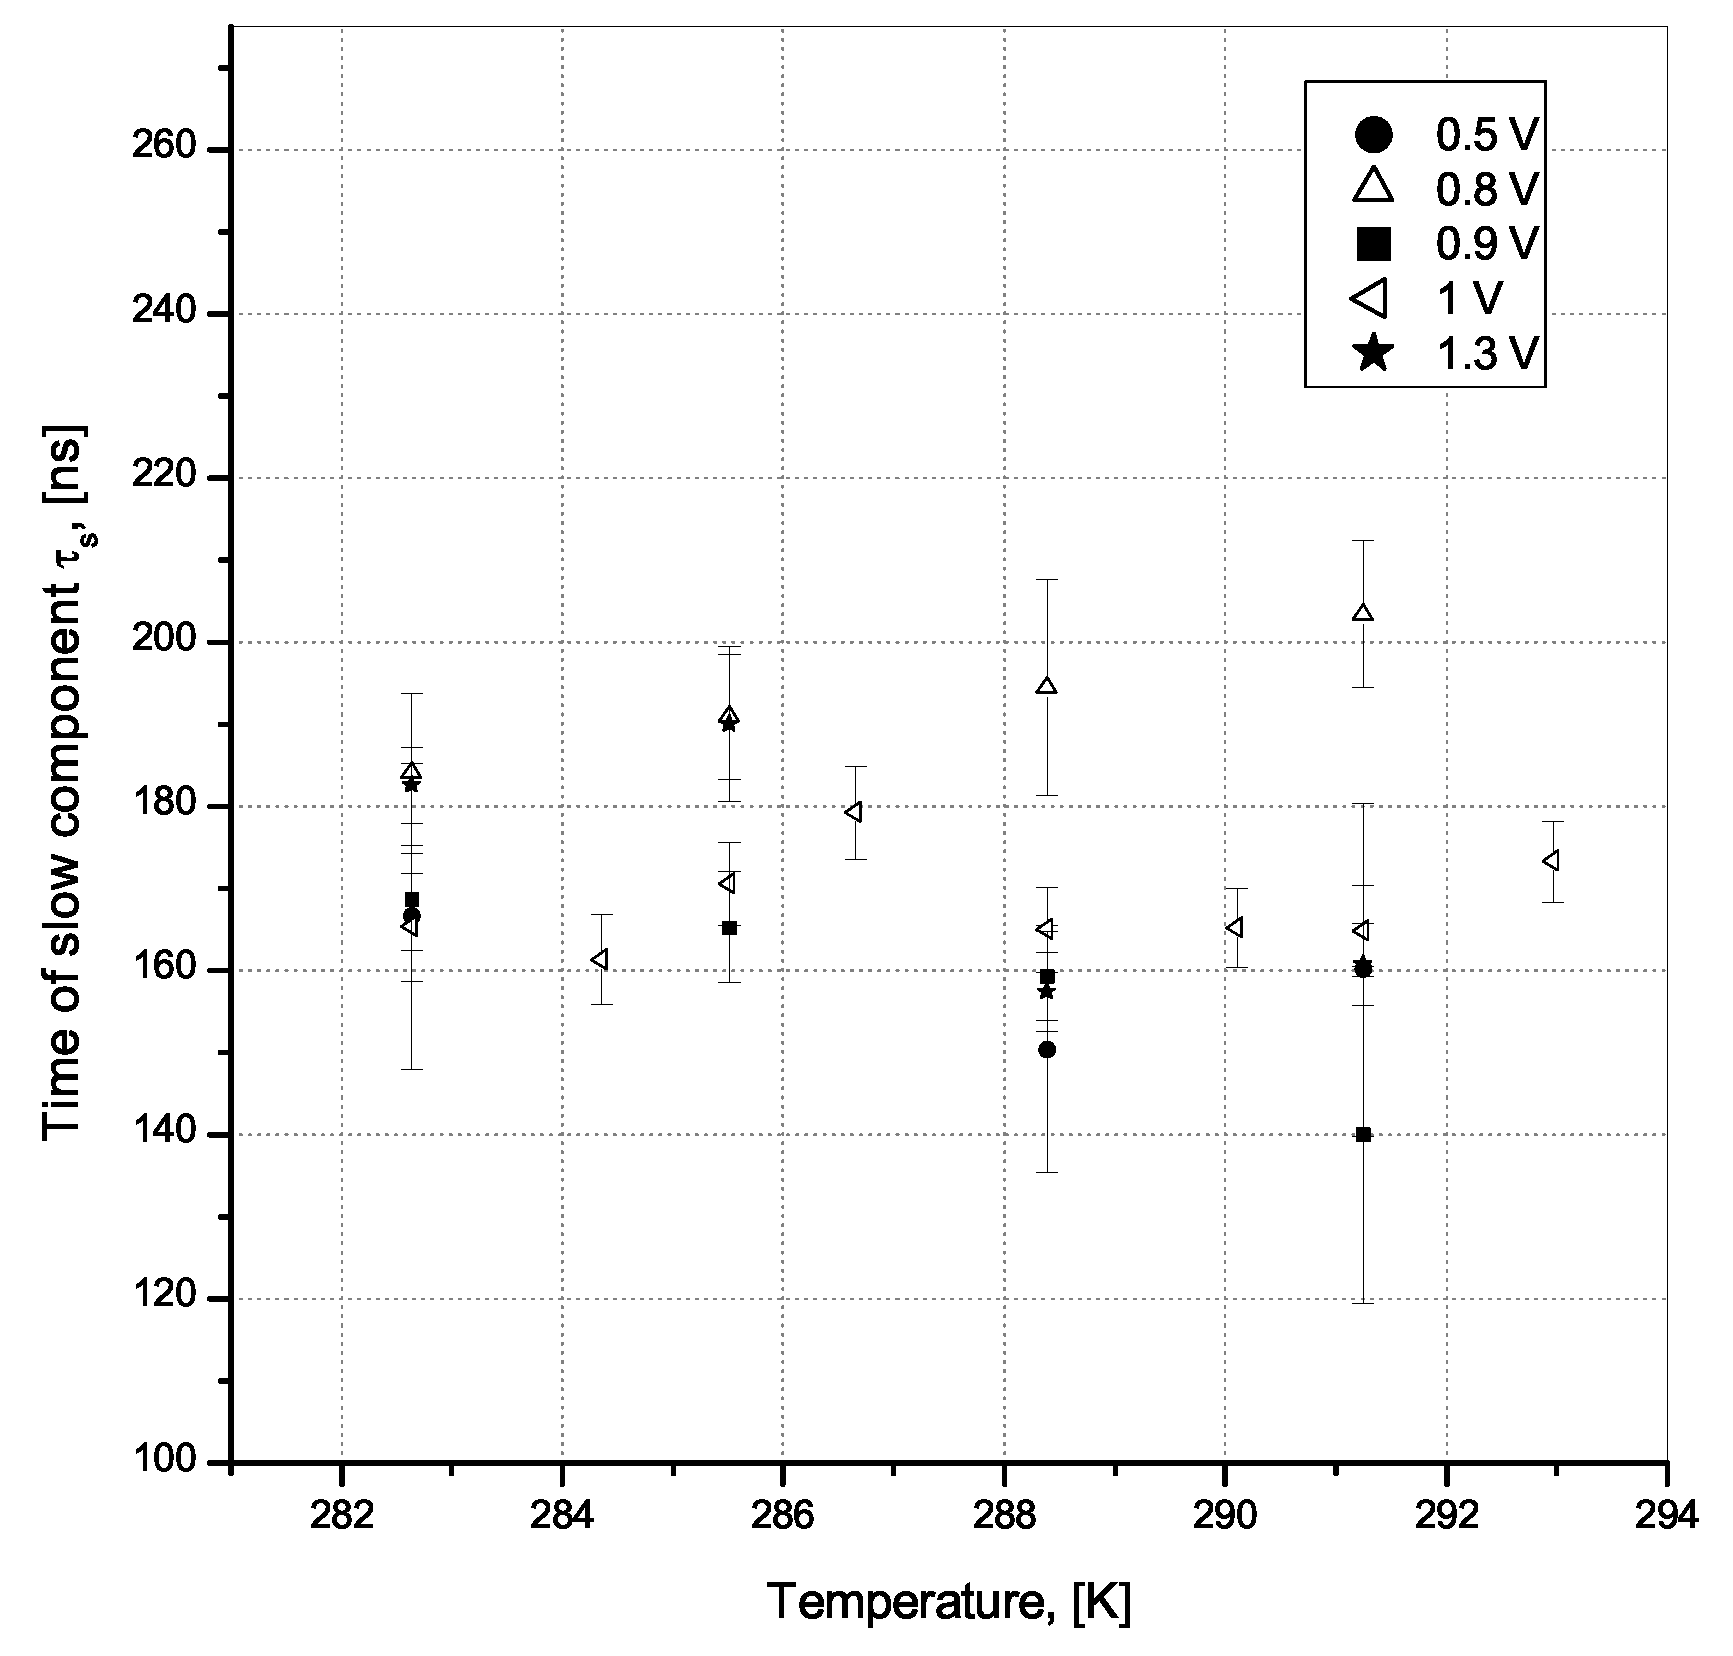
\includegraphics[width=0.47\textwidth]{Hamamatsu_S10362-11-100C_tau_s_vs_T_eng}
\hfill
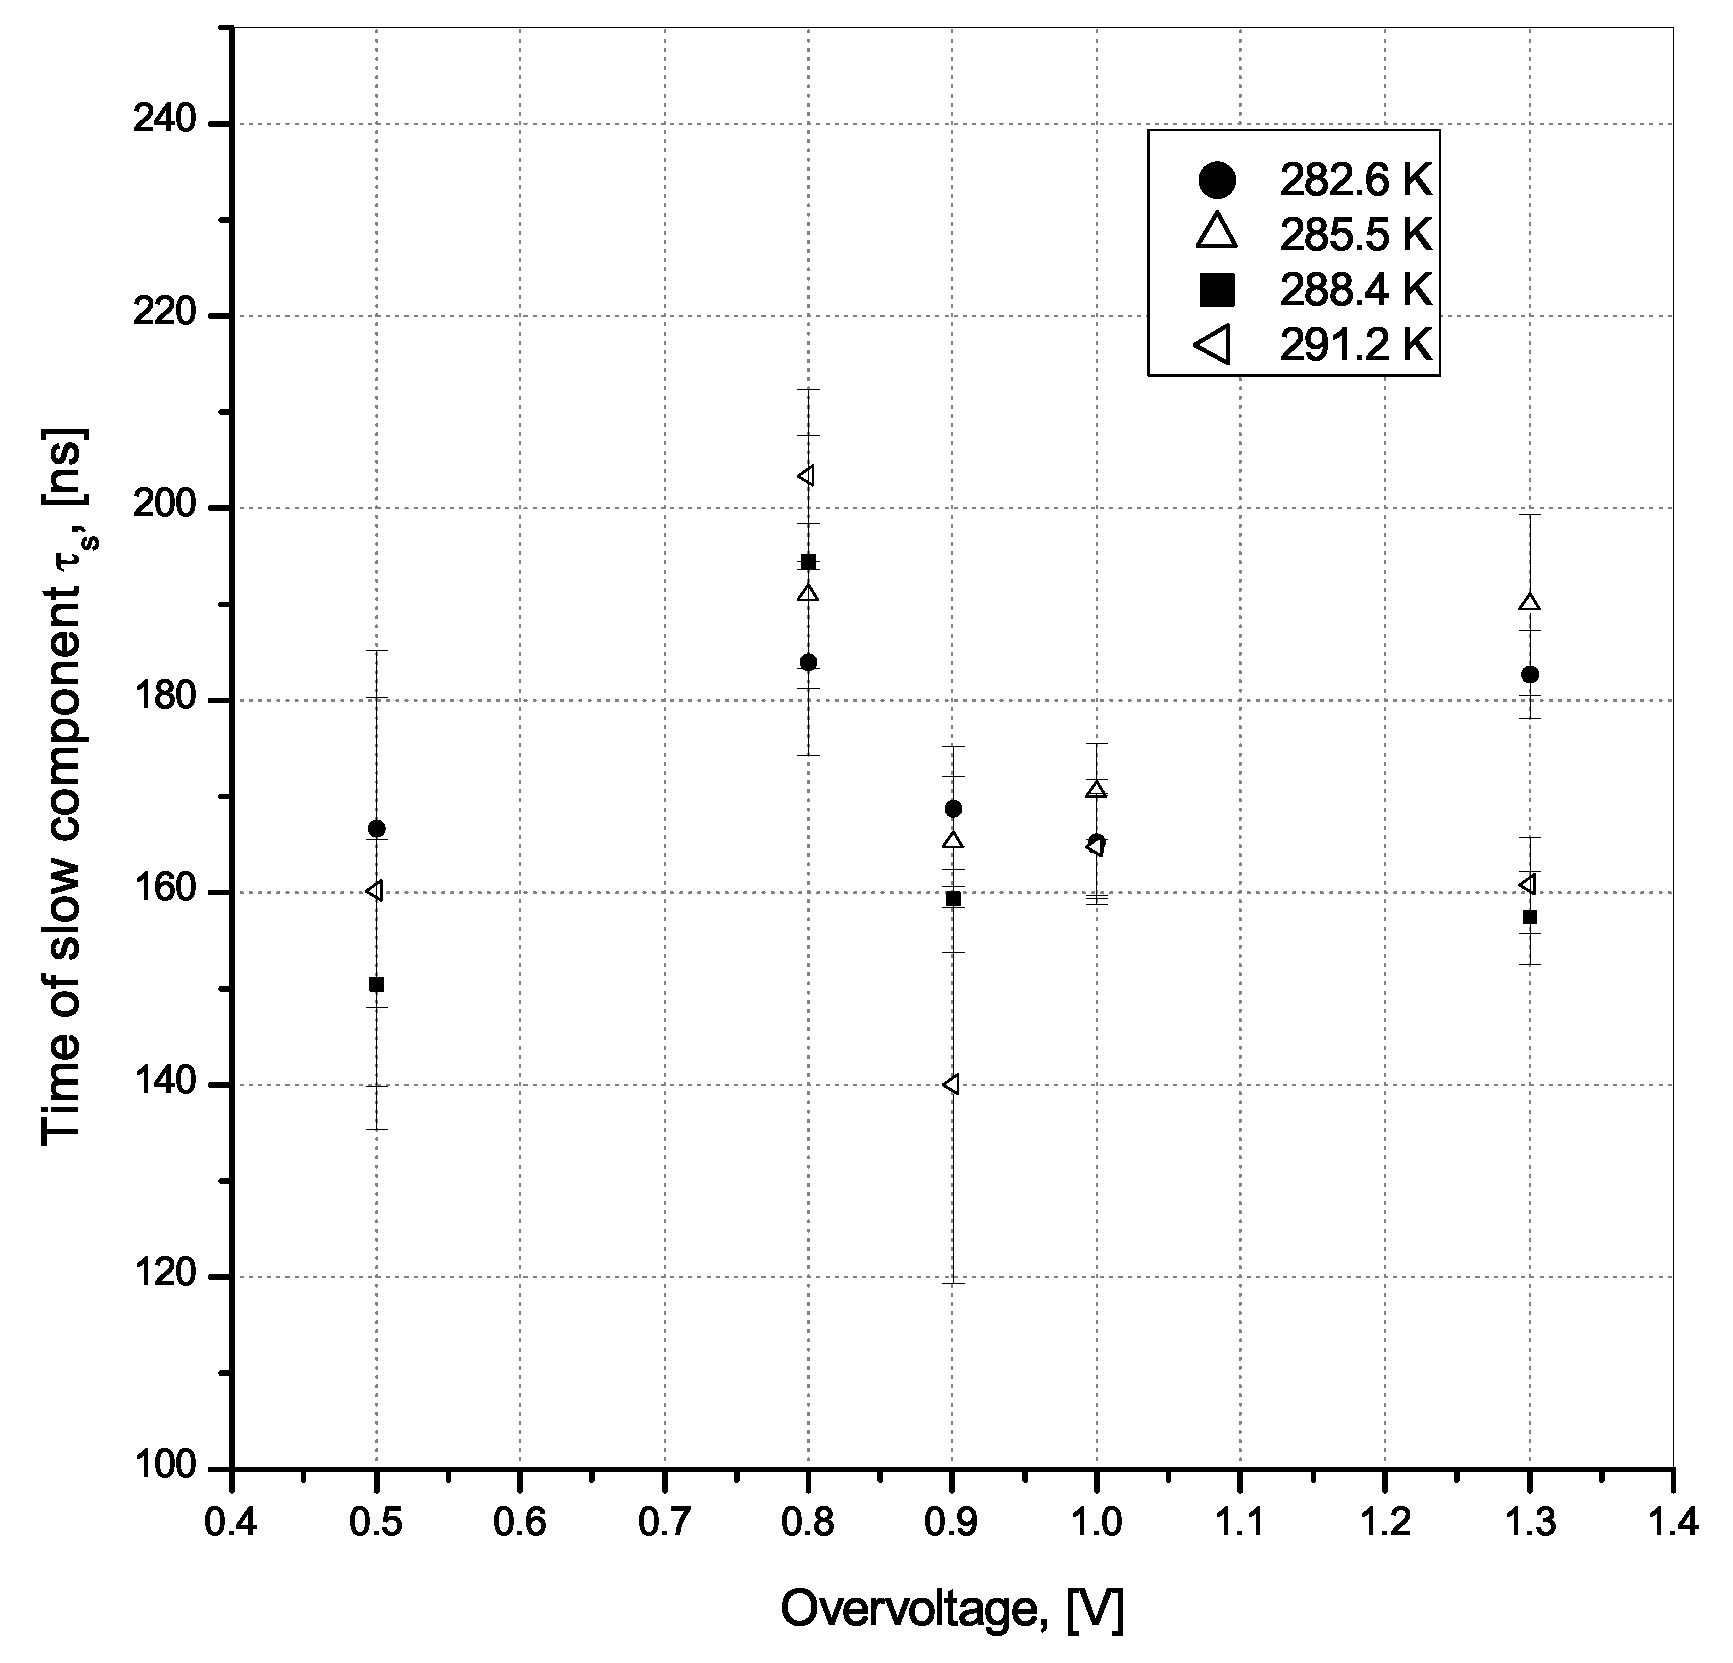
\includegraphics[width=0.47\textwidth]{Hamamatsu_S10362-11-100C_tau_s_vs_V_eng}
\\
\parbox[t]{0.47\textwidth}{\caption{The dependence of the slow time constant $\tau_{s}$ for an after-pulse on a temperature at a fixed overvoltage for
Hamamatsu S10362-11-100C.}
\label{image:Hamamatsu_S10362-11-100C_tau_s_vs_T}}
\hfill
\parbox[t]{0.47\textwidth}{\caption{The dependence of the slow time constant $\tau_{s}$ for an after-pulse on a overvoltage at a fixed temperature for
Hamamatsu S10362-11-100C.}
\label{image:Hamamatsu_S10362-11-100C_tau_s_vs_V}}
\end{figure}
%\fi

\begin{figure}[h]
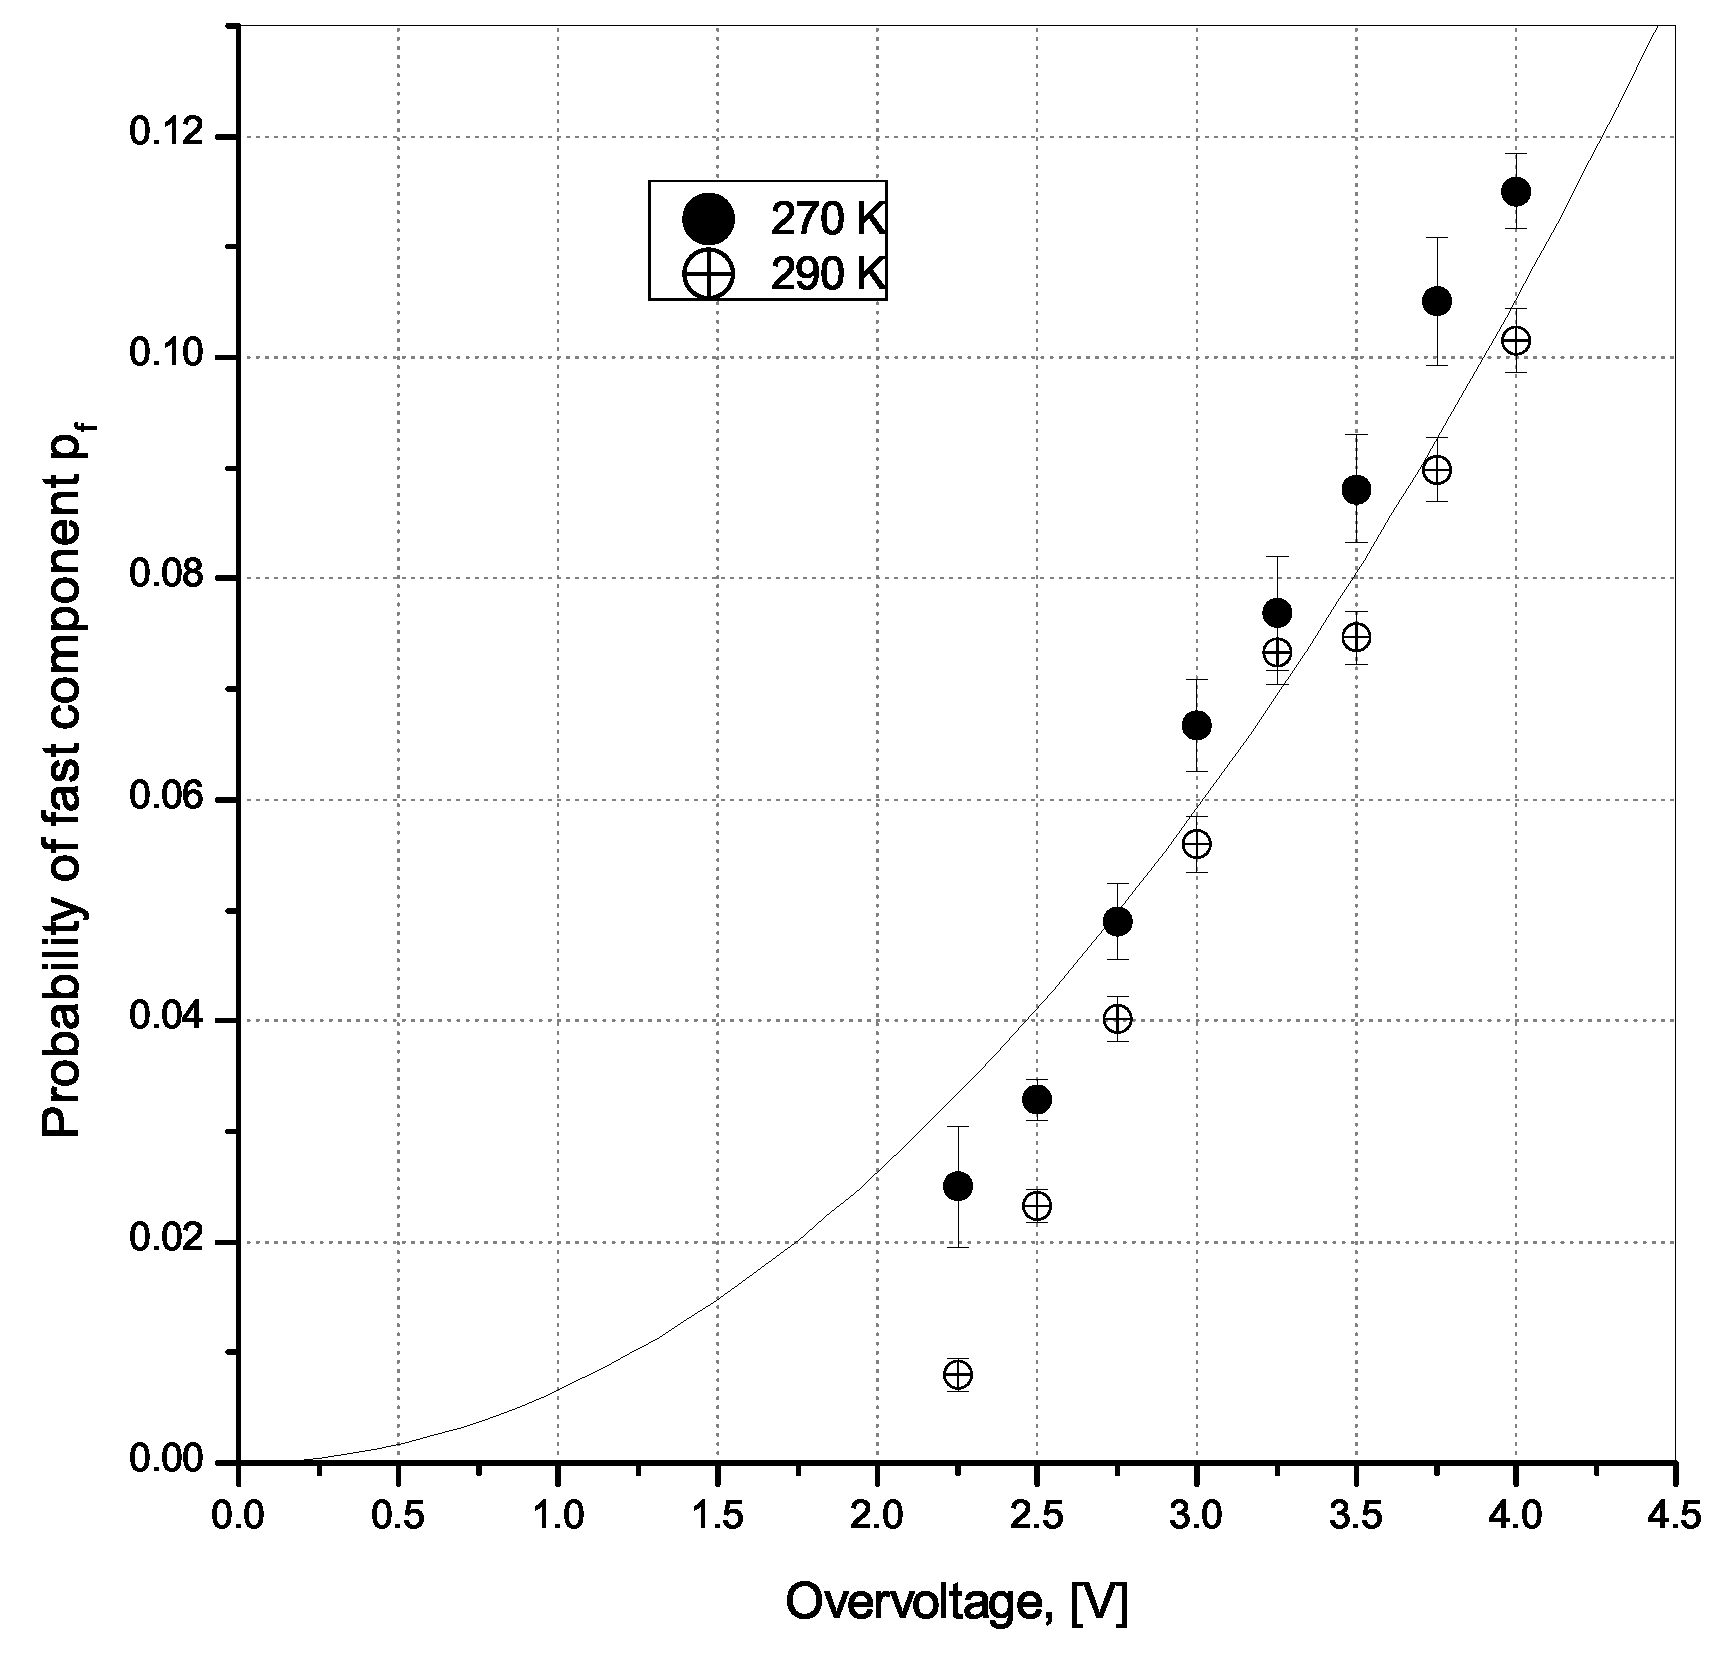
\includegraphics[width=0.47\textwidth]{Hamamatsu_S13360-3050CS_p_f_vs_V_eng}
\hfill
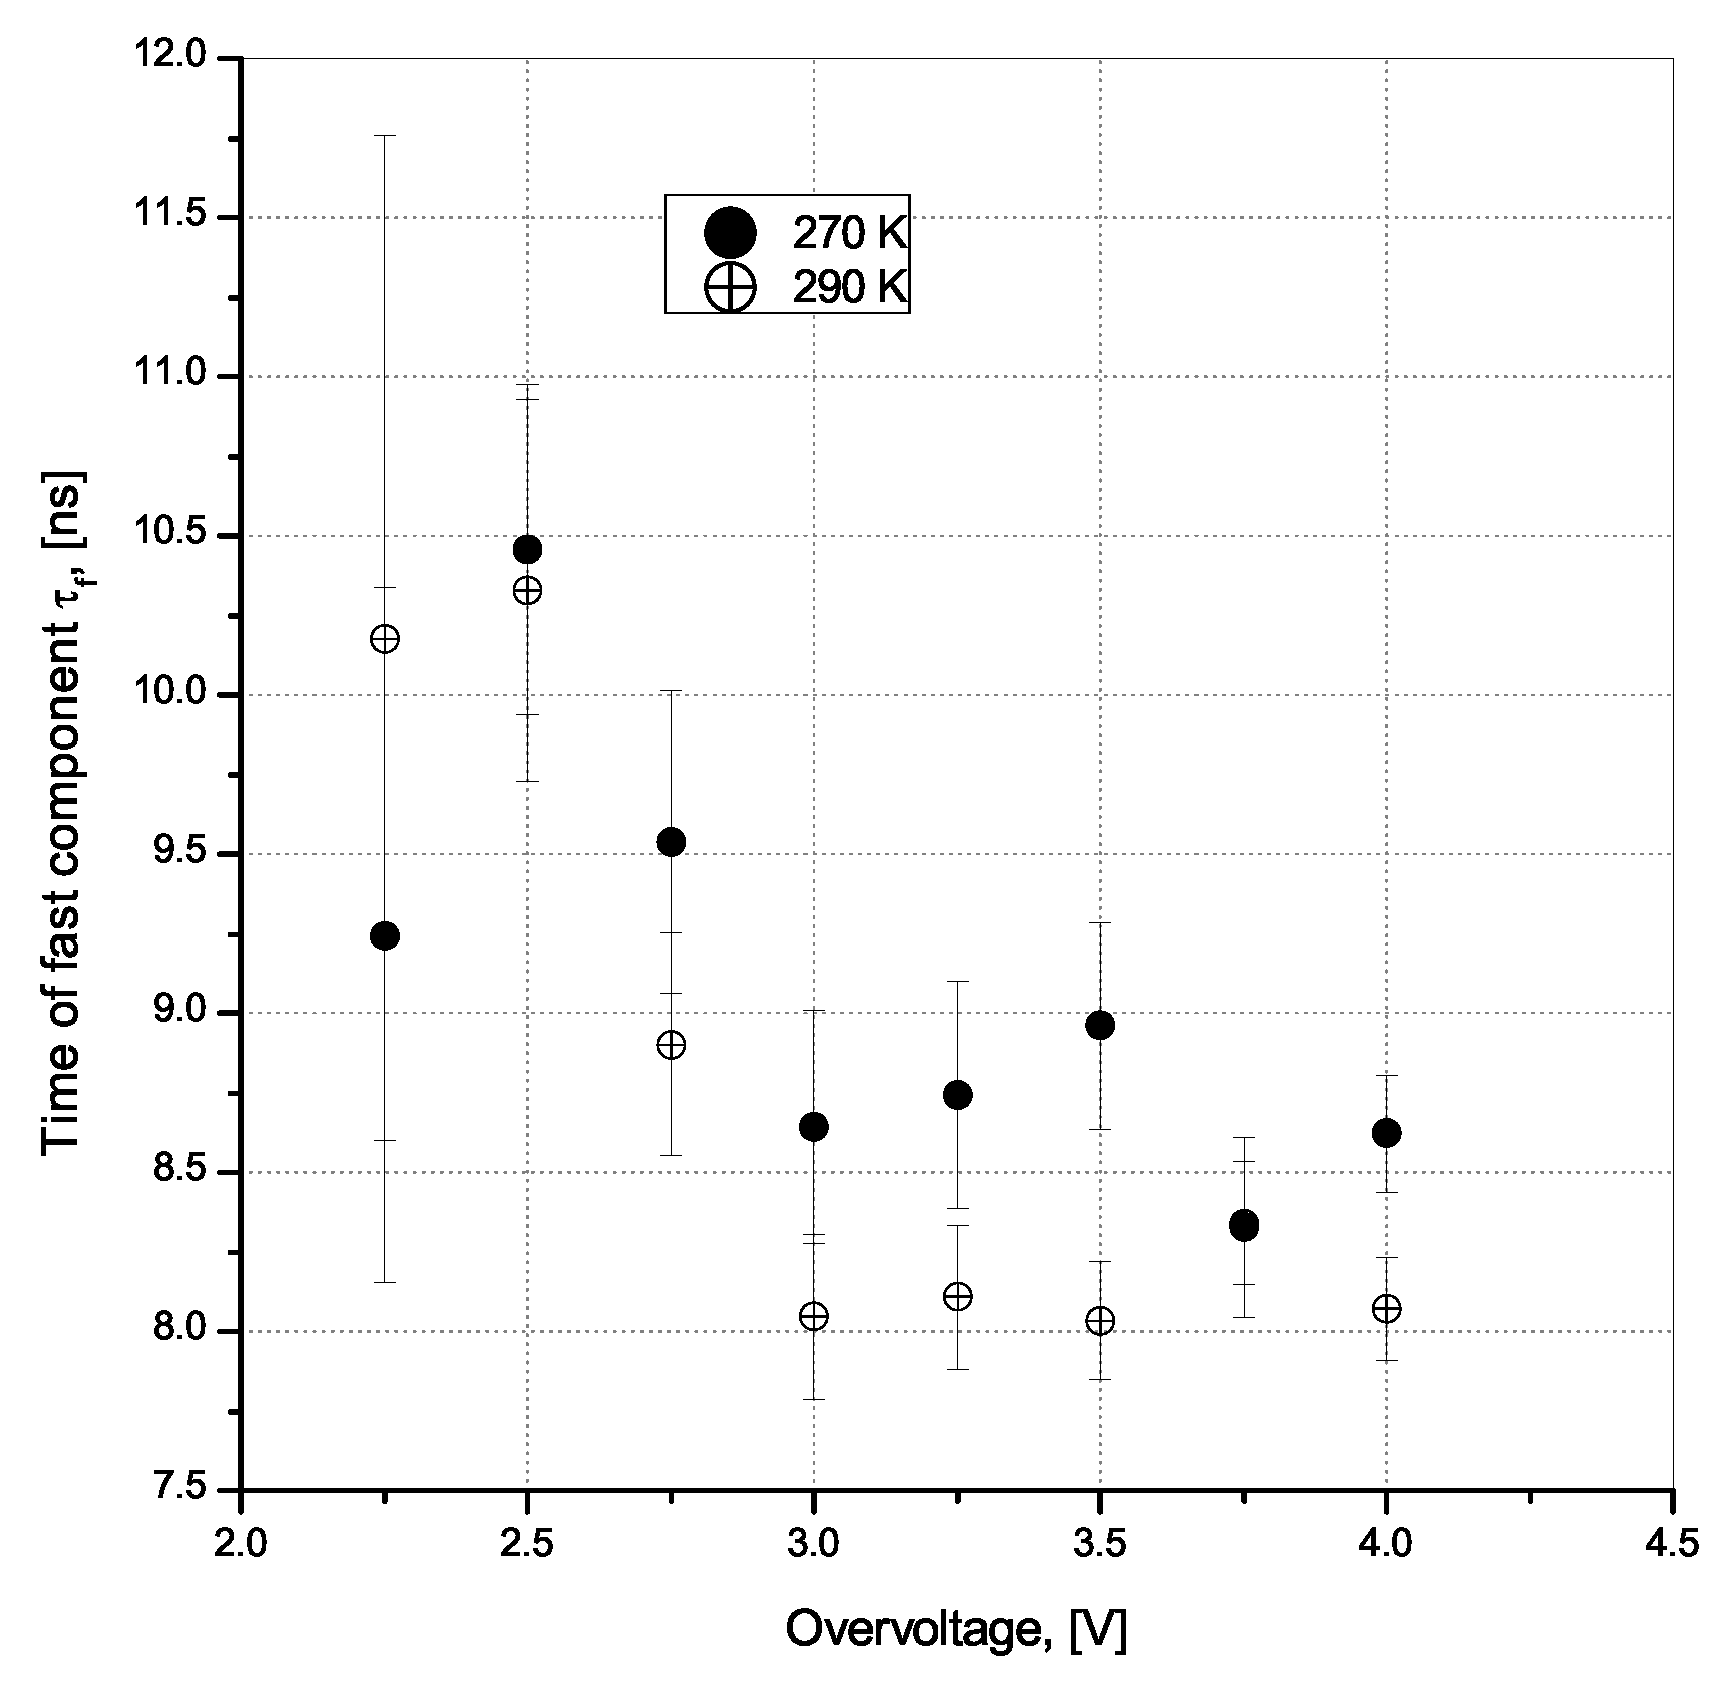
\includegraphics[width=0.47\textwidth]{Hamamatsu_S13360-3050CS_tau_f_vs_V_eng}
\\
\parbox[t]{0.47\textwidth}{\caption{The dependence of the fast component probability $p_{f}$ for an after-pulse on an overvoltage at a fixed temperature for
Hamamatsu S13360-3050CS. The data were approximated by a quadratic function.}
\label{image:Hamamatsu_S13360-3050CS_p_f_vs_V_rus}}
\hfill
\parbox[t]{0.47\textwidth}{\caption{The dependence of the fast time constant $\tau_{f}$ for an after-pulse on an overvoltage at a fixed temperature for
Hamamatsu S13360-3050CS.}
\label{image:Hamamatsu_S13360-3050CS_tau_s_vs_V}}
\end{figure}

\begin{figure}[h]
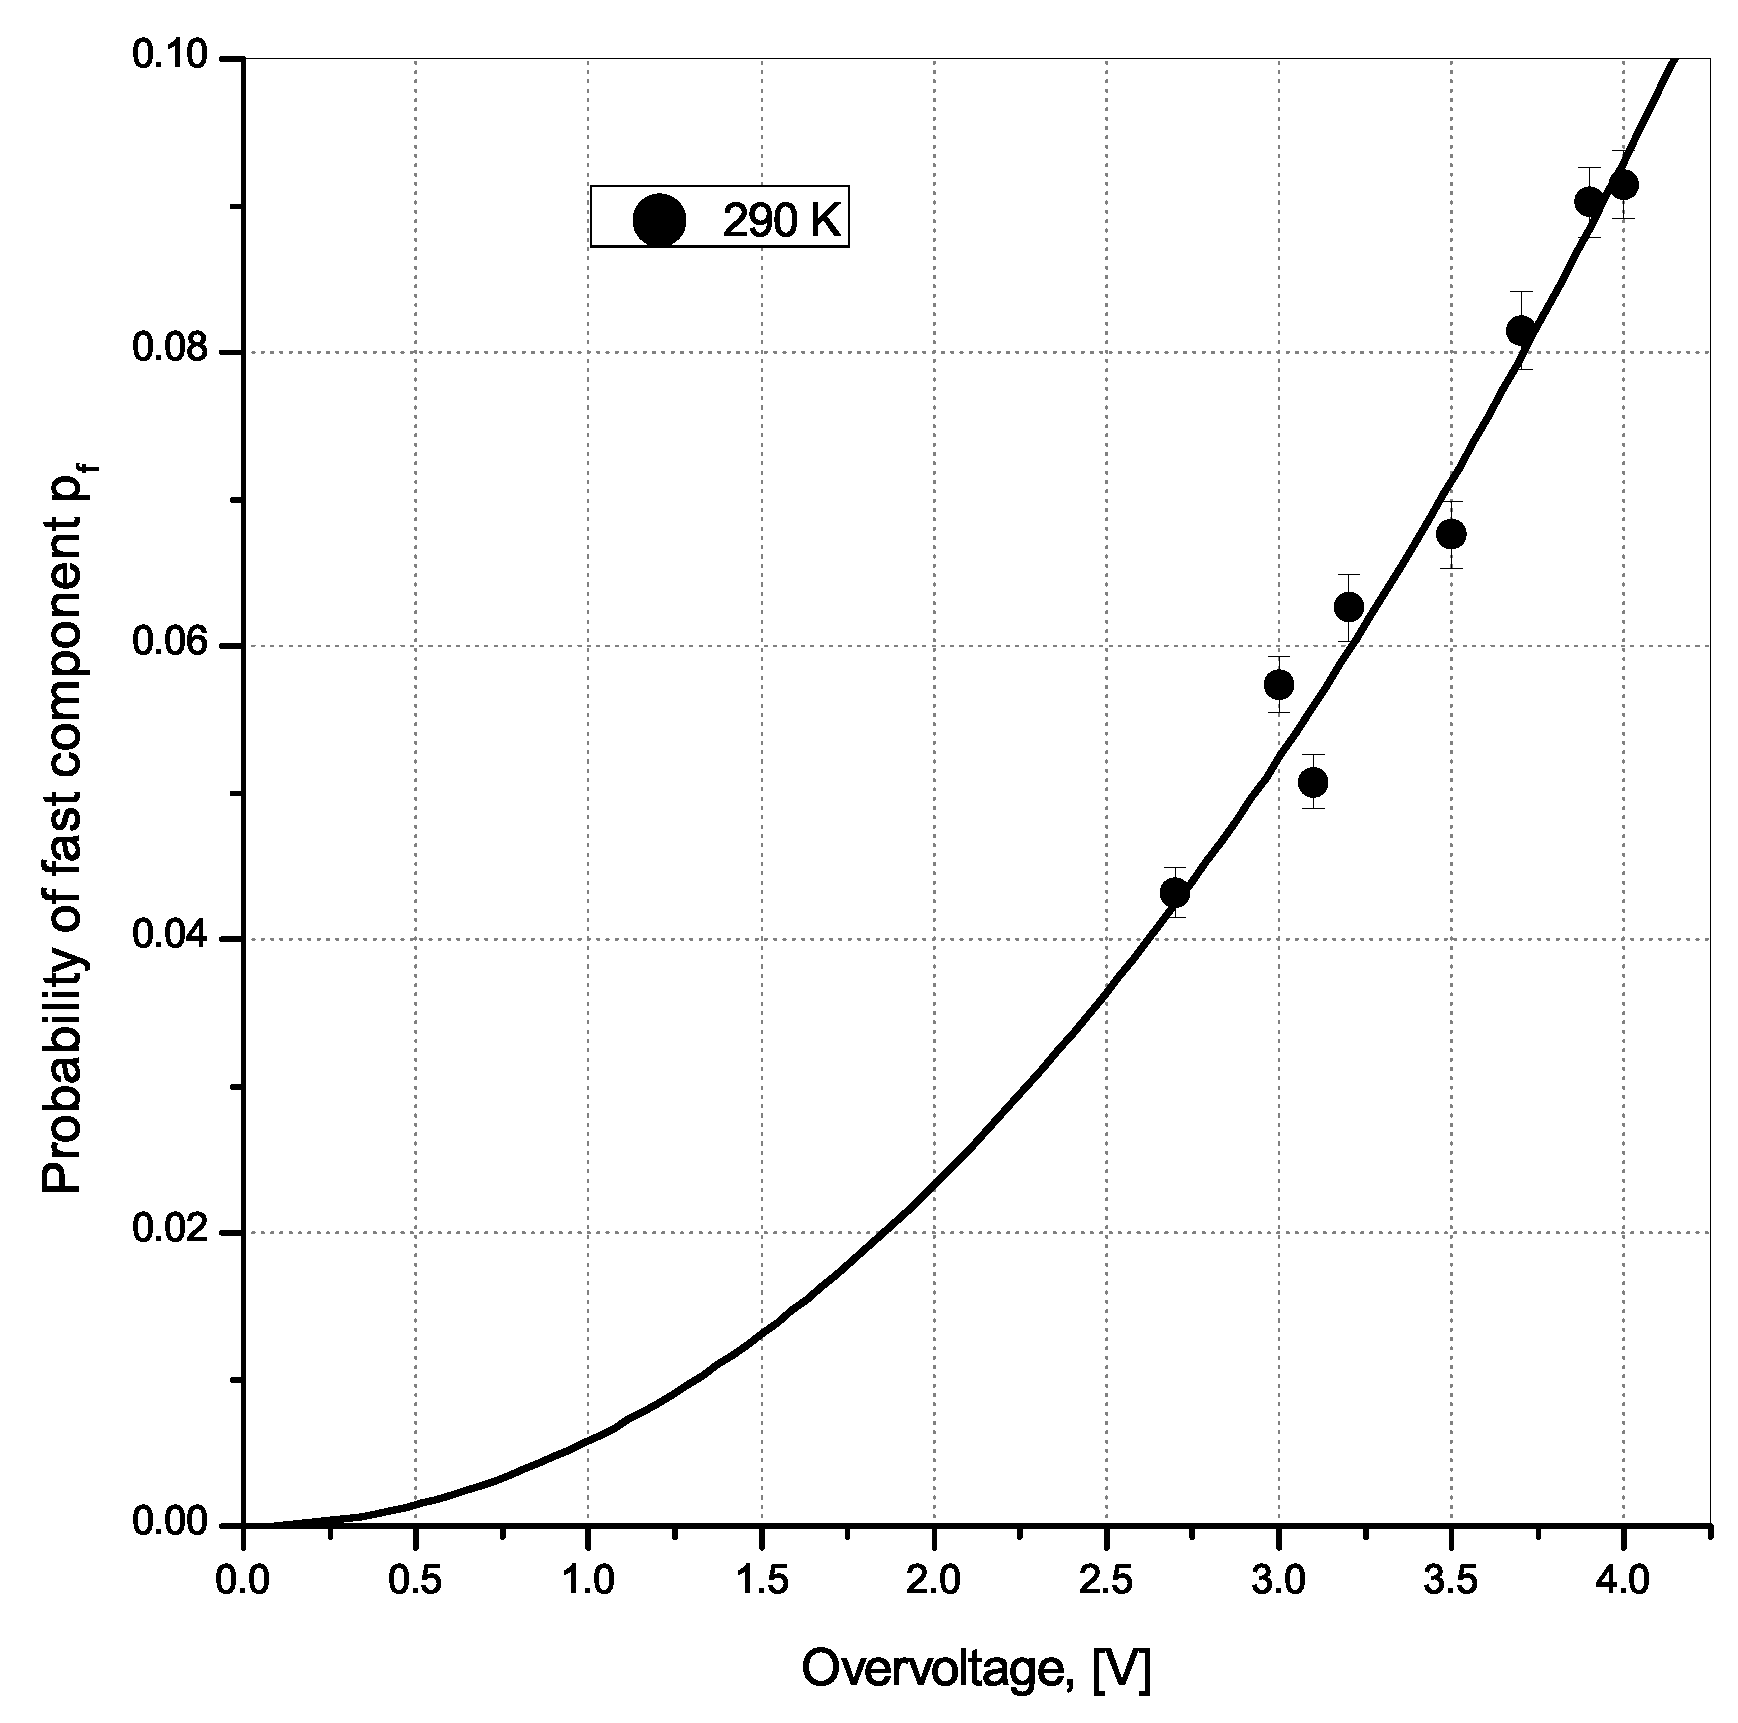
\includegraphics[width=0.47\textwidth]{KETEK_PM1125NS_SB0_p_f_vs_V_eng}
\hfill
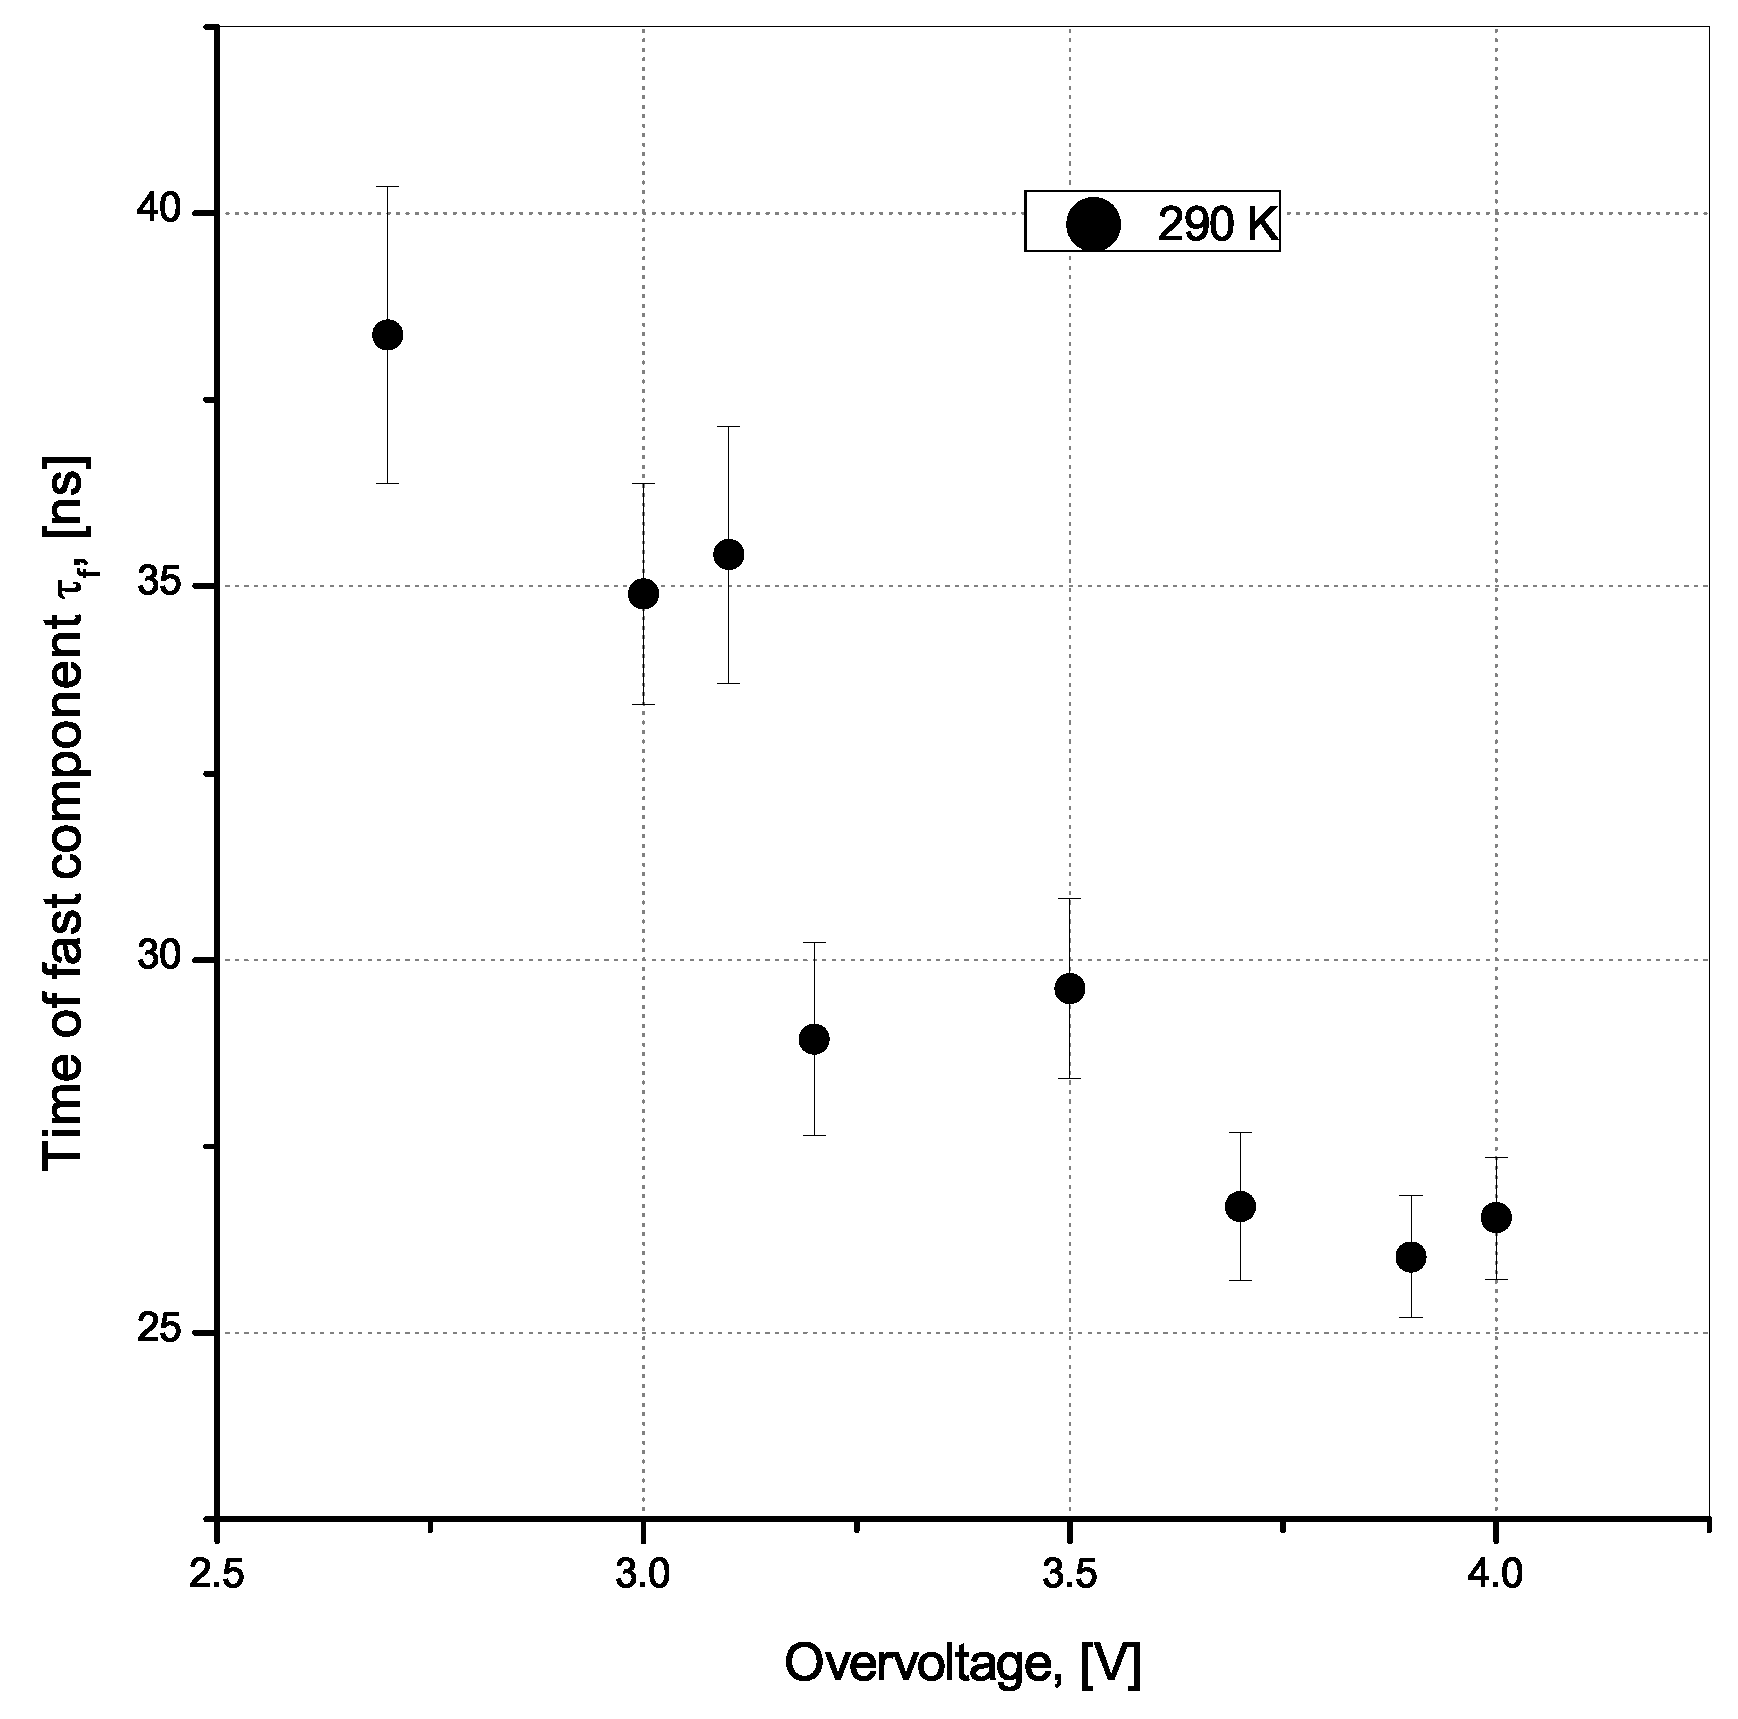
\includegraphics[width=0.47\textwidth]{KETEK_PM1125NS_SB0_tau_f_vs_V_eng}
\\
\parbox[t]{0.47\textwidth}{\caption{The dependence of the fast component probability $p_{f}$ for an after-pulse on an overvoltage at a fixed temperature for
KETEK PM1125NS-SB0. The data were approximated by a quadratic function.}
\label{image:KETEK_PM1125NS_SB0_p_f_vs_V_rus}}
\hfill
\parbox[t]{0.47\textwidth}{\caption{The dependence of the fast time constant $\tau_{f}$ for an after-pulse on an overvoltage at a fixed temperature for
KETEK PM1125NS-SB0.}
\label{image:KETEK_PM1125NS_SB0_tau_f_vs_V_rus}}
\end{figure}

After-pulse probabilities $p_{s}$ and $p_{f}$ at the current accuracy of the measurement are independent of a temperature.
At the same time, this probabilities have to have a quadratic dependence on an overvoltage:
\begin{eqnarray}\label{eq:p_f_s_vs_T_V}
p_{i}(\Delta V, T) = k_{i}^{p} \cdot \Delta V^2
\end{eqnarray}

The time constants $\tau_{s}$ and $\tau_{f}$ at a given measurement accuracy are independent on an overvoltage.

\section{Conclusions}
In the work were described the algorithms for measurement the breakdown voltage, dark noise, probabilities for cross-talk and after-pulsing and after-pulsing time constants for three SiPMs types: KETEK PM1125NS-SB0, Hamamatsu S10362-11-100C and Hamamatsu S13360-3050CS.

An offline signal processing was performed by the pulse approximation with reconstruction of amplitudes and start times to find these parameters.
Besides the algorithm used, there are three methods.
The first - the measurement of the pulse rate depending on the amplitude threshold.
The second - the integration a signal at a certain time interval and finding a number of events in the peaks.
The third -  the signal deconvolution and an approximation of the pulse interval spectrum.
The first two methods are rather simple and can be used in an online analysis
but they have a serious drawback - after-pulsing probabilities and after-pulsing time constants can't be found.
The third method, and the method used in this study require large computing power, however, allow us to find after-pulsing parameters.

At achieved measurement accuracy in the temperature range from $0$ to $20 C^{\circ}$ the cross-talk probability, after-pulsing probabilities and after-pulsing time constants are independent on a temperature.
SiPMs were checked for compliance with the four neighbors model.
All three types of SiPMs have model discrepancy less than 10\%.

The cross-talk probability for Hamamatsu S10362-11-100C at an operating overvoltage (1 V) is about 12\%, for Hamamatsu S13360-3050CS and KETEK PM1125NS-SB0 (an operating overvoltage is 4 V) is about 6\%. After-pulsing probabilities for Hamamatsu S10362-11-100C at an operating overvoltage is about 10\% (fast component) � 15\% (slow component).
For Hamamatsu S13360-3050CS and KETEK PM1125NS-SB0 because of the small statistics it was studied only the fast component, which is about 10\%.
After-pulsing time constants for Hamamatsu S10362-11-100C are about 35 ns (fast component) and 170 ns (slow component), for Hamamatsu S13360-3050CS - 9 ns, for KETEK PM1125NS-SB0 - 28 ns.
Dark noise rate for Hamamatsu S10362-11-100C at an operating overvoltage and $20  \;  ^{\circ}C$ temperature is about $300  \;  kHz / mm^2$, for Hamamatsu S13360-3050CS - $30 \; kHz / mm^2$, for KETEK PM1125NS-SB0 - $80 \; kHz / mm^2$.

Thus, on the basis of the experiments we can conclude that the best candidate for use in counting detectors among the studied SiPMs is Hamamatsu S13360-3050CS which has lower dark noise rate and the least after-pulsing time constants.


\section*{����������}
\addcontentsline{toc}{section}{����������}

� ������ ������ ������������ �������� �������������� ������ ���� ������ � ������ Ar � ������� ����������� ��������� � ��������������������� ������� � DD ���������� �����������. ������������� ������ � ������ Ar ��� 233 ��� �� ����������� ��������� ��������� ������� 5,9~$\pm$~0,8 � 7,4~$\pm$~1 e-/��� ��� ��������� �������������� ���� 0,56 � 0,62 ��/�� ��������������; ������������� ������� ������� ��������� 0,31~$\pm$~0,06 � 0,37~$\pm$~0,07 ��������������. ��� ��������� �����������, ���������� ��� ������ �������� � ������� �����, ���� ���������� ����������� ����������� �������������� ������ �� ������� � �������������� ����. � ���������, ���������������� ���������� ��������� �������������� �����������, ����� ������������� ����� �������� ����� ������� ��� ����� �������. ���������� ������� ������������ ����� ������ �������� ��� �������������� ���������� ���������� �� ������ ������ ����������� �����, ������������ ��� ������ ������ �������, � ��� ���������� ��������� ������������� ������� � ������ Ar. 
\begin{thebibliography}{99}

\bibitem{Detectors for Dark Matter search (Review)}
Akimov D. Detectors for Dark Matter search (Review) // Nucl. Instrum. Meth. A. 2009. Vol. 598. P. 275. 

\bibitem{Advances in Cryogenic Avalanche Detectors}
Buzulutskov A. Advances in Cryogenic Avalanche Detectors // J. of Instrumentation. 2012. Vol. 7. C02025. 

\bibitem{Liquid Noble Gas Detectors for Low Energy Particle Physics}
Chepel V., Araujo H. Liquid Noble Gas Detectors for Low Energy Particle Physics // J. of Instrumentation. 2013. Vol. 8. R04001. 

\bibitem{New Results from DAMA/LIBRA}
Bernabei R. et al. New Results from DAMA/LIBRA // Eur. Phys. J. C. 2010. Vol. 67. P. 39. 

\bibitem{CoGeNT: A Search for Low-Mass Dark Matter using p-type Point Contact Germanium Detectors}
Aalseth C. E. et al. CoGeNT: A Search for Low-Mass Dark Matter using p-type Point Contact Germanium Detectors // Eprint arXiv:1208.5737. 2012.

\bibitem{Results from 730 kg Days of the CRESST-II Dark Matter search}
Angloher G. et al. Results from 730 kg Days of the CRESST-II Dark Matter search // Eur. Phys. J. C. 2012. Vol. 72. P. 1971. 

\bibitem{Dark Matter Search Results Using the Silicon Detectors of CDMS II}
Agnese R. et al. Dark Matter Search Results Using the Silicon Detectors of CDMS II // Eprint arXiv:1304.4279. 2013. 

\bibitem{Search for Light Dark Matter in XENON10 Data}
Angle J. et al. Search for Light Dark Matter in XENON10 Data // Phys. Rev. Lett. 2011. Vol. 107. 051301. 

\bibitem{Dark Matter Results from 225 Live Days of XENON100 Data}
Aprile E. at al. Dark Matter Results from 225 Live Days of XENON100 Data // Phys. Rev. Lett. 2012. Vol. 109. 181301.

\bibitem{WIMP-Nucleon CrossSection Results from the Second Science Run of ZEPLIN-III}
Akimov D. et al. WIMP-Nucleon CrossSection Results from the Second Science Run of ZEPLIN-III // Phys. Lett. B. 2012. Vol. 709. P. 14.  

\bibitem{Two-Phase Emission Detector for Measuring Coherent Neutrino-Nucleus Scattering}
Hagmann C., Bernstein A. Two-Phase Emission Detector for Measuring Coherent Neutrino-Nucleus Scattering // IEEE Trans. Nucl. Sci. 2004. Vol. 51. P. 2151. 

\bibitem{Detection of Reactor Antineutrino Coherent Scattering off Nuclei with a Two-Phase Noble Gas Detector}
Akimov D. et al. Detection of Reactor Antineutrino Coherent Scattering off Nuclei with a Two-Phase Noble Gas Detector // J. of Instrumentation. 2009. Vol. 4. P06010. 

\bibitem{Comments on "First Dark Matter Results from the XENON100 Experiment"}
Collar J. I., McKinsey D. N. Comments on �First Dark Matter Results from the XENON100 Experiment� // Eprint arXiv:1005.0838. 2010.

\bibitem{A Coherent Understanding of Low-Energy Nuclear Recoils in Liquid Xenon}
Sorensen P. A Coherent Understanding of Low-Energy Nuclear Recoils in Liquid Xenon // J. Cosmol. Astropart. Phys. 2010. Vol. 9. 033. 

\bibitem{Neutrino Detection with CLEAN}
McKinsey D. N., Coakley K. J. Neutrino Detection with CLEAN // Astropart. Phys. 2005. Vol. 22. P. 355. 

\bibitem{A Concept for a Dark Matter Detector Using Liquid Helium-4}
Guo W., McKinsey D. N. A Concept for a Dark Matter Detector Using Liquid Helium-4 // Eprint arXiv:1302.0534. 2013. 

\bibitem{A Survey of Energy Loss Calculations for Heavy Ions between 1 and 100 kev}
Mangiarotti A. et al. A Survey of Energy Loss Calculations for Heavy Ions between 1 and 100 kev // Nucl. Instrum. Meth. A. 2007. Vol. 580. P. 114. 

\bibitem{A Model of Nuclear Recoil Scintillation Efficiency in Noble Liquids}
Mei D.-M. et al. A Model of Nuclear Recoil Scintillation Efficiency in Noble Liquids // Astropart. Phys. 2008. Vol. 30. P. 12. 

\bibitem{Ionization Efficiency Study for Low Energy Nuclear Recoils in Germanium}
Barker D. et al. Ionization Efficiency Study for Low Energy Nuclear Recoils in Germanium // Eprint arXiv: 1304.6773. 2013. 

\bibitem{Quenching and Channeling of Nuclear Recoils in NaI[Tl]: Implications for Dark Matter Searches}
Collar J.I. Quenching and Channeling of Nuclear Recoils in NaI[Tl]: Implications for Dark Matter Searches // Eprint: arXiv:1302. 0796. 2013.

\bibitem{Scintillation Efficiency and Ionization Yield of Liquid Xenon for Monoenergetic Nuclear Recoils down to 4 keV}
Manzur A. et al. Scintillation Efficiency and Ionization Yield of Liquid Xenon for Monoenergetic Nuclear Recoils down to 4 keV // Phys. Rev. C. 2010. Vol. 81. 025808. 

\bibitem{Nuclear Recoil Scintillation and Ionisation Yields in Liquid Xenon from ZEPLIN-III Data}
Horn M. et al. Nuclear Recoil Scintillation and Ionisation Yields in Liquid Xenon from ZEPLIN-III Data // Phys. Lett. B. 2011. Vol. 705. P. 471. 

\bibitem{New Measurement of the Scintillation Efficiency of Low-Energy Nuclear Recoils in Liquid Xenon}
Plante G. et al. New Measurement of the Scintillation Efficiency of Low-Energy Nuclear Recoils in Liquid Xenon // Phys. Rev. C. 2011. Vol. 84. 045805. 

\bibitem{Measurement of Scintillation Efficiency for Nuclear Recoils in Liquid Argon}
Gastler D. et al. Measurement of Scintillation Efficiency for Nuclear Recoils in Liquid Argon // Phys. Rev. C. 2012. Vol. 85. 065811. 

\bibitem{Study of Nuclear Recoils in Liquid Argon with Monoenergetic Neutrons}
Regenfus C. et al. Study of Nuclear Recoils in Liquid Argon with Monoenergetic Neutrons // J. Phys.: Conf. Ser. 2012. Vol. 375. 012019. 

\bibitem{Scintillation Yield and Time Dependence from Electronic and Nuclear Recoils in Liquid Neon}
Lippincott W. H. et al. Scintillation Yield and Time Dependence from Electronic and Nuclear Recoils in Liquid Neon // Phys. Rev. C. 2012. Vol. 86. 015807. 


\end{thebibliography}


\chapter*{���������� �. ������ �������������� � ����������� � ���������� ������}
\addcontentsline{toc}{chapter}{���������� �. ������ �������������� � ����������� � ���������� ������}

�������������� ������:
\begin{enumerate}
  \item Babichev E.A. et al. SiPM based photon counting detector for scanning digital radiography //
  \href{https://doi.org/10.1088/1748-0221/10/03/C03002}{J. of Instrumentation. 2015. Vol. 10. C03002.}

  \item Babichev E.A. et al. Photon counting detector for the personal radiography inspection system �SIBSCAN� //
  \href{https://doi.org/10.1016/j.nima.2016.06.051}{Nucl. Instrum. Meth. A. 2017. Vol. 845. P. 499.}

  \item Kuper K.E. et al. On reachable energy resolution of SiPM based scintillation counters for X-ray detection //
  \href{https://doi.org/10.1088/1748-0221/12/01/P01001}{J. of Instrumentation. 2017. Vol. 12. P01001.}
  
  \item Oleynikov V. and Porosev V. After-pulsing and cross-talk comparison for PM1125NS-SB0 (KETEK), S10362-11-100C (HAMAMATSU) and S13360-3050CS (HAMAMATSU) //
  \href{https://doi.org/10.1088/1748-0221/12/06/C06046}{J. of Instrumentation. 2017. Vol. 12. C06046.}

  \item Bondar A. et al. Measurement of the ionization yield of nuclear recoils in liquid argon using a two-phase detector with electroluminescence gap // \\
  \href{https://doi.org/10.1088/1748-0221/12/05/C05010}{J. of Instrumentation. 2017. Vol. 12. C05010.}

  \item Bondar A. et al. Further studies of proportional electroluminescence in two-phase argon //
  \href{https://doi.org/10.1088/1748-0221/12/05/C05016}{J. of Instrumentation. 2017. Vol. 12. C05016.}
  
  \item Aalseth C. E. et al. Cryogenic Characterization of FBK RGB-HD SiPMs //
  \href{https://doi.org/10.1088/1748-0221/12/09/P09030}{J. of Instrumentation. 2017. Vol. 12. P09030.}
  
  \item ������� �. �. � ��. ������������ ���������������� �������������������� � ���������� ������ //
  doi 10.25205/2541-9447-2017-12-3-5-15 ��������� ���������� ������. 2017. ��� 12. �3.
  
  \item ������� �. �. � ��. ��������� ������������� ������� ���� ������ � ������ ������ � ������� ����������� ��������� � ���������� ����������� //
  doi 10.25205/2541-9447-2017-12-3-16-23 ��������� ���������� ������. 2017. ��� 12. �3.  

  
\end{enumerate}

��������� � ����������:
\begin{enumerate}
  \item ��������� ������� ��������� ������������� ������� ���� ������ � ������ ������ ������� ��������� ��������� � ���������� ��������� //
  ������ ���� (������ ������������ ������ � �������� ����). ����� ������������ � 4-� ������� � 2018 ����.
\end{enumerate}

\section*{���������� �. ������ ����������� �� ������� ������������} 
\addcontentsline{toc}{section}{���������� �. ������ ����������� �� ������� ������������} \begin{enumerate}
  \item ������������� ������� ������������ �����������, �����������, 2012. ������ 3-� �������.
  \item ������� ������� ������, ��� �� ���, �����������, 2014. ������ 3-� �������.
  \item ������������� ������� ������������ �����������, �����������, 2014. ������ 3-� �������.
  \item The 14th Vienna Conference on Instrumentation (VCI2016), ����, 15-19 ������� 2016. ��������� ������.  
  \item ������� ������� ������, ��� �� ���, �����������, 2016.
  \item Instrumentation for Colliding Beam Physics (INSTR17) Conference, �����������, 2017. ������ ������.
  \item Instrumentation for Colliding Beam Physics (INSTR17) Conference, �����������, 2017. ��������� ������.
  \item ������� ������� ������, ��� �� ���, �����������, 2017. ������ 2-� �������.
  \item International Session-Conference of the Section of Nuclear Physics of the Physical Sciences Department of the Russian Academy of Sciences, �������, 2017. ������ ������.
\end{enumerate}

\end{document}
